\chapter{Experimentos e Resultados}
\label{cap:resultados}

\section{Reprodutibilidade}

Esta seção detalha os aspectos técnicos necessários para a reprodução dos experimentos realizados neste trabalho. A implementação segue uma formulação baseada em Processo de Decisão de Markov Parcialmente Observável Descentralizado (Dec-POMDP), com detalhamento do ambiente de simulação, configurações, estados, ações, função de recompensa e toda a estrutura de Curriculum Learning implementada.

\subsection{Formulação Dec-POMDP}

O problema de controle multiagente em futebol de robôs é formulado como um Dec-POMDP, representado pela tupla:

$$G = \langle D, A, S, Z, P, R \rangle.$$

Onde:
\begin{itemize}
    \item $D$: Conjunto de agentes robóticos que participam do jogo;
    \item $A$: Espaço de ações disponíveis para cada agente;
    \item $S$: Espaço de estados do ambiente (não completamente observável pelos agentes);
    \item $Z$: Espaço de observações parciais que cada agente recebe;
    \item $P$: Função de transição que determina a dinâmica do ambiente;
    \item $R$: Função de recompensa que guia o aprendizado dos agentes.
\end{itemize}

A formulação Dec-POMDP é particularmente adequada para este domínio, pois os agentes precisam tomar decisões baseadas em observações locais parciais, enquanto colaboram para alcançar objetivos comuns, como marcar gols e evitar que o adversário marque.

\subsection{Conjunto de Agentes $D$}

O conjunto de agentes varia conforme o estágio do curriculum learning e o tipo de experimento. A configuração padrão para o jogo completo é:

$$D_{azul} = \{d_1, d_2, d_3\}$$ para o time azul e $$D_{amarelo} = \{d_4, d_5, d_6\}$$ para o time amarelo.

O número de agentes é dinamicamente ajustado durante as diferentes fases do curriculum learning:

\begin{itemize}
    \item \textbf{Curriculum Task 0 (Fundamentos Básicos)}: $D_{azul} = \{d_1\}$ e $D_{amarelo} = \{\emptyset\}$ (nenhum agente adversário);
    \item \textbf{Curriculum Task 1 (Interação com Oponentes Estáticos)}: $D_{azul} = \{d_1, d_2, d_3\}$ e $D_{amarelo} = \{d_4\}$ (apenas um agente adversário estático);
    \item \textbf{Self-play}: $D_{azul} = \{d_1, d_2, d_3\}$ e $D_{amarelo} = \{d_4, d_5, d_6\}$ (configuração completa).
\end{itemize}

Todos os agentes de um mesmo time compartilham os mesmos parâmetros de política (policy sharing), o que facilita o aprendizado coletivo e reduz a dimensionalidade do problema. Essa abordagem de compartilhamento de política permite que comportamentos emergentes de coordenação surjam naturalmente durante o treinamento.

\subsection{Espaço de Ações $A$}

Cada agente possui um espaço de ação contínuo com 4 dimensões:

$$a_d = (v_x, v_y, \omega_{\theta}, k) \in [-1.0, 1.0]^4.$$

Onde:
\begin{itemize}
    \item $v_x$: Velocidade normalizada no eixo x (movimento lateral);
    \item $v_y$: Velocidade normalizada no eixo y (movimento frontal);
    \item $\omega_{\theta}$: Velocidade angular normalizada (rotação);
    \item $k$: Ação de chute (contínua, onde valores > 0 executam o chute).
\end{itemize}

Estas ações de alto nível são convertidas para comandos de baixo nível das quatro rodas do robô usando a cinemática do robô omnidirecional. A conversão segue o seguinte processo:

\subsubsection{Transformação de coordenadas}

Primeiro, as velocidades no referencial global são transformadas para o referencial local do robô:
$$v_x', v_y' = v_x \cdot \cos(\theta) + v_y \cdot \sin(\theta), -v_x \cdot \sin(\theta) + v_y \cdot \cos(\theta).$$

Onde $\theta$ é a orientação atual do robô.

\subsubsection{Cálculo das velocidades angulares das rodas}

Em seguida, as velocidades locais e a velocidade angular são convertidas para comandos de velocidade das quatro rodas omnidirecionais:
$$\omega_{roda0} = \frac{v_y'}{r} - \frac{L \cdot \omega_{\theta}}{r}.$$
$$\omega_{roda1} = \frac{v_x'}{r} + \frac{L \cdot \omega_{\theta}}{r}.$$
$$\omega_{roda2} = -\frac{v_y'}{r} - \frac{L \cdot \omega_{\theta}}{r}.$$
$$\omega_{roda3} = -\frac{v_x'}{r} + \frac{L \cdot \omega_{\theta}}{r}.$$

Onde $r$ é o raio das rodas e $L$ é a distância do centro do robô até as rodas.

\subsubsection{Desnormalização e limitação}

Os valores normalizados são desnormalizados para as velocidades físicas reais:
\begin{itemize}
    \item Velocidades lineares são multiplicadas por 1.5 m/s
    \item Velocidade angular é multiplicada por 10 rad/s
\end{itemize}

Os valores resultantes são limitados às velocidades máximas permitidas pelos atuadores do robô. Esta abordagem permite que os agentes aprendam comportamentos complexos emergentes, como driblar, passar e defender, a partir deste conjunto de ações de baixo nível.

\subsection{Espaço de Estados $S$}

O estado completo $S$ do ambiente representa todas as informações físicas do sistema simulado, incluindo:

\begin{itemize}
    \item Posição $(x, y)$ e orientação $\theta$ de todos os robôs;
    \item Velocidades lineares $(v_x, v_y)$ e angulares $\omega$ de cada robô;
    \item Posição $(x, y)$ e velocidade $(v_x, v_y)$ da bola;
    \item Estado dos atuadores (velocidades das rodas);
    \item Forças e interações físicas entre todos os objetos do ambiente;
    \item Informações sobre limites do campo, área de gol e outras regiões relevantes.
\end{itemize}

Este estado completo é gerenciado pelo simulador RL-SSL-EL, que implementa a física do ambiente. No entanto, os agentes não têm acesso direto a todas essas informações, apenas a um conjunto de observações parciais derivadas do estado completo, muitas vezes com ruído adicionado para simular imperfeições sensoriais.

A formulação como Dec-POMDP é particularmente adequada neste contexto, pois reconhece que cada agente tem uma visão parcial e potencialmente ruidosa do ambiente, precisando tomar decisões com informação incompleta, semelhante ao problema enfrentado por robôs reais em um jogo físico.

\subsection{Espaço de Observações $Z$}

Cada agente $d$ recebe uma observação parcial $z_d \in Z$ do estado do ambiente. Esta observação é um vetor de 77 valores que inclui informações relevantes para a tomada de decisão do agente. Para capturar aspectos temporais e dinâmicos do jogo, estas observações são empilhadas com as 7 observações anteriores, resultando em um vetor final de entrada com 616 valores (8 × 77).

O vetor de observação é composto pelas seguintes categorias de informação:

\subsubsection{Posições Cartesianas}
\begin{itemize}
    \item Posição $(x, y)$ normalizada do próprio robô relativa ao centro do campo;
    \item Posições $(x, y)$ normalizadas dos companheiros de time relativas ao centro do campo;
    \item Posições $(x, y)$ normalizadas dos adversários relativas ao centro do campo;
    \item Posição $(x, y)$ normalizada da bola relativa ao centro do campo.
\end{itemize}

\subsubsection{Orientações Angulares}
\begin{itemize}
    \item Seno e cosseno da orientação do próprio robô para representação contínua sem descontinuidades;
    \item Arcotangente da orientação do próprio robô como informação complementar;
    \item Seno, cosseno e arcotangente dos ângulos formados entre o robô e seus aliados;
    \item Seno, cosseno e arcotangente dos ângulos formados entre o robô e os adversários;
    \item Seno, cosseno e arcotangente dos ângulos formados entre a bola e o centro de cada gol.
\end{itemize}

\subsubsection{Distâncias Euclidianas}
\begin{itemize}
    \item Entre o robô e cada companheiro de time;
    \item Entre o robô e cada adversário;
    \item Entre o robô e a bola;
    \item Entre a bola e ambos os gols (aliado e adversário).
\end{itemize}

\subsubsection{Informações Temporais e Contextuais}
\begin{itemize}
    \item Ações anteriores de todos os companheiros de time no tempo $t-1$;
    \item Tempo restante no episódio (normalizado para o intervalo $[0,1]$).
\end{itemize}

Todas as observações são normalizadas para o intervalo $[-1.0, 1.0]$ para facilitar o treinamento da rede neural. A normalização é realizada dividindo os valores brutos por constantes específicas para cada tipo de dado:
\begin{itemize}
    \item Posições: divididas pelo tamanho máximo do campo;
    \item Distâncias: divididas pela diagonal do campo;
    \item Velocidades: divididas pelas velocidades máximas permitidas.
\end{itemize}

O empilhamento temporal de 8 frames a 10Hz (correspondendo a 0.8 segundos de jogo) permite que o agente infira informações sobre velocidades e trajetórias, mesmo sem acesso direto a estes dados. Esta representação do estado foi cuidadosamente projetada para fornecer ao agente informações suficientes para tomar decisões tático-estratégicas eficazes.

\subsection{Função de Transição $P$}

A função de transição $P(s' | s, a)$ representa a dinâmica do ambiente, determinando como o estado $s$ evolui para o próximo estado $s'$ após a execução da ação conjunta $a$ por todos os agentes. No contexto deste trabalho, a dinâmica é implementada pelo ambiente de simulação \textit{RL-SSL-EL}, que oferece simulação física do futebol de robôs, incluindo movimentação dos robôs, dinâmica da bola, e interações entre os agentes no campo.

\subsubsection{Dinâmica Física Simulada}

A simulação inclui todos os aspectos físicos relevantes:

\begin{itemize}
    \item \textbf{Robôs}: Modelados como corpos rígidos com quatro rodas independentes, massa e momento de inércia realistas;
    \item \textbf{Bola}: Modelada como uma esfera com propriedades físicas apropriadas para simulação de deslizamento, rolamento e colisões;
    \item \textbf{Colisões}: Detecção de colisões entre robôs, bola e limites do campo;
    \item \textbf{Atrito}: Implementação de atrito entre diferentes superfícies, tanto estático quanto dinâmico;
    \item \textbf{Mecanismo de chute}: Simulação da força aplicada à bola quando a ação de chute é ativada.
\end{itemize}

\subsubsection{Regras do Jogo}

Além da física pura, a função de transição também implementa as regras específicas do jogo de futebol de robôs:

\begin{itemize}
    \item \textbf{Resets após gol}: Quando um gol é marcado, todos os robôs e a bola são reposicionados para as suas posições iniciais;
    \item \textbf{Resets laterais}: Quando a bola sai pelos limites laterais do campo, os robôs e a bola são reposicionados, mas o episódio continua;
    \item \textbf{Resets de linha de fundo}: Quando a bola sai pelos limites de fundo do campo, os robôs e a bola são reposicionados, mas o episódio continua;
    \item \textbf{Faltas}: Implementação de regras básicas para identificação e penalização de faltas.
\end{itemize}

\subsubsection{Detalhes da Implementação}

A simulação opera com os seguintes parâmetros:

\begin{itemize}
    \item \textbf{Frequência de simulação física}: 30 FPS (frames por segundo) para garantir estabilidade e precisão;
    \item \textbf{Frequência de observação e ação}: 10 Hz para os agentes;
    \item \textbf{Duração dos episódios}: 40 segundos de jogo simulado;
    \item \textbf{Limite de passos por episódio}: Variável conforme o estágio do curriculum (300 a 500 passos)
\end{itemize}

Esta função de transição procura equilibrar o realismo físico necessário para simular adequadamente o futebol de robôs com a eficiência computacional exigida para treinamento em aprendizado por reforço, que requer milhões de interações com o ambiente.

\subsection{Função de Recompensa $R$}

A função de recompensa é um componente crítico do sistema de aprendizado por reforço, pois guia o comportamento dos agentes em direção aos objetivos desejados. Em nosso trabalho, projetamos uma estrutura de recompensa adaptativa que evolui conforme os estágios do curriculum learning, permitindo o desenvolvimento progressivo de habilidades.

\subsubsection{Recompensa Padrão (Self-play)}

No estágio final de Self-play, a recompensa combina elementos contínuos e discretos. A componente contínua $r$ é formada pela soma ponderada de quatro termos:

$$r = 0.7 \cdot r_{speed} + 0.1 \cdot r_{dist} + 0.1 \cdot r_{off} + 0.1 \cdot r_{def}.$$

Onde:

\begin{itemize}
    \item $r_{speed} = \text{clip}\left(\frac{\text{dist}(b_{t-1}, G) - \text{dist}(b_t, G) - 0.05}{0.14}, -1.0, 1.0\right).$
    
    Onde $b_t$ é a posição da bola no tempo $t$, $G$ é a posição do gol adversário, e $\text{dist}()$ é a distância euclidiana. Os fatores $0.05$ e $0.14$ são parâmetros de calibração que estabelecem o limiar mínimo de movimento necessário e a escala de normalização, respectivamente.
    
    \item $r_{dist} = 
    \begin{cases}
      -1, & \text{se } \min(P) \geq 1 \\
      -\min(P), & \text{se } \min(P) < 1
    \end{cases}.$
    
    Onde $P$ é o conjunto das distâncias normalizadas entre cada robô do time e a bola. Esta recompensa incentiva que pelo menos um jogador esteja próximo da bola, penalizando situações onde todos os agentes estão distantes da bola.
    
    \item $r_{off} = \frac{\theta_{RBG}}{\pi} - 1.$
    
    Onde $\theta_{RBG}$ é o ângulo formado pelo robô (R), a bola (B) e o gol adversário (G). Este ângulo é normalizado para o intervalo $[-1.0, 0.0]$, onde valores mais próximos de zero representam posições ofensivas mais vantajosas.
    
    \item $r_{def} = \frac{\theta_{GRB}}{\pi} - 1.$
    
    Onde $\theta_{GRB}$ é o ângulo formado pelo gol aliado (G), o robô (R) e a bola (B). Similar ao $r_{off}$, esta recompensa incentiva posições defensivas eficazes para bloquear possíveis ataques adversários.
\end{itemize}

\subsubsection{Recompensas de Eventos}

Além da recompensa contínua, eventos discretos importantes geram recompensas significativas:

\begin{itemize}
    \item \textbf{Gol marcado}: $+10$;
    \item \textbf{Gol sofrido}: $-10$;
    \item \textbf{Bola fora do campo}: $-1$.
\end{itemize}

Estes valores sobrepõem-se à recompensa contínua quando ocorrem, criando sinais fortes para guiar o aprendizado em momentos críticos.

\subsubsection{Recompensas Específicas do Curriculum Learning}

Cada estágio do curriculum possui ajustes específicos na função de recompensa, adaptados aos objetivos pedagógicos de cada fase:

\begin{itemize}
    \item \textbf{Curriculum Task 0 (Fundamentos Básicos):}
    \begin{itemize}
        \item \textbf{Recompensa principal}: $+10.0$ quando o robô toca na bola pela primeira vez;
        \item \textbf{Recompensa de aproximação}: $-dist(robô, bola)$, incentivando a aproximação contínua à bola;
        \item \textbf{Penalidade por tempo}: $-0.01$ por passo, incentivando ações rápidas;
        \item \textbf{Critério de sucesso}: Tocar na bola pelo menos uma vez durante o episódio.
    \end{itemize}
    
    \item \textbf{Curriculum Task 1 (Interação com Oponentes Estáticos):}
    \begin{itemize}
        \item \textbf{Proximidade da bola}: $-0.1 \times dist(robô\_mais\_próximo, bola)$;  
        \item \textbf{Posse de bola}: $+0.05 \times \min(frames\_com\_posse / 30, 1.0)$, recompensando o controle contínuo da bola;
        \item \textbf{Aproximação do gol}: $+0.3 \times (1 - dist\_normalizada(bola, gol\_adversário))$;
        \item \textbf{Gol marcado}: $+10.0$;
        \item \textbf{Gol sofrido}: $-10.0$;
        \item \textbf{Penalidade por sair do campo}: $-1.0$ (robô), $-0.5$ (bola);
        \item \textbf{Critério de sucesso}: Marcar pelo menos um gol durante o episódio.
    \end{itemize}
\end{itemize}

Esta estrutura de recompensa progressiva permite que os agentes desenvolvam habilidades em uma sequência pedagógica eficaz, facilitando o aprendizado de comportamentos complexos a partir de capacidades fundamentais mais simples. A transição suave entre os diferentes regimes de recompensa é essencial para o sucesso da abordagem de curriculum learning implementada.

\subsection{Curriculum Learning}

O Curriculum Learning implementado neste trabalho consiste em uma abordagem estruturada e progressiva para o aprendizado de habilidades complexas em futebol de robôs. Diferentemente da abordagem tradicional de Self-play, onde os agentes enfrentam diretamente o ambiente completo, o curriculum divide o aprendizado em estágios sequenciais de complexidade crescente, facilitando o desenvolvimento gradual de competências.

\subsubsection{Estrutura do Curriculum}

Nosso curriculum foi cuidadosamente projetado com dois estágios principais, cada um focado em um conjunto específico de habilidades fundamentais:

\begin{enumerate}
    \item \textbf{Curriculum Task 0 (Fundamentos Básicos)}: 
    \begin{itemize}
        \item \textbf{Objetivo}: Desenvolver habilidades básicas de navegação e interação com a bola;
        \item \textbf{Configuração}: 1 agente azul sem oponentes em campo;
        \item \textbf{Ambiente}: Campo simplificado com a bola posicionada no centro;
        \item \textbf{Posições iniciais}: Fixas com pequenas variações aleatórias (±0.3 metros);
        \item \textbf{Critério de promoção}: 80\% de sucesso (tocar na bola) em 100 episódios consecutivos;
        \item \textbf{Duração típica}: 55 iterações de treinamento (aproximadamente 20 minutos).
    \end{itemize}
    
    \item \textbf{Curriculum Task 1 (Interação com Oponentes Estáticos)}:
    \begin{itemize}
        \item \textbf{Objetivo}: Desenvolver habilidades de coordenação entre agentes e estratégias ofensivas;
        \item \textbf{Configuração}: 3 agentes azuis contra 1 oponente amarelo estático;
        \item \textbf{Ambiente}: Campo completo com posicionamento tático dos agentes;
        \item \textbf{Posições iniciais}: Semi-aleatórias em configurações taticamente relevantes;
        \item \textbf{Critério de promoção}: 80\% de sucesso (marcar gol) em 100 episódios consecutivos;
        \item \textbf{Duração típica}: 60 iterações de treinamento (aproximadamente 22 minutos).
    \end{itemize}
\end{enumerate}

\subsubsection{Mecanismo de Promoção Adaptativa}

A transição entre os estágios do curriculum é controlada por um sistema de promoção adaptativa implementado na classe \texttt{CurriculumCallback}. Este mecanismo opera da seguinte forma:

\begin{itemize}
    \item Mantém uma janela deslizante dos últimos 100 episódios;
    \item Calcula continuamente a taxa de sucesso com base nos critérios específicos de cada estágio;
    \item Monitora o desempenho dos agentes em todos os ambientes paralelos;
    \item Promove automaticamente para o próximo estágio quando a taxa de sucesso atinge 80%;
    \item Preserva os pesos da política durante a transição, permitindo transferência de conhecimento.
\end{itemize}

\subsubsection{Integração com Self-play}

Após a conclusão do último estágio do curriculum, o sistema transita automaticamente para o treinamento com Self-play, onde os agentes continuam seu desenvolvimento enfrentando versões cada vez mais competentes de si mesmos. Esta integração segue o seguinte processo:

\begin{enumerate}
    \item Os pesos da política treinada com curriculum são utilizados para inicializar tanto a política dos agentes azuis quanto dos agentes amarelos;
    \item O sistema de Self-play é ativado, com atualizações periódicas da política dos agentes amarelos quando os agentes azuis atingem um desempenho superior (diferença de gols ≥ 0.6);
    \item O treinamento continua por 785 iterações adicionais (aproximadamente 7 horas);
    \item As métricas de desempenho são continuamente monitoradas para avaliar a eficácia da abordagem.
\end{enumerate}

\subsection{Implementação do Algoritmo}

Para o treinamento dos agentes, utilizamos o algoritmo Proximal Policy Optimization (PPO), uma abordagem moderna de policy gradient que oferece estabilidade, eficiência e desempenho consistente. A implementação foi realizada utilizando o framework RLlib da biblioteca Ray, que proporciona escalabilidade e distribuição eficiente do processo de treinamento.

\subsubsection{Estrutura da Rede Neural}

A arquitetura neural utilizada consiste em:

\begin{itemize}
    \item \textbf{Rede de política (actor)}: Rede MLP (Multi-Layer Perceptron) com camadas ocultas [300, 200, 100];
    \item \textbf{Função de ativação}: ReLU (Rectified Linear Unit) para todas as camadas ocultas;
    \item \textbf{Rede de valor (critic)}: Rede MLP com mesma estrutura, mas parâmetros independentes;
    \item \textbf{Camada de saída da política}: Parâmetros de distribuição Beta para cada componente da ação, proporcionando ações contínuas limitadas;
    \item \textbf{Camada de saída do valor}: Valor escalar representando a estimativa de retorno.
\end{itemize}

A distribuição Beta foi escolhida para modelar as ações contínuas porque naturalmente limita os valores ao intervalo [0, 1], que são posteriormente remapeados para [-1, 1] para controle dos robôs. Isso proporciona maior estabilidade durante o treinamento, comparado a outras distribuições como a Gaussiana.

\subsubsection{Compartilhamento de Política}

Uma característica importante da implementação é o compartilhamento de parâmetros entre todos os agentes do mesmo time (policy sharing). Isto significa que:

\begin{itemize}
    \item Todos os robôs do time azul compartilham os mesmos parâmetros de rede neural;
    \item O time amarelo, no estágio de self-play, utiliza uma cópia (potencialmente desatualizada) da política do time azul;
    \item Cada agente recebe observações específicas à sua posição, mas processa-as através da mesma política.
\end{itemize}

Este compartilhamento reduz o número de parâmetros a serem aprendidos, acelera o treinamento e facilita a emergência de comportamentos coordenados.

\subsubsection{Hiperparâmetros e Configurações}

Os principais hiperparâmetros utilizados no treinamento foram:

\begin{itemize}
    \item \textbf{Taxa de aprendizado}: 0.0004;
    \item \textbf{Fator de desconto (gamma)}: 0.99;
    \item \textbf{Parâmetro lambda para GAE (Generalized Advantage Estimation)}: 0.95;
    \item \textbf{Coeficiente de entropia}: 0.01 (incentiva exploração);
    \item \textbf{Parâmetro de clipping}: 0.2 (limita mudanças abruptas na política);
    \item \textbf{Batch size}: 96000 amostras (calculado como workers $\times$ envs $\times$ fragment);
    \item \textbf{Mini-batch size}: 24000 amostras (batch/4);
    \item \textbf{Épocas por atualização}: 5;
    \item \textbf{Workers}: 12 processos paralelos;
    \item \textbf{Ambientes por worker}: 4.
\end{itemize}

\subsubsection{Paralelização e Distribuição}

O treinamento foi distribuído para maximizar a eficiência computacional:

\begin{itemize}
    \item Utilização de 12 trabalhadores paralelos, cada um gerenciando 4 ambientes;
    \item Coleta simultânea de experiências em 48 ambientes (12 $\times$ 4);
    \item Processamento em lote de experiências para atualização da política;
    \item Implementação de buffers de experiência para reduzir a correlação entre amostras.
\end{itemize}

\subsubsection{Avaliação Durante Treinamento}

Durante o treinamento, realizamos avaliações periódicas para monitorar o progresso:

\begin{itemize}
    \item A cada 10 iterações, executamos 50 episódios de avaliação;
    \item Durante a avaliação, desativamos a exploração para medir o desempenho da política aprendida;
    \item Registramos métricas como taxa de vitória, número de gols e duração dos episódios;
    \item Estas métricas são visualizadas em tempo real via TensorBoard.
\end{itemize}

A implementação do algoritmo foi cuidadosamente otimizada para garantir eficiência computacional sem sacrificar a qualidade do aprendizado, permitindo treinamento efetivo mesmo com os recursos computacionais disponíveis (CPU AMD Ryzen 7 7700x com 16 núcleos virtuais, 32GB RAM, e GPU NVIDIA GeForce RTX 3090).

\subsection{Self-Play}

O treinamento por Self-play é uma técnica fundamental para desenvolver agentes competitivos em ambientes multiagente, onde a qualidade dos oponentes evolui à medida que o próprio agente melhora. Em nosso trabalho, implementamos um mecanismo de Self-play estruturado para refinar as habilidades dos agentes após a fase de Curriculum Learning.

\subsubsection{Mecanismo de Self-play Implementado}

Nossa implementação do Self-play segue os seguintes princípios:

\begin{itemize}
    \item O time azul (agentes em treinamento ativo) enfrenta o time amarelo (oponentes);
    \item Os oponentes utilizam uma cópia congelada da política do time azul de uma versão anterior;
    \item A política do time azul é atualizada continuamente através do algoritmo PPO;
    \item A política do time amarelo é atualizada discretamente, apenas quando determinados critérios são atingidos.
\end{itemize}

Esta configuração cria um equilíbrio entre estabilidade e desafio: os oponentes são suficientemente estáveis para permitir aprendizado consistente, mas periodicamente atualizados para apresentar novos desafios.

\subsubsection{Critérios de Atualização dos Oponentes}

A decisão sobre quando atualizar a política dos oponentes é crucial para o sucesso do Self-play. Utilizamos um mecanismo baseado em desempenho:

\begin{itemize}
    \item Mantemos um contador de pontuação (ScoreCounter) que monitora os resultados das últimas 100 partidas;
    \item Calculamos o escore médio como $(gols\_marcados - gols\_sofridos) / número\_de\_jogos;
    \item Quando o escore médio atinge ou ultrapassa 0.6, consideramos que a política atual é suficientemente superior;
    \item Neste momento, copiamos os pesos da política do time azul para o time amarelo;
    \item Após a atualização, resetamos o contador para reiniciar a avaliação.
\end{itemize}

O limiar de 0.6 foi cuidadosamente escolhido para garantir melhorias significativas antes da atualização, evitando oscilações prematuras que poderiam desestabilizar o treinamento.

\subsubsection{Implementação Técnica}

A lógica de Self-play foi implementada na classe \texttt{SelfPlayUpdateCallback}, que herda de \texttt{DefaultCallbacks} do RLlib. Esta classe realiza as seguintes funções:

\begin{itemize}
    \item Rastreia o desempenho do time azul contra o time amarelo;
    \item Gerencia o contador de pontuação e calcula métricas relevantes;
    \item Executa a transferência de pesos quando os critérios são atendidos;
    \item Registra estatísticas para análise posterior.
\end{itemize}

A cada episódio, a callback atualiza suas estatísticas internas e verifica se os critérios de atualização foram atingidos. Todo este processo é automatizado e ocorre durante o treinamento, sem necessidade de intervenção manual.

\subsubsection{Integração com Curriculum Learning}

Na abordagem combinada proposta neste trabalho, a fase de Self-play inicia após a conclusão do curriculum. Esta integração apresenta características específicas:

\begin{itemize}
    \item A política inicial para ambos os times (azul e amarelo) é derivada do modelo treinado no curriculum;
    \item O contador de pontuação é inicializado do zero no início da fase de Self-play;
    \item As primeiras atualizações tendem a ocorrer rapidamente, uma vez que o time azul continua melhorando sobre a base estabelecida pelo curriculum;
    \item À medida que o treinamento avança, as atualizações tornam-se menos frequentes, indicando convergência gradual.
\end{itemize}

\subsubsection{Vantagens Observadas}

Os experimentos demonstraram diversas vantagens do Self-play como mecanismo de refinamento após o Curriculum Learning:

\begin{itemize}
    \item \textbf{Currículo automático}: Cria naturalmente uma progressão de desafios adaptados ao nível do agente;
    \item \textbf{Exploração eficiente}: Incentiva a descoberta de estratégias inovadoras para superar oponentes cada vez mais sofisticados;
    \item \textbf{Robustez aumentada}: Desenvolve políticas que funcionam contra diversas estratégias adversárias;
    \item \textbf{Emergência de comportamentos avançados}: Táticas complexas como passes, posicionamento defensivo e coordenação emergem naturalmente
\end{itemize}

As métricas coletadas durante os experimentos comprovam a eficácia desta abordagem, com o Self-play após Curriculum Learning superando significativamente o Self-play puro em todas as métricas relevantes.

\subsection{Condições de Finalização do Episódio}

A definição de quando um episódio termina é crucial para o aprendizado eficiente, pois determina o horizonte temporal com que os agentes lidam. Em nosso trabalho, um episódio é encerrado quando uma das seguintes condições é satisfeita:

\begin{itemize}
    \item \textbf{Gol marcado}: Um gol é marcado por qualquer uma das equipes;
    \item \textbf{Tempo máximo}: O limite de 40 segundos (1200 passos de simulação a 30 fps) é atingido.
\end{itemize}

É importante distinguir entre a finalização de um episódio e os "resets" durante o episódio. Quando a bola sai do campo (pelas laterais ou linhas de fundo), ocorre um reset das posições dos jogadores e da bola para configurações pré-definidas, mas o episódio continua em andamento, mantendo-se o placar e o tempo decorrido. O sistema registra estas ocorrências como "resets laterais" ou "resets de linha de fundo".

\subsection{Ambiente de Simulação}

O ambiente de simulação utilizado neste trabalho é o \textit{RL-SSL-EL}\footnote{\url{https://github.com/Werikcyano/RL-SSL-EL}} na versão de implementação da equipe de robótica Pequi Mecânico, conforme ilustrado na Figura \ref{fig:campo_simulacao}. Esta plataforma foi projetada especificamente para o futebol de robôs na categoria \textit{Small Size League - Entry League (SSL-EL)}, simplificando o processo de aprendizado por reforço aplicado ao futebol de robôs.

\subsubsection{Características Técnicas}

\begin{itemize}
    \item \textbf{Integração com RLlib}: Compatibilidade total com o \textit{framework RLlib} para treinamento distribuído;
    \item \textbf{Frequência de simulação}: 30 FPS (frames por segundo);
    \item \textbf{Frequência de observação/ação}: 10 Hz para os agentes, representando o ciclo de percepção-ação;
    \item \textbf{Duração máxima do episódio}: 40 segundos (1200 passos de simulação);
    \item \textbf{Dimensões do campo}: Conforme especificações oficiais da categoria SSL-EL;
    \item \textbf{Modelagem dos robôs}: Baseada nas especificações físicas do Pequi Mecânico (massa, dimensões, limites de velocidade).
\end{itemize}

\subsubsection{Modificações para Curriculum Learning}

O ambiente base foi estendido para suportar os diferentes estágios do curriculum learning, com implementações específicas:

\begin{itemize}
    \item \textbf{Classe SSLCurriculumEnv}: Estende o ambiente base com funcionalidades necessárias para o curriculum;
    \item \textbf{Configuração dinâmica}: Permite alteração do número de agentes, posicionamento e regras durante o treinamento;
    \item \textbf{Funções de recompensa adaptativas}: Diferentes sinais de recompensa para cada estágio do curriculum;
    \item \textbf{Sistema de monitoramento}: Métricas específicas para avaliar o progresso em cada estágio.
\end{itemize}

\subsubsection{Visualização}

O ambiente inclui um módulo de visualização baseado em OpenGL que permite a renderização do campo, robôs e bola para inspeção visual durante o treinamento e avaliação. Esta visualização pode ser ativada através da flag \texttt{--evaluation} durante o treinamento.

\subsection{Configuração Computacional}

Os experimentos foram realizados em uma máquina com a seguinte configuração:

\begin{itemize}
    \item \textbf{CPU}: AMD Ryzen 7 7700x com 16 núcleos virtuais;
    \item \textbf{RAM}: 32GB DDR5;
    \item \textbf{GPU}: NVIDIA GeForce RTX 3090 com 24GB de VRAM;
    \item \textbf{Armazenamento}: SSD NVMe de 2TB;
    \item \textbf{Sistema Operacional}: Ubuntu 22.04 LTS.
\end{itemize}

Para reprodução dos experimentos, recomenda-se uma configuração mínima de:

\begin{itemize}
    \item CPU com pelo menos 8 núcleos lógicos;
    \item 16GB de RAM;
    \item GPU com suporte a CUDA e pelo menos 8GB de VRAM;
    \item 100GB de espaço em disco para armazenar checkpoints e logs.
\end{itemize}

\subsubsection{Paralelização e Tempo de Treinamento}

O treinamento distribuído foi configurado com:

\begin{itemize}
    \item 12 workers em paralelo;
    \item 4 ambientes por worker;
    \item Total de 48 ambientes simultâneos.
\end{itemize}

Com esta configuração, o tempo total de treinamento foi aproximadamente:

\begin{itemize}
    \item \textbf{Curriculum + Self-play (abordagem proposta)}: total de 900 iterações
    \begin{itemize}
        \item \textbf{Curriculum Task 0}: 20 minutos (55 iterações);
        \item \textbf{Curriculum Task 1}: 22 minutos (60 iterações);
        \item \textbf{Self-play após Curriculum}: 7 horas (785 iterações);
        \item \textbf{Tempo total}: 7.7 horas (900 iterações).
    \end{itemize}
    \item \textbf{Full Self-play (baseline)}: 8.7 horas (900 iterações)
\end{itemize}

É importante ressaltar que ambas as abordagens utilizaram o mesmo critério de parada: 900 iterações totais de treinamento. Esta equivalência garante uma comparação justa entre os métodos, evidenciando que a abordagem de Curriculum + Self-play fez em menos tempo (7.7 horas versus 8.7 horas).

Todas as configurações específicas, scripts auxiliares e documentação detalhada estão disponíveis no repositório do projeto. Para facilitar a reprodução, fornecemos também um container Docker com todas as dependências pré-configuradas.


\section{Configuração Experimental}
\label{sec:configuracao_experimental}

Os experimentos realizados neste trabalho buscaram avaliar a eficácia da abordagem proposta, que combina \textit{curriculum learning} e \textit{self-play} para o treinamento de agentes no ambiente de futebol de robôs. Para garantir uma avaliação consistente e comparativa, foi estabelecida uma configuração experimental padronizada, detalhada nesta seção.

\subsection{Hardware Utilizado}

Todos os experimentos foram executados em um ambiente computacional de alto desempenho, com especificações adequadas para treinamento de aprendizado por reforço distribuído. A configuração de \textit{hardware} incluiu:

\begin{itemize}
    \item Processador: AMD Ryzen 7 7700x com 16 núcleos virtuais
    \item Memória RAM: 32GB DDR5
    \item GPU: NVIDIA GeForce RTX 3090 com 24GB de memória VRAM
    \item Armazenamento: SSD NVMe de 2TB para leitura e escrita rápidas de \textit{checkpoints}
\end{itemize}

A utilização de \textit{hardware} especializado foi fundamental para viabilizar o treinamento distribuído com múltiplos trabalhadores paralelos, acelerando significativamente o processo experimental.

\subsection{Parâmetros de Treinamento}

Os parâmetros de treinamento foram cuidadosamente selecionados para garantir um equilíbrio entre eficiência computacional e qualidade do aprendizado, tentando mater o mais próximo possível do padrão utilizado no artigo original \cite{bruno_brandao}. Os principais parâmetros utilizados incluem:

\begin{itemize}
    \item \textbf{Algoritmo}: \textit{Proximal Policy Optimization} (PPO) 
    \item \textbf{Taxa de aprendizado}: 0.0004 - Define o tamanho dos passos durante a otimização, controlando a velocidade do aprendizado
    \item \textbf{Função de ativação}: \textit{ReLU} - Função não-linear que permite à rede neural aprender padrões complexos, zerando valores negativos
    \item \textbf{Arquitetura da rede neural}: \textit{Fully Connected} com camadas [300, 200, 100] - Estrutura da rede neural com três camadas ocultas totalmente conectadas
    \item \textbf{Batch size}: 96000 (calculado como \textit{workers} x \textit{envs} x \textit{fragment}) - Quantidade total de amostras processadas em cada iteração de treinamento
    \item \textbf{Mini-batch size}: 24000 (\textit{batch}/4) - Subdivisão do \textit{batch} para processamento em lotes menores, otimizando o uso de memória
    \item \textbf{Número de workers}: 12 (ambientes paralelos) - Quantidade de processos paralelos executando o ambiente de simulação
    \item \textbf{Ambientes por workers}: 4 - Número de ambientes simultâneos gerenciados por cada \textit{worker}
    \item \textbf{Gamma}: 0.99 - Fator de desconto que determina a importância de recompensas futuras
    \item \textbf{Lambda}: 0.95 - Parâmetro de equilíbrio entre viés e variância no cálculo da vantagem generalizada
    \item \textbf{Coeficiente de entropia}: 0.01 - Incentiva a exploração ao adicionar aleatoriedade na política
    \item \textbf{Clip param}: 0.2 - Limita o tamanho das atualizações da política para evitar mudanças muito grandes
    \item \textbf{Iterações SGD}: 8 - Número de passos de otimização realizados em cada \textit{batch} de dados
\end{itemize}

No caso específico do \textit{curriculum learning}, foram configurados dois estágios progressivos, com parâmetros específicos para cada um, conforme detalhado no Capítulo 3. A taxa de promoção entre estágios foi estabelecida em 80\% de sucesso em uma janela de 100 episódios.

Para todos os experimentos realizados, foi definido um limite máximo de 900 iterações de treinamento, proporcionando uma base comparativa consistente entre as diferentes abordagens. No entanto, o número efetivo de iterações variou conforme o tipo de experimento e a complexidade das tarefas envolvidas, como pode ser observado na Tabela \ref{tab:iteracoes_experimentos}.

\begin{table}[h]
    \centering
    \caption{Número de iterações por experimento}
    \label{tab:iteracoes_experimentos}
    \begin{tabular}{|l|c|}
        \hline
        \textbf{Experimento} & \textbf{Total de Iterações} \\
        \hline
        \textit{Curriculum Task} 0 & 55 \\
        \textit{Curriculum Task} 1 & 60 \\
        \textit{Selfplay} Após \textit{Curriculum} & 785 \\
        \textit{Full Selfplay} & 900 \\
        \hline
    \end{tabular}
\end{table}

Esta distribuição de iterações evidencia a diferença de complexidade entre as fases do treinamento, com as tarefas iniciais do \textit{curriculum} exigindo significativamente menos iterações para convergência em comparação com as fases de \textit{self-play}.

\subsection{Tempo de Treinamento}

O tempo total de treinamento para cada experimento foi medido em termos de horas de execução na configuração de \textit{hardware} utilizada. A Figura \ref{fig:tempo_treinamento} apresenta uma comparação dos tempos de treinamento para as diferentes abordagens implementadas.

\begin{figure}[H]
    \centering
    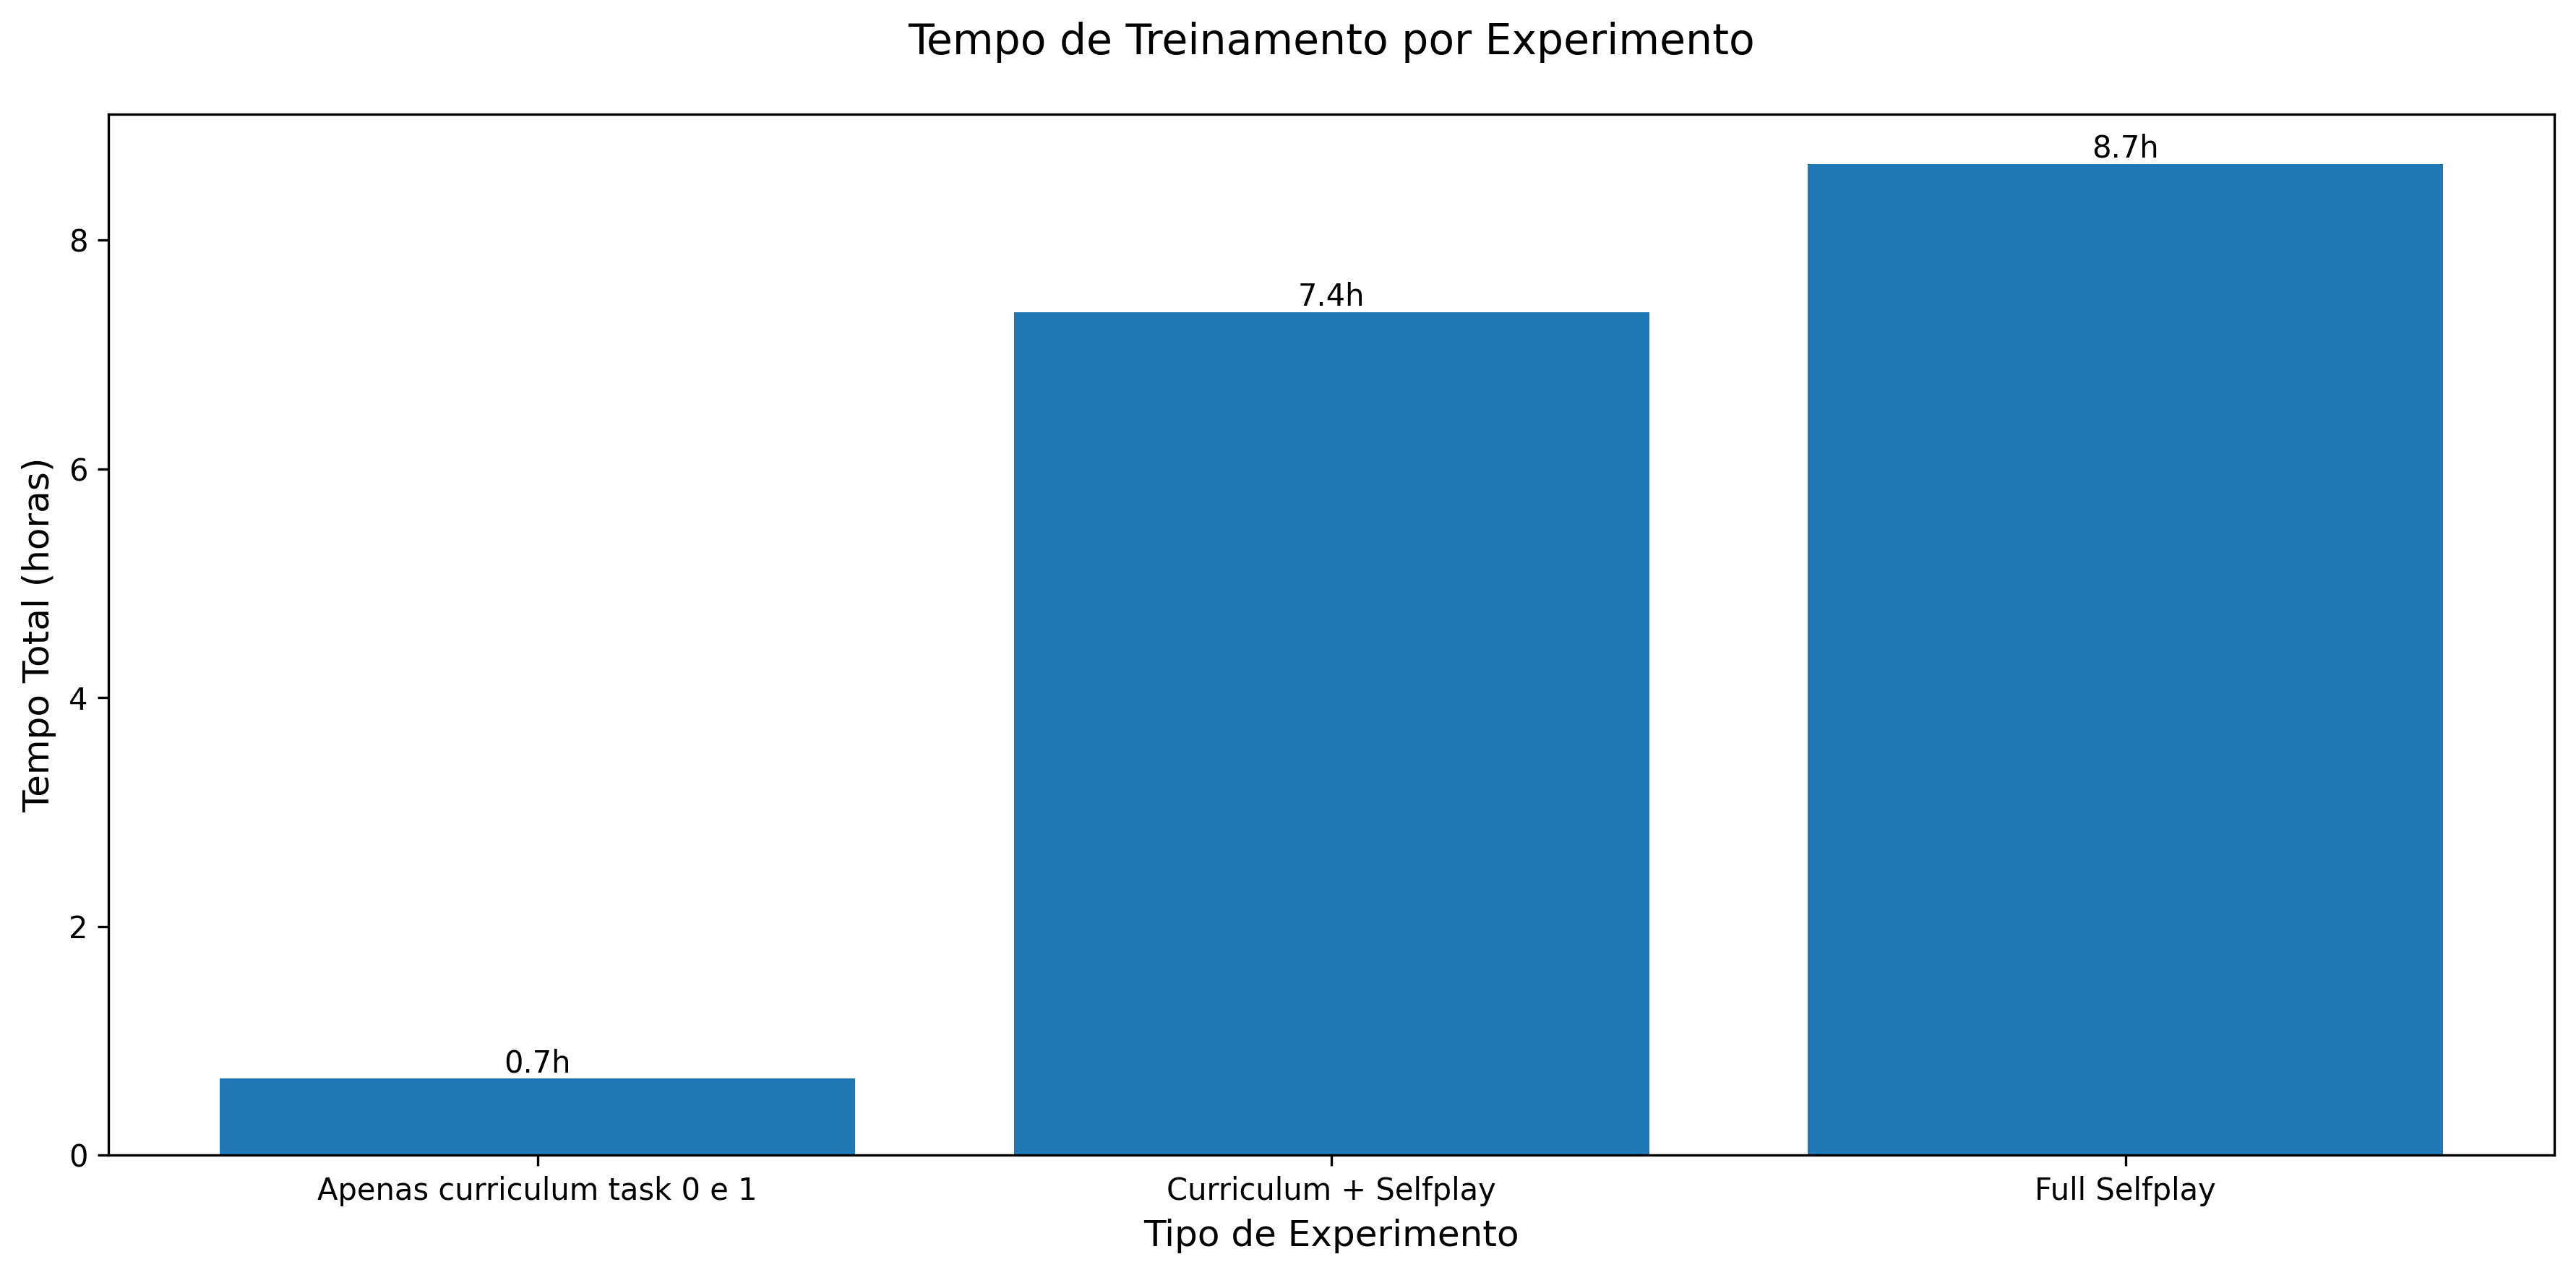
\includegraphics[width=0.9\textwidth]{fig/graficos_trabalho/graficos_experimentos/graficos_tempo_treino/tempo_treinamento.png}
    \caption{Comparação do tempo total de treinamento em horas para cada abordagem experimental}
    \label{fig:tempo_treinamento}
\end{figure}

A análise dos tempos de treinamento revela diferenças significativas entre as abordagens:

\begin{itemize}
    \item \textbf{Apenas \textit{curriculum} (\textit{tasks} 0 e 1)}: Aproximadamente 0,7 horas (42 minutos)
    \item \textbf{\textit{Curriculum} + \textit{Self-play}}: Aproximadamente 7,4 horas
    \item \textbf{\textit{Full Self-play}}: Aproximadamente 8,7 horas
\end{itemize}

Estas diferenças nos tempos de treinamento refletem a complexidade e a natureza de cada abordagem. O treinamento exclusivo com \textit{curriculum tasks} é significativamente mais rápido, pois envolve ambientes mais simples e objetivos bem definidos. A abordagem combinada (\textit{curriculum} + \textit{self-play}) apresenta um tempo de treinamento aproximadamente 15\% menor em relação ao \textit{full self-play} tradicional.

Esta economia de tempo é uma observação particularmente relevante do ponto de vista prático, especialmente considerando que a abordagem combinada também proporcionou resultados superiores (conforme demonstrado nas seções posteriores). Esta vantagem em termos de eficiência computacional representa um aspecto importante para aplicações práticas, onde os recursos de processamento são frequentemente limitados.

A maior eficiência da abordagem combinada pode ser atribuída ao fato de que as habilidades fundamentais desenvolvidas durante o \textit{curriculum} permitem que o agente aproveite melhor a fase de \textit{self-play}, convergindo mais rapidamente para políticas efetivas. Os agentes que iniciam diretamente no \textit{self-play} gastam mais tempo em fases iniciais de exploração aleatória, necessitando de iterações adicionais para desenvolver as mesmas capacidades que são adquiridas de forma estruturada no \textit{curriculum}.

\section{Análise Comparativa}
\label{sec:analise_comparativa}

Para avaliar a eficácia da abordagem proposta, realizamos uma análise comparativa entre o modelo treinado apenas com \textit{self-play} (\textit{baseline}) e o modelo treinado com a combinação de \textit{curriculum learning} e \textit{self-play} (modelo proposto). Esta análise abrange diversas métricas relevantes para o domínio do futebol de robôs.

\subsection{Evolução da Recompensa}

A análise da evolução da recompensa média ao longo do treinamento oferece \textit{insights} valiosos sobre o processo de aprendizagem dos agentes. A Figura \ref{fig:episode_reward} apresenta esta evolução para ambas as abordagens.

\begin{figure}[H]
    \centering
    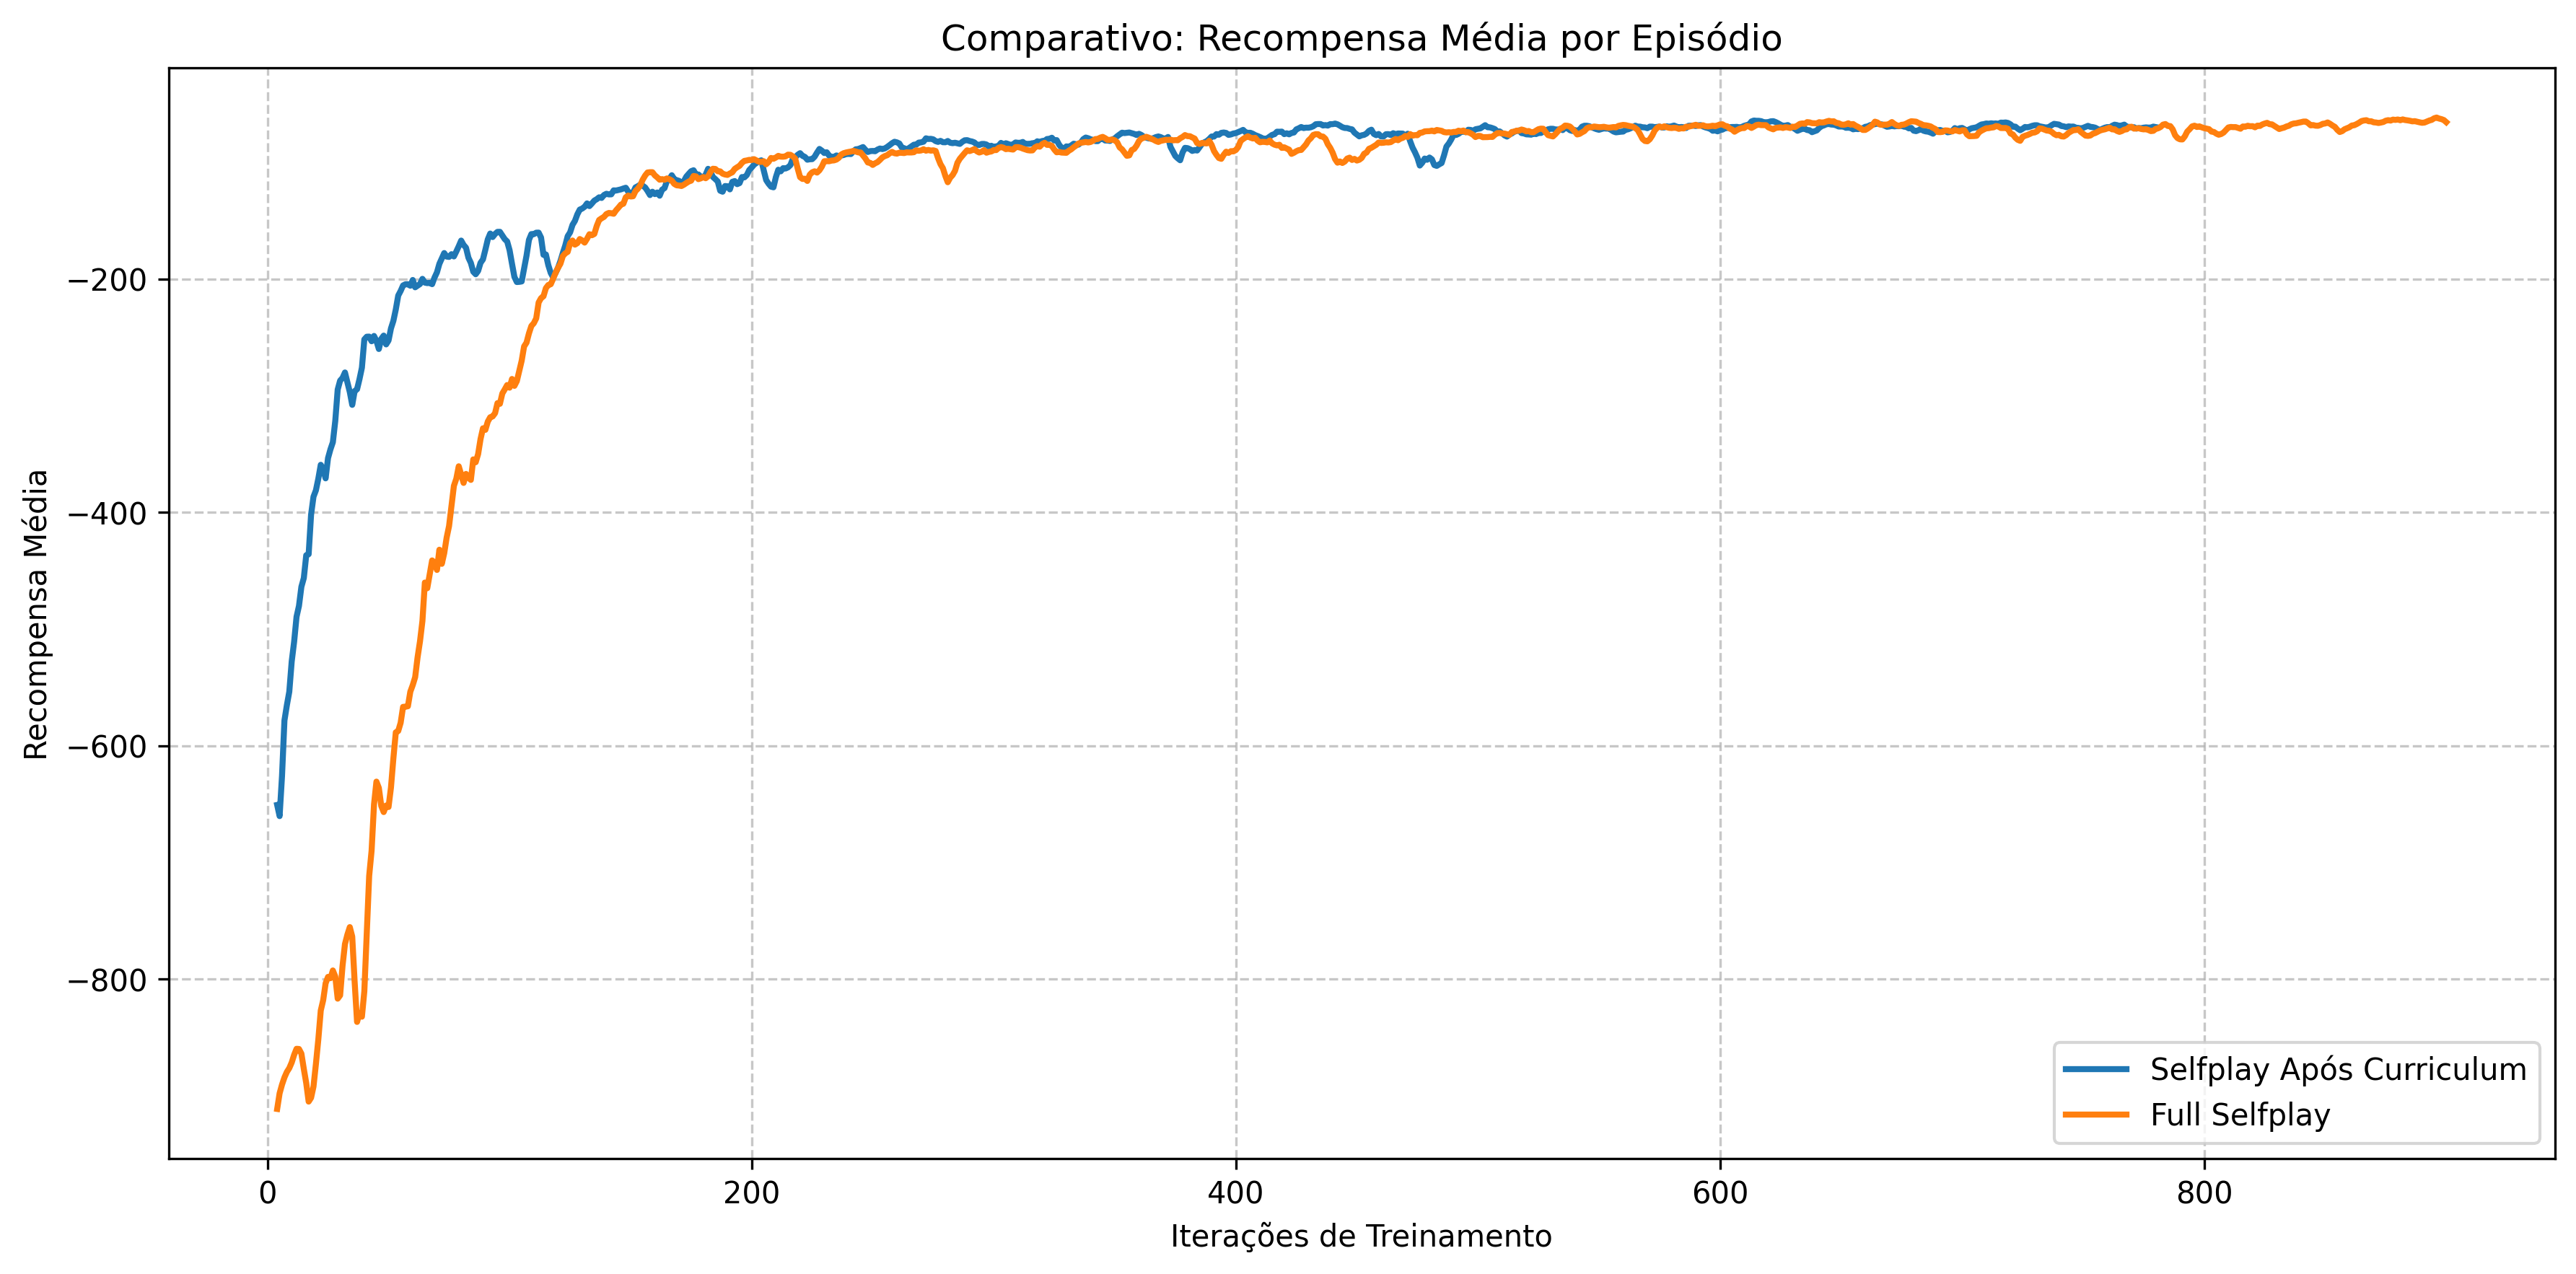
\includegraphics[width=0.8\textwidth]{fig/graficos_trabalho/graficos_experimentos/geral/comparativo_recompensa_media.png}
    \caption{Evolução da recompensa média por episódio ao longo do treinamento}
    \label{fig:episode_reward}
\end{figure}

O gráfico revela que o modelo treinado com \textit{curriculum learning} apresenta um crescimento mais acelerado da recompensa nas fases iniciais do treinamento. Esta vantagem inicial é atribuída à aprendizagem estruturada de habilidades fundamentais durante os estágios do \textit{curriculum}. Embora ambas as abordagens apresentem convergência em termos de recompensa acumulada, o modelo proposto atinge níveis equivalentes com menos \textit{timesteps} de treinamento, sugerindo maior eficiência no processo de aprendizagem.

Nota-se também que o modelo proposto apresenta menor variabilidade na curva de recompensa, indicando maior estabilidade durante o processo de treinamento.

Para compreender melhor como as habilidades fundamentais são desenvolvidas durante o \textit{curriculum}, é interessante analisar a evolução da recompensa em cada estágio específico. As Figuras \ref{fig:reward_task0} e \ref{fig:reward_task1} apresentam esta evolução para os estágios \textit{Task} 0 e \textit{Task} 1, respectivamente.

\begin{figure}[H]
    \centering
    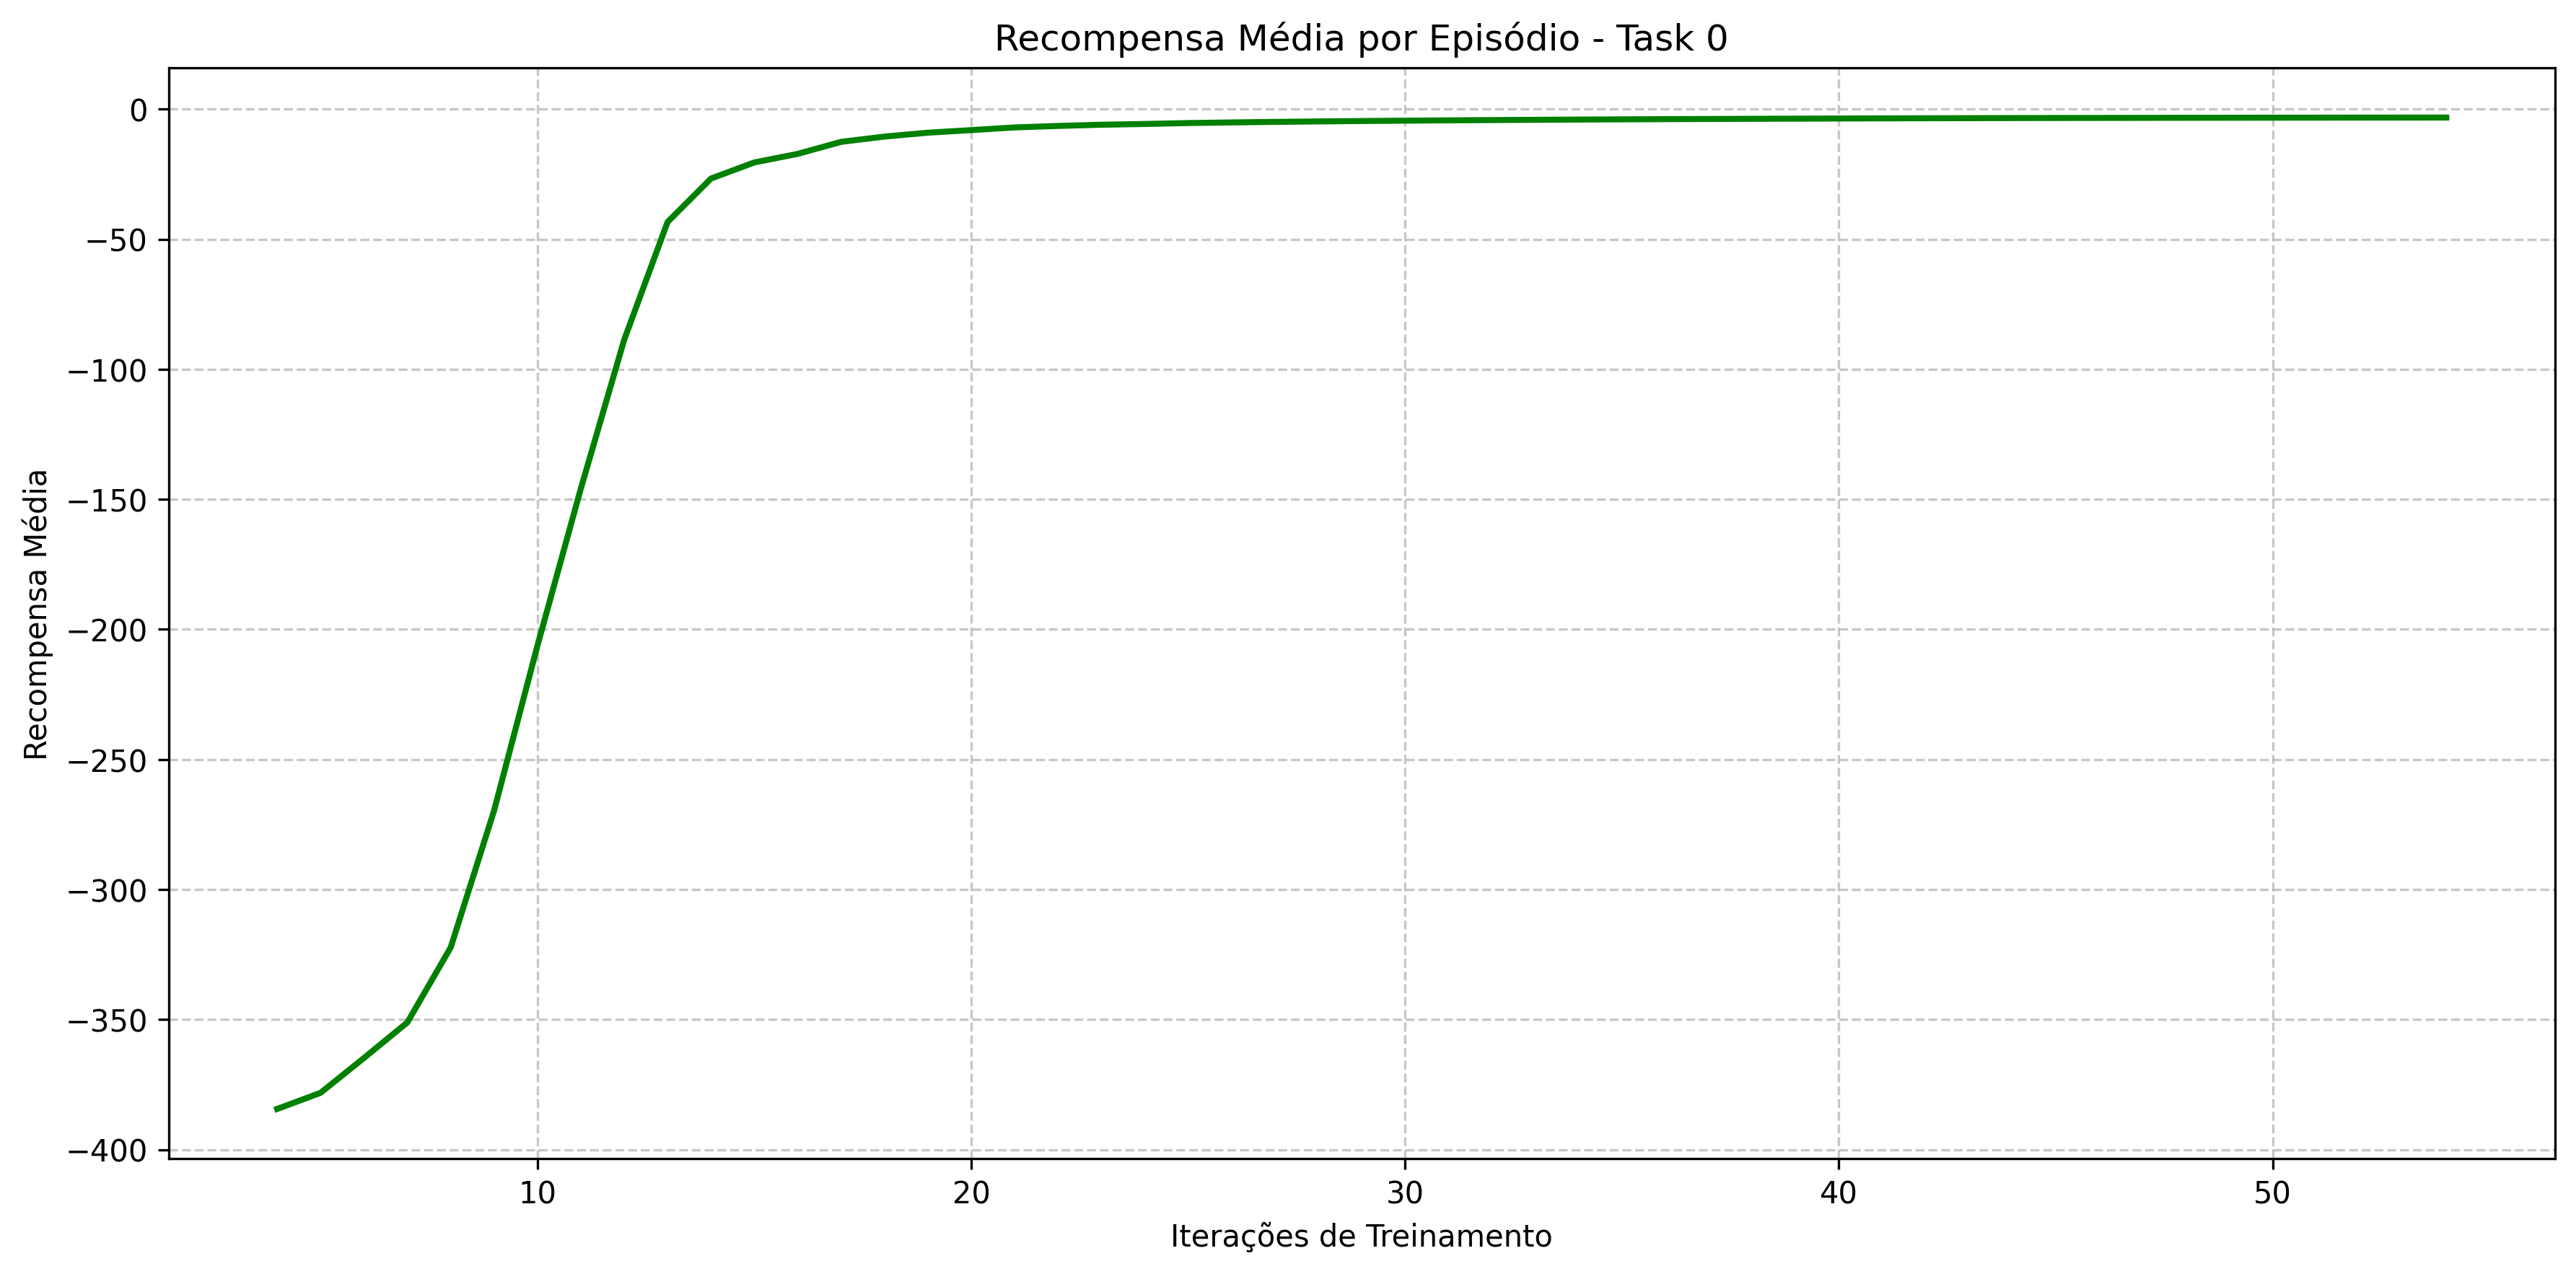
\includegraphics[width=0.8\textwidth]{fig/graficos_trabalho/graficos_experimentos/geral/recompensa_media_curriculum_task_0.png}
    \caption{Evolução da recompensa média por episódio durante o \textit{Curriculum Task} 0}
    \label{fig:reward_task0}
\end{figure}

\begin{figure}[H]
    \centering
    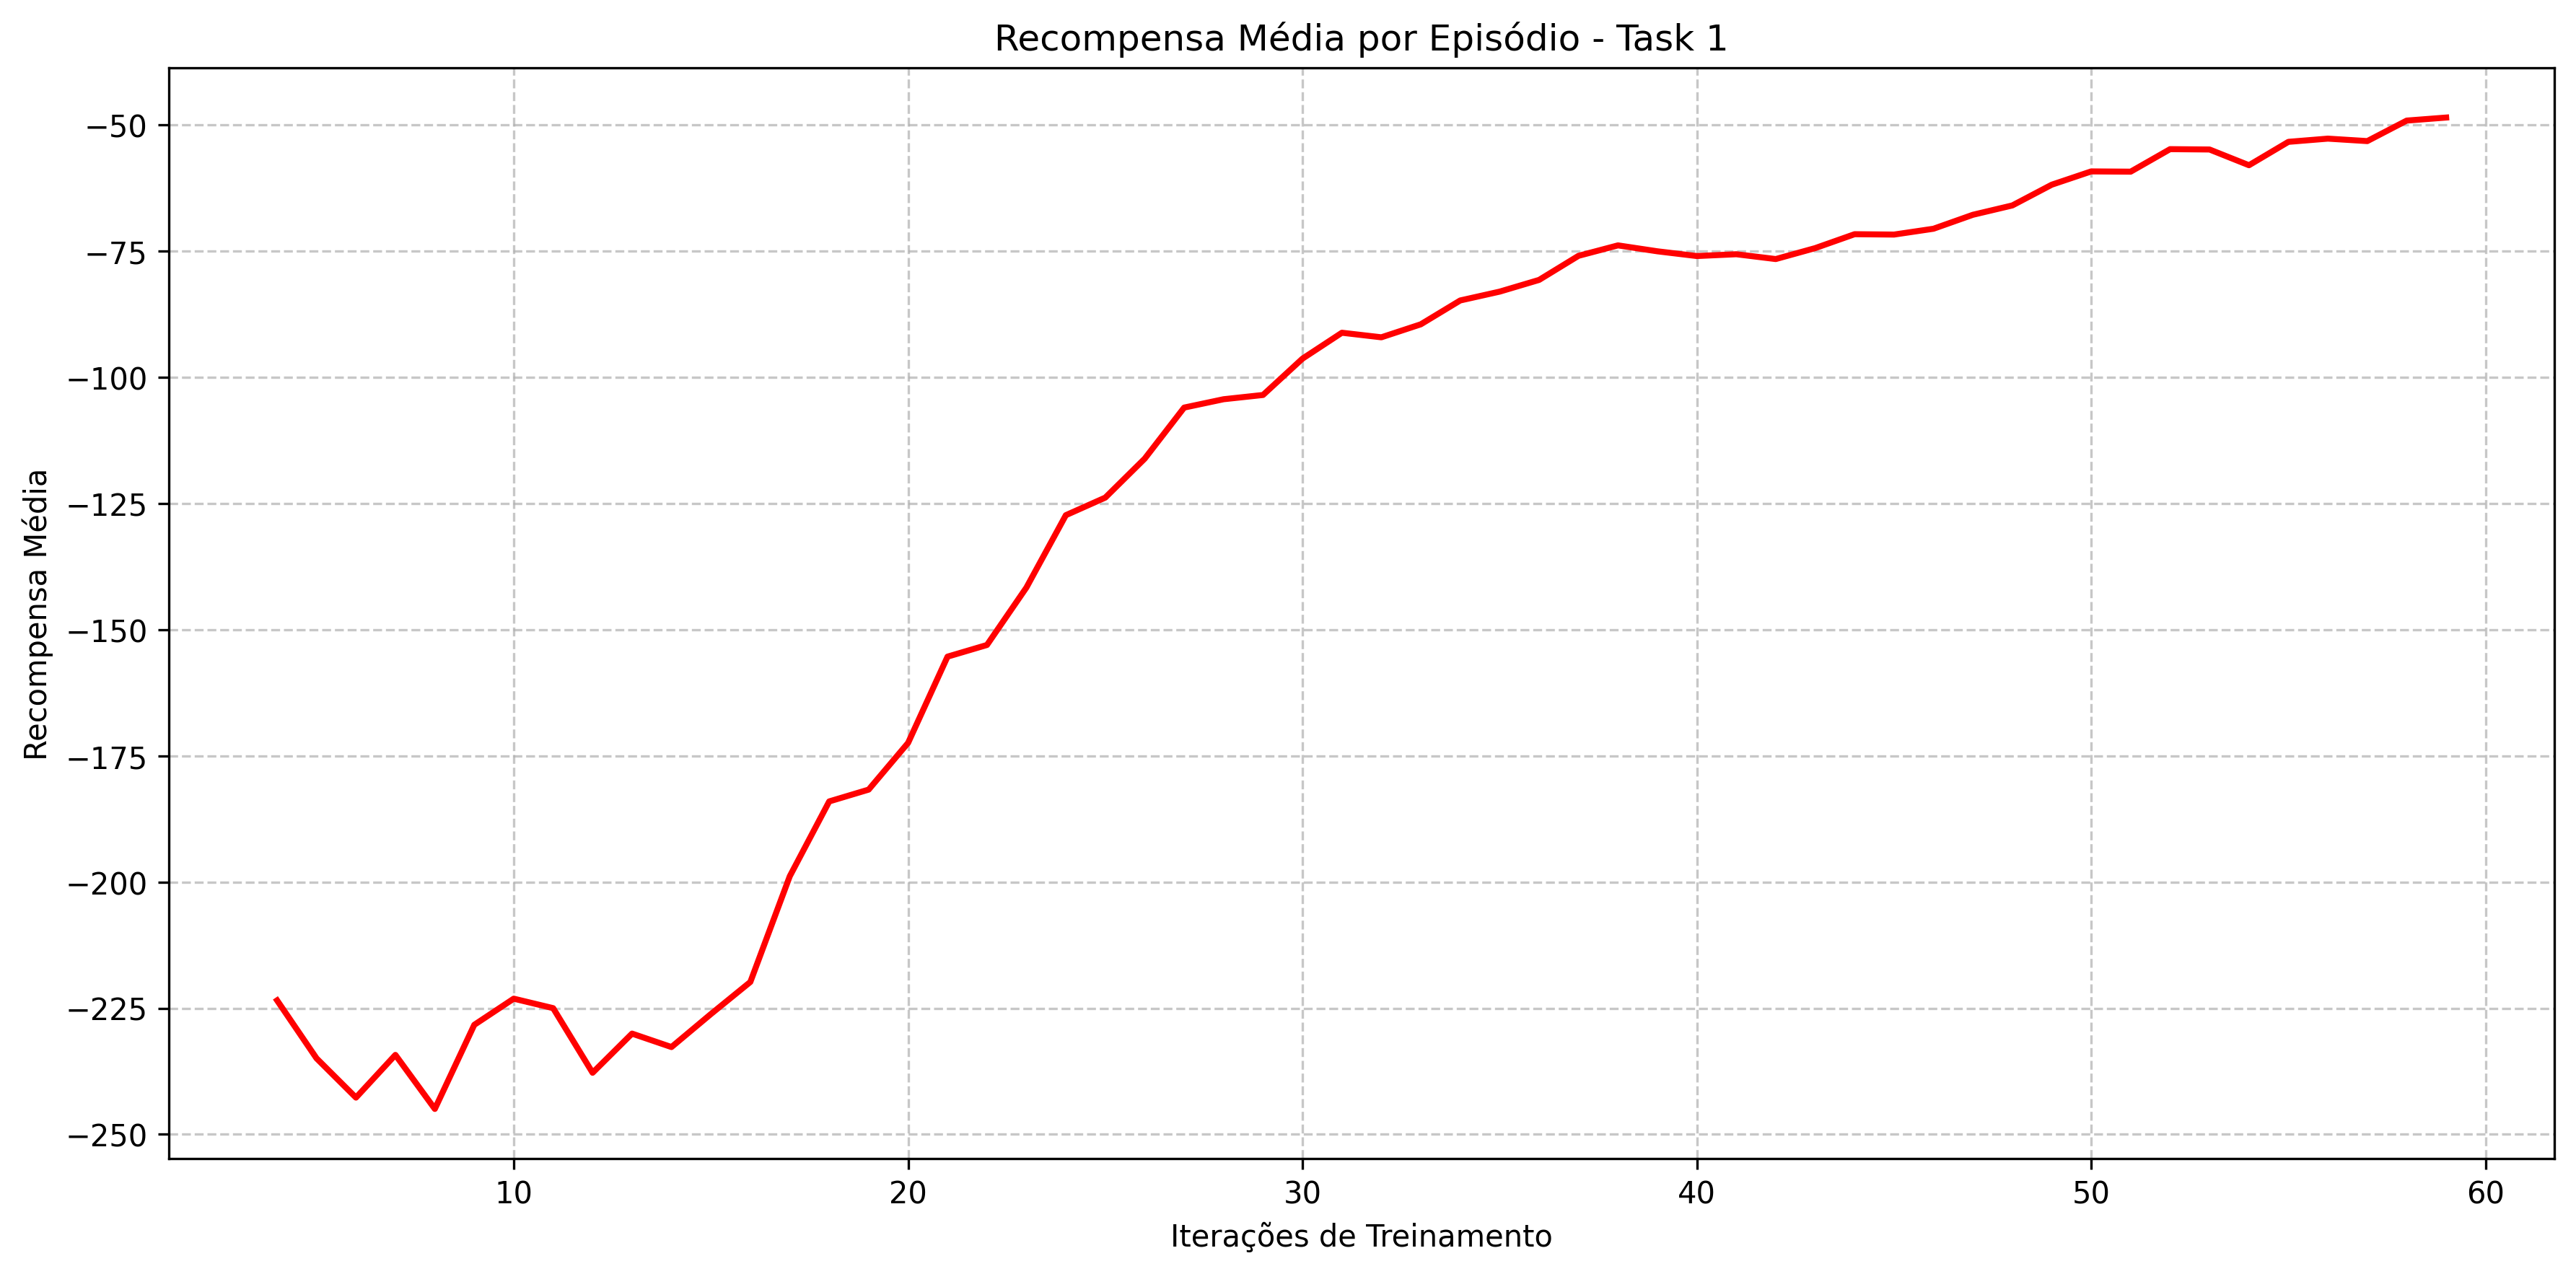
\includegraphics[width=0.8\textwidth]{fig/graficos_trabalho/graficos_experimentos/geral/recompensa_media_curriculum_task_1.png}
    \caption{Evolução da recompensa média por episódio durante o \textit{Curriculum Task} 1}
    \label{fig:reward_task1}
\end{figure}

Estes gráficos revelam padrões distintos de aprendizado em cada estágio do \textit{curriculum}. No \textit{Task} 0 (Figura \ref{fig:reward_task0}), observa-se um crescimento acentuado da recompensa nas primeiras 15 iterações, partindo de valores próximos a -400 e estabilizando rapidamente em torno de 0. Esta evolução demonstra que os agentes aprendem eficientemente as habilidades básicas de controle e aproximação da bola, atingindo o critério de promoção em poucas iterações.

Já no \textit{Task} 1 (Figura \ref{fig:reward_task1}), nota-se um padrão de aprendizado mais gradual e complexo. A curva apresenta oscilações iniciais entre as iterações 5 e 15, seguidas por um crescimento consistente até a iteração 60, quando a recompensa média atinge aproximadamente -50. Este comportamento reflete a maior complexidade desta tarefa, que exige coordenação entre múltiplos agentes e estratégias ofensivas mais sofisticadas na presença de oponentes estáticos.

A comparação entre estes dois estágios ilustra claramente a progressão de complexidade no \textit{curriculum} e como os agentes desenvolvem diferentes habilidades em cada fase. O rápido progresso no \textit{Task} 0 estabelece a base motora fundamental, enquanto o aprendizado mais gradual no \textit{Task} 1 desenvolve capacidades táticas e coordenativas que serão cruciais durante o posterior treinamento com \textit{self-play}.

\subsection{Desempenho Ofensivo}

O desempenho ofensivo dos agentes foi avaliado principalmente através da análise da taxa de sucesso na conclusão dos objetivos. A Figura \ref{fig:goals_blue_comparison} apresenta a evolução desta métrica ao longo do treinamento para ambas as abordagens.

\begin{figure}[H]
    \centering
    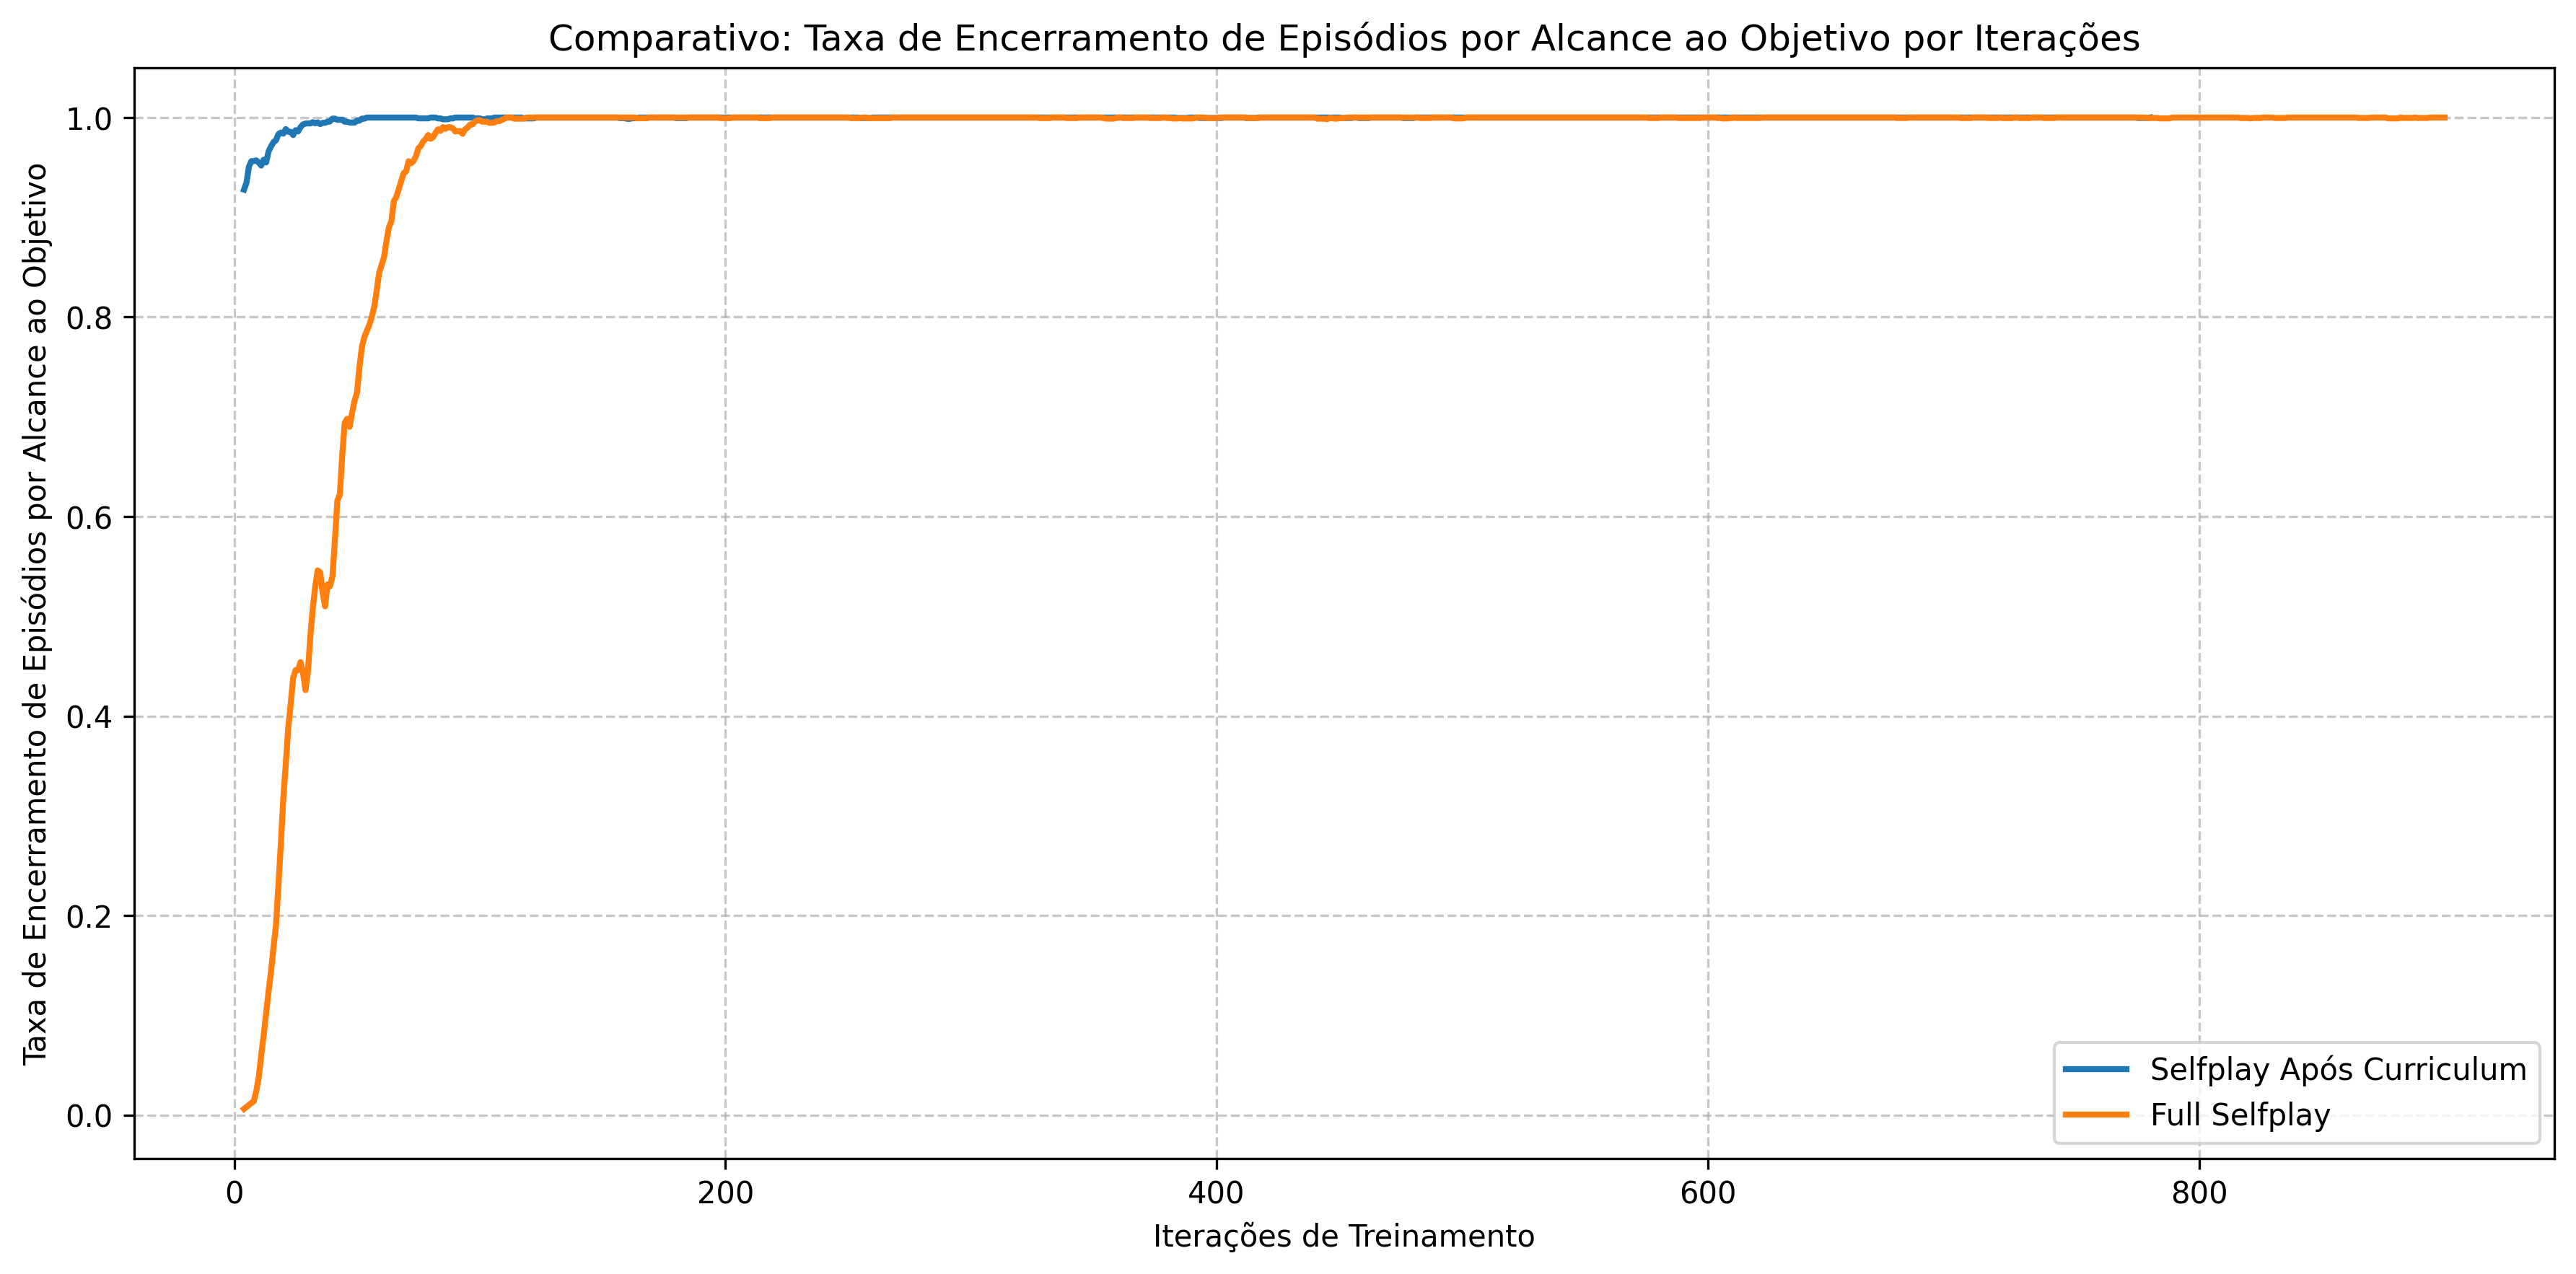
\includegraphics[width=0.95\textwidth]{fig/graficos_trabalho/graficos_experimentos/geral/comparativo_taxa_encerramento_episodios.png}
    \caption{Comparativo: Taxa de Encerramento de Episódios por Alcance ao Objetivo por Iterações entre as abordagens \textit{Selfplay} após \textit{Curriculum} e \textit{Full Selfplay}}
    \label{fig:goals_blue_comparison}
\end{figure}

A análise comparativa do gráfico revela padrões interessantes na evolução da capacidade dos agentes de atingir seus objetivos. Ambas as abordagens apresentam uma progressão crescente na taxa de sucesso, eventualmente atingindo valores próximos a 100\%. No entanto, observam-se diferenças significativas no processo de aprendizado:

\begin{itemize}
    \item \textbf{Velocidade de convergência}: O \textit{Selfplay} após \textit{Curriculum} (linha azul) atinge o patamar próximo a 100\% de sucesso muito mais rapidamente, convergindo nas primeiras 50 iterações, enquanto o \textit{Full Selfplay} (linha laranja) requer cerca de 150 iterações para alcançar desempenho semelhante.
    
    \item \textbf{Fase inicial}: Nas primeiras iterações, o \textit{Selfplay} após \textit{Curriculum} já começa com uma taxa de sucesso em torno de 90\%, demonstrando que as habilidades adquiridas durante a fase de \textit{curriculum} proporcionam um ponto de partida significativamente mais avançado.
    
    \item \textbf{Estabilidade}: Ambas as abordagens eventualmente atingem estabilidade, mas o \textit{Selfplay} após \textit{Curriculum} apresenta menor variabilidade durante todo o processo, indicando um aprendizado mais consistente e robusto.
\end{itemize}

Esta comparação com iterações alinhadas evidencia de forma clara uma vantagem significativa da abordagem proposta: ao iniciar o \textit{self-play} com agentes já treinados em tarefas fundamentais através do \textit{curriculum}, obtém-se uma aceleração substancial na capacidade de atingir objetivos. Esta característica é particularmente valiosa em cenários com restrições de tempo computacional, onde a convergência mais rápida para políticas de alta qualidade representa uma vantagem considerável.

\subsection{Eficiência e Continuidade do Jogo}

No contexto deste trabalho, um \textit{reset} representa o reposicionamento dos robôs às suas posições iniciais, ocorrendo sempre que a bola sai do campo. Este reposicionamento é necessário para garantir a continuidade da partida.

Um aspecto diferencial da abordagem proposta é a melhoria significativa nas métricas relacionadas à continuidade do jogo, que refletem a capacidade dos agentes de manter a bola em jogo por períodos mais longos. A Figura \ref{fig:total_resets} apresenta a evolução do número médio de \textit{resets} por episódio.

\begin{figure}[H]
    \centering
    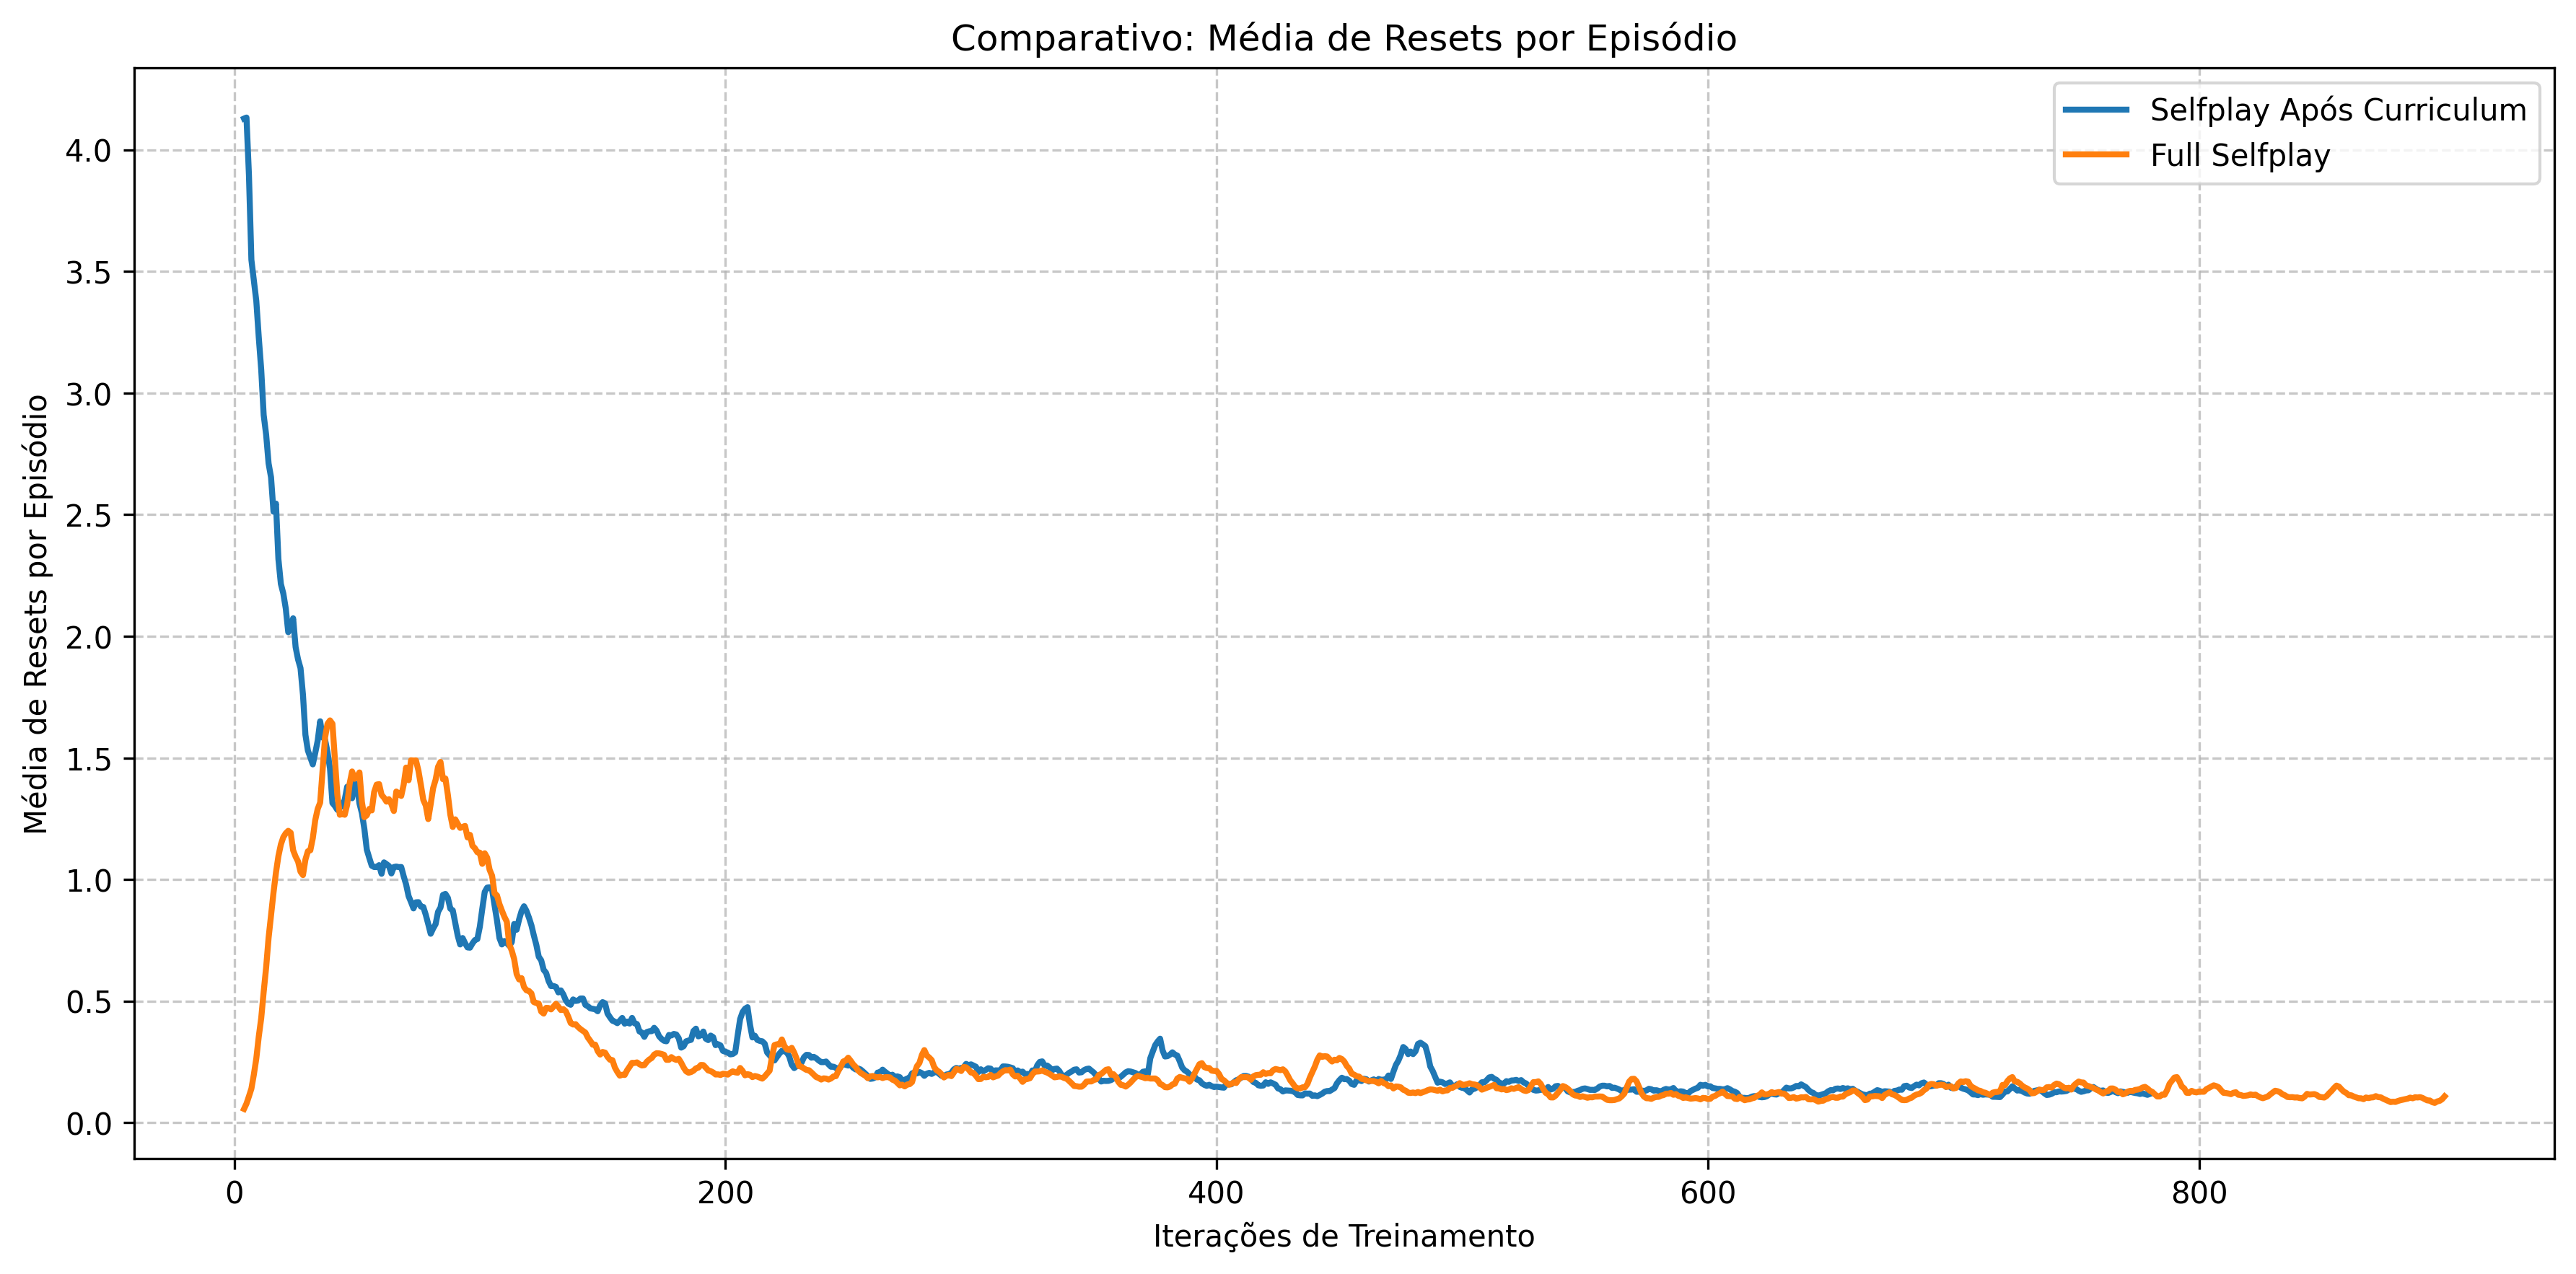
\includegraphics[width=0.95\textwidth]{fig/graficos_trabalho/graficos_experimentos/geral/comparativo_resets_por_episodio.png}
    \caption{Comparativo da média de \textit{resets} por episódio: \textit{Selfplay} após \textit{Curriculum} e \textit{Full Selfplay}}
    \label{fig:total_resets}
\end{figure}

A análise do gráfico revela diferenças significativas nos padrões de aprendizado relacionados à continuidade do jogo. Inicialmente, o \textit{Selfplay} após \textit{Curriculum} (linha azul) apresenta um pico maior de \textit{resets} por episódio, mas rapidamente consegue reduzir esse número. O \textit{Full Selfplay} (linha laranja) mostra um comportamento diferente, com um aumento gradual seguido por uma redução mais lenta.

Após aproximadamente 200 iterações, ambas as abordagens convergem para valores similares, com ligeira vantagem para o \textit{Full Selfplay} nas iterações finais. No entanto, é notável que o \textit{Selfplay} após \textit{Curriculum} consegue reduzir o número de \textit{resets} de forma mais rápida nas fases iniciais do treinamento, evidenciando a transferência positiva das habilidades adquiridas durante o \textit{curriculum}.

Esta análise demonstra que, embora ambas as abordagens eventualmente atinjam desempenhos similares em termos de continuidade do jogo em suas fases finais, o \textit{Selfplay} após \textit{Curriculum} oferece um processo de aprendizado mais eficiente e estável, especialmente durante as fases iniciais e intermediárias do treinamento.

\subsection{Duração dos Episódios}

A análise da duração média dos episódios ao longo do treinamento (Figura \ref{fig:episode_len}) revela padrões interessantes sobre a evolução das estratégias desenvolvidas pelos agentes.

\begin{figure}[H]
    \centering
    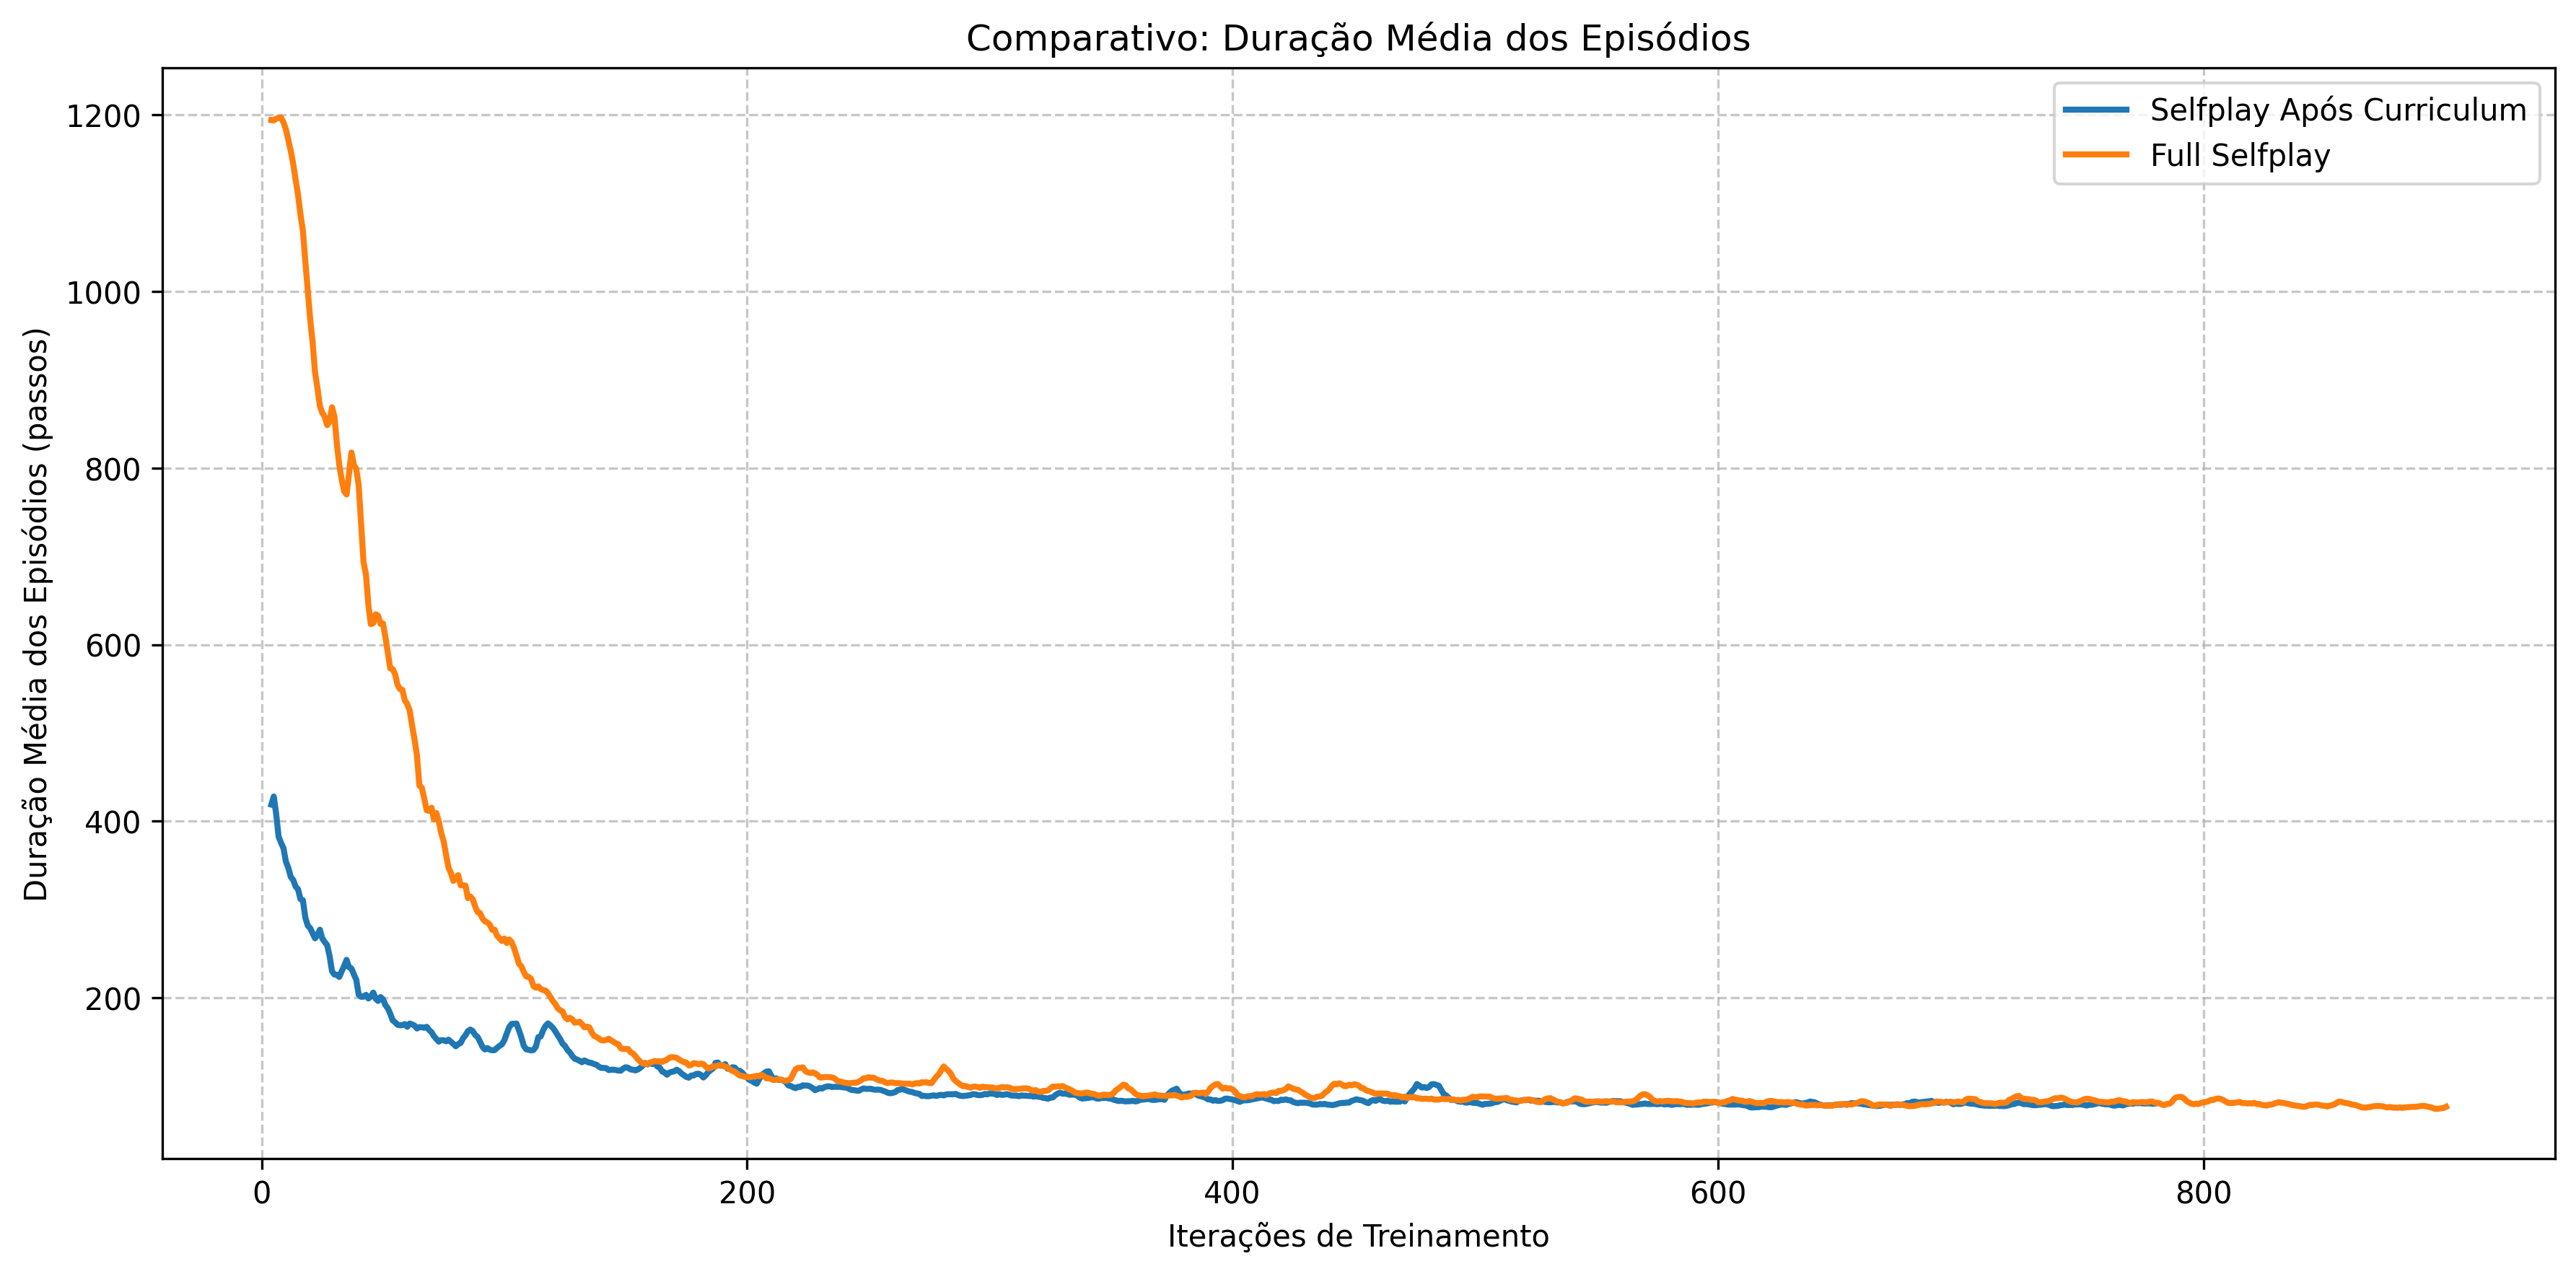
\includegraphics[width=0.95\textwidth]{fig/graficos_trabalho/graficos_experimentos/geral/comparativo_duracao_episodios.png}
    \caption{Comparativo da duração média dos episódios: \textit{Selfplay} após \textit{Curriculum} e \textit{Full Selfplay}}
    \label{fig:episode_len}
\end{figure}

A análise do gráfico revela diferenças marcantes no comportamento dos agentes em relação à duração dos episódios. O \textit{Full Selfplay} (linha laranja) inicia com episódios significativamente mais longos, atingindo aproximadamente 1200 passos nas primeiras iterações, enquanto o \textit{Selfplay} após \textit{Curriculum} (linha azul) começa com episódios bem mais curtos, em torno de 400 passos. Esta diferença inicial demonstra que as habilidades adquiridas durante as fases de \textit{curriculum} proporcionam um ponto de partida mais eficiente, permitindo aos agentes atingir seus objetivos em menos passos desde o início.

Ao longo do treinamento, ambas as abordagens apresentam uma redução gradual na duração dos episódios, convergindo para valores similares após aproximadamente 200 iterações, quando estabilizam em torno de 100 passos por episódio. Esta redução na duração dos episódios é um indicador positivo, pois demonstra que os agentes estão se tornando mais eficientes em marcar gols, já que cada episódio é encerrado quando um gol é marcado. É notável que o \textit{Selfplay} após \textit{Curriculum} apresenta uma curva de aprendizado mais suave e consistente, sem as oscilações pronunciadas observadas no \textit{Full Selfplay}, indicando um processo de aprendizagem mais estável e uma evolução mais consistente na capacidade de finalização. Nas iterações finais, ambas as abordagens mantêm desempenho similar em termos de velocidade para marcar gols, mas o caminho percorrido pelo \textit{Selfplay} após \textit{Curriculum} para atingir este patamar demonstra maior eficiência, especialmente nas fases críticas iniciais e intermediárias do treinamento.

\subsection{Avaliação por Torneios}

Para uma avaliação mais abrangente e realista do desempenho dos modelos treinados, foram realizados torneios controlados com 500 partidas cada, utilizando o sistema \textit{Arena Serra Dourada}, implementado especificamente para este trabalho. Este sistema permitiu a realização de partidas completas com 10 minutos de duração entre agentes treinados por diferentes métodos.

Os torneios foram organizados em dois confrontos distintos:
\begin{itemize}
    \item \textbf{Torneio 1}: \textit{Full Selfplay} vs \textit{Curriculum} - 500 partidas entre agentes treinados apenas com \textit{self-play} e agentes treinados apenas com \textit{curriculum learning}.
    \item \textbf{Torneio 2}: \textit{Full Selfplay} vs \textit{Curriculum} + \textit{Selfplay} - 500 partidas entre agentes treinados apenas com \textit{self-play} e agentes treinados com a abordagem combinada (\textit{curriculum} seguido por \textit{self-play}).
\end{itemize}

Cada partida tinha duração de 10 minutos e seguia as regras básicas semelhantes a do futebol de robôs, como contabilização de gols e \textit{resets}. Esta configuração experimental permitiu avaliar não apenas a eficácia em marcar gols, mas também a estabilidade das políticas aprendidas em jogos completos e a capacidade de adaptação a diferentes situações de jogo.

A Tabela \ref{tab:resultados_torneios} apresenta um resumo dos resultados dos dois torneios realizados.

\begin{table}[H]
    \centering
    \begin{tabular}{|c|c|c|c|c|c|}
        \hline
        \textbf{Torneio} & \textbf{Partidas} & \textbf{Equipe} & \textbf{Vitórias} & \textbf{Gols} & \textbf{Empates} \\
        \hline
        Torneio 1 & \multicolumn{1}{c|}{500} & \textit{Full Selfplay} & 247 (49,4\%) & 503 & \multicolumn{1}{c|}{220 (44\%)} \\
        \cline{3-5}
        & & \textit{Curriculum} & 33 (6,6\%) & 58 & \\
        \hline
        Torneio 2 & \multicolumn{1}{c|}{500} & \textit{Full Selfplay} & 7 (1,4\%) & 9 & \multicolumn{1}{c|}{63 (12,6\%)} \\
        \cline{3-5}
        & & \textit{Curriculum} + \textit{Selfplay} & 430 (86\%) & 1012 & \\
        \hline
    \end{tabular}
    \caption{Resumo dos resultados dos torneios realizados com 500 partidas cada}
    \label{tab:resultados_torneios}
\end{table}

Os resultados revelam padrões interessantes sobre o desempenho de cada abordagem. No Torneio 1 (\textit{Full Selfplay} vs \textit{Curriculum}), observamos uma clara superioridade do modelo treinado apenas com \textit{self-play}, que obteve 247 vitórias (49,4\%) contra apenas 33 vitórias (6,6\%) do modelo treinado somente com \textit{curriculum learning}. É notável também o alto número de empates (220, correspondendo a 44\% dos jogos), sugerindo que o modelo de \textit{curriculum}, apesar de seu desempenho inferior em termos de vitórias, desenvolveu capacidades defensivas significativas.

No Torneio 2 (\textit{Full Selfplay} vs \textit{Curriculum} + \textit{Selfplay}), os resultados evidenciam a acentuada superioridade do modelo treinado com a combinação de \textit{curriculum learning} e \textit{self-play}, que obteve 430 vitórias (86\%) em comparação com apenas 7 vitórias (1,4\%) do modelo \textit{full self-play}. O número de empates foi significativamente menor (63, apenas 12,6\% dos jogos), indicando partidas mais decisivas e menos equilibradas.

Esta diferença acentuada no desempenho destaca o poderoso resultado obtido ao combinar as duas abordagens. Enquanto o \textit{curriculum learning} isolado apresenta limitações significativas em um cenário competitivo completo, sua integração com o \textit{self-play} resulta em políticas substancialmente mais eficazes do que aquelas desenvolvidas apenas com \textit{self-play}.

\begin{figure}[H]
    \centering
    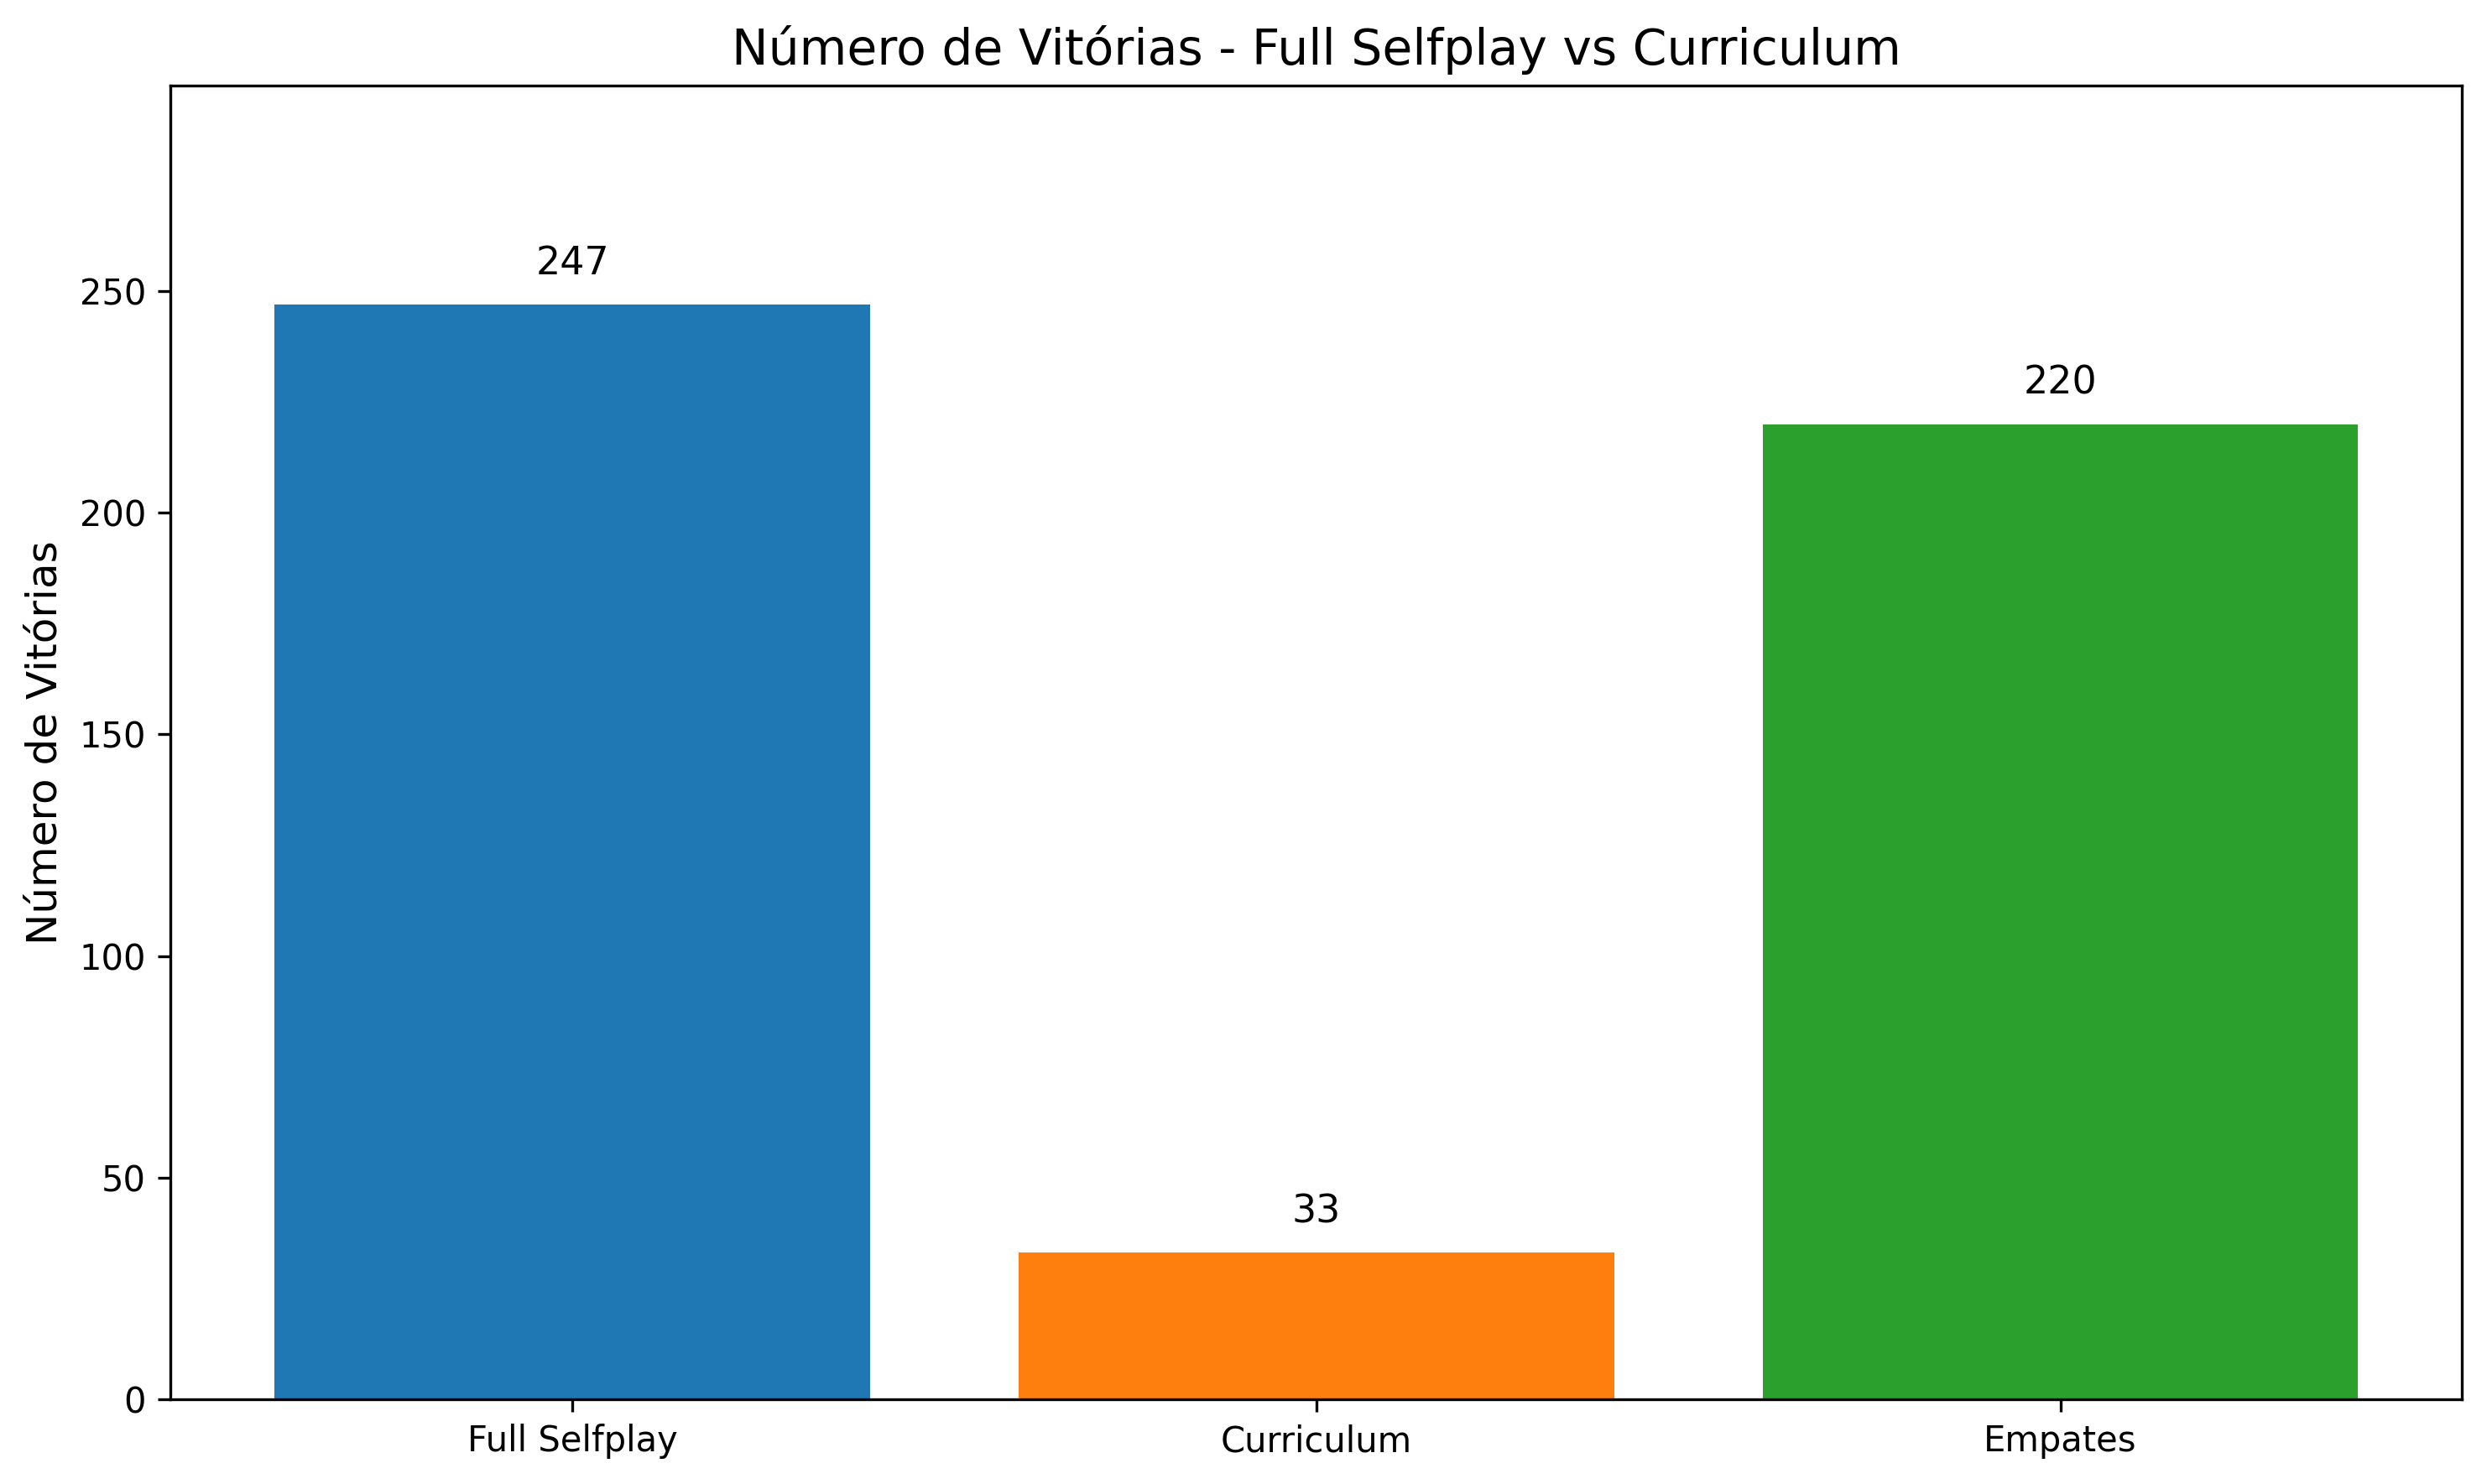
\includegraphics[width=0.8\textwidth]{fig/graficos_trabalho/graficos_torneios/torneios/vitorias_full_selfplay_vs_curriculum.png}
    \caption{Distribuição de resultados no Torneio 1: \textit{Full Selfplay} vs \textit{Curriculum}}
    \label{fig:vitorias_torneio1}
\end{figure}

\begin{figure}[H]
    \centering
    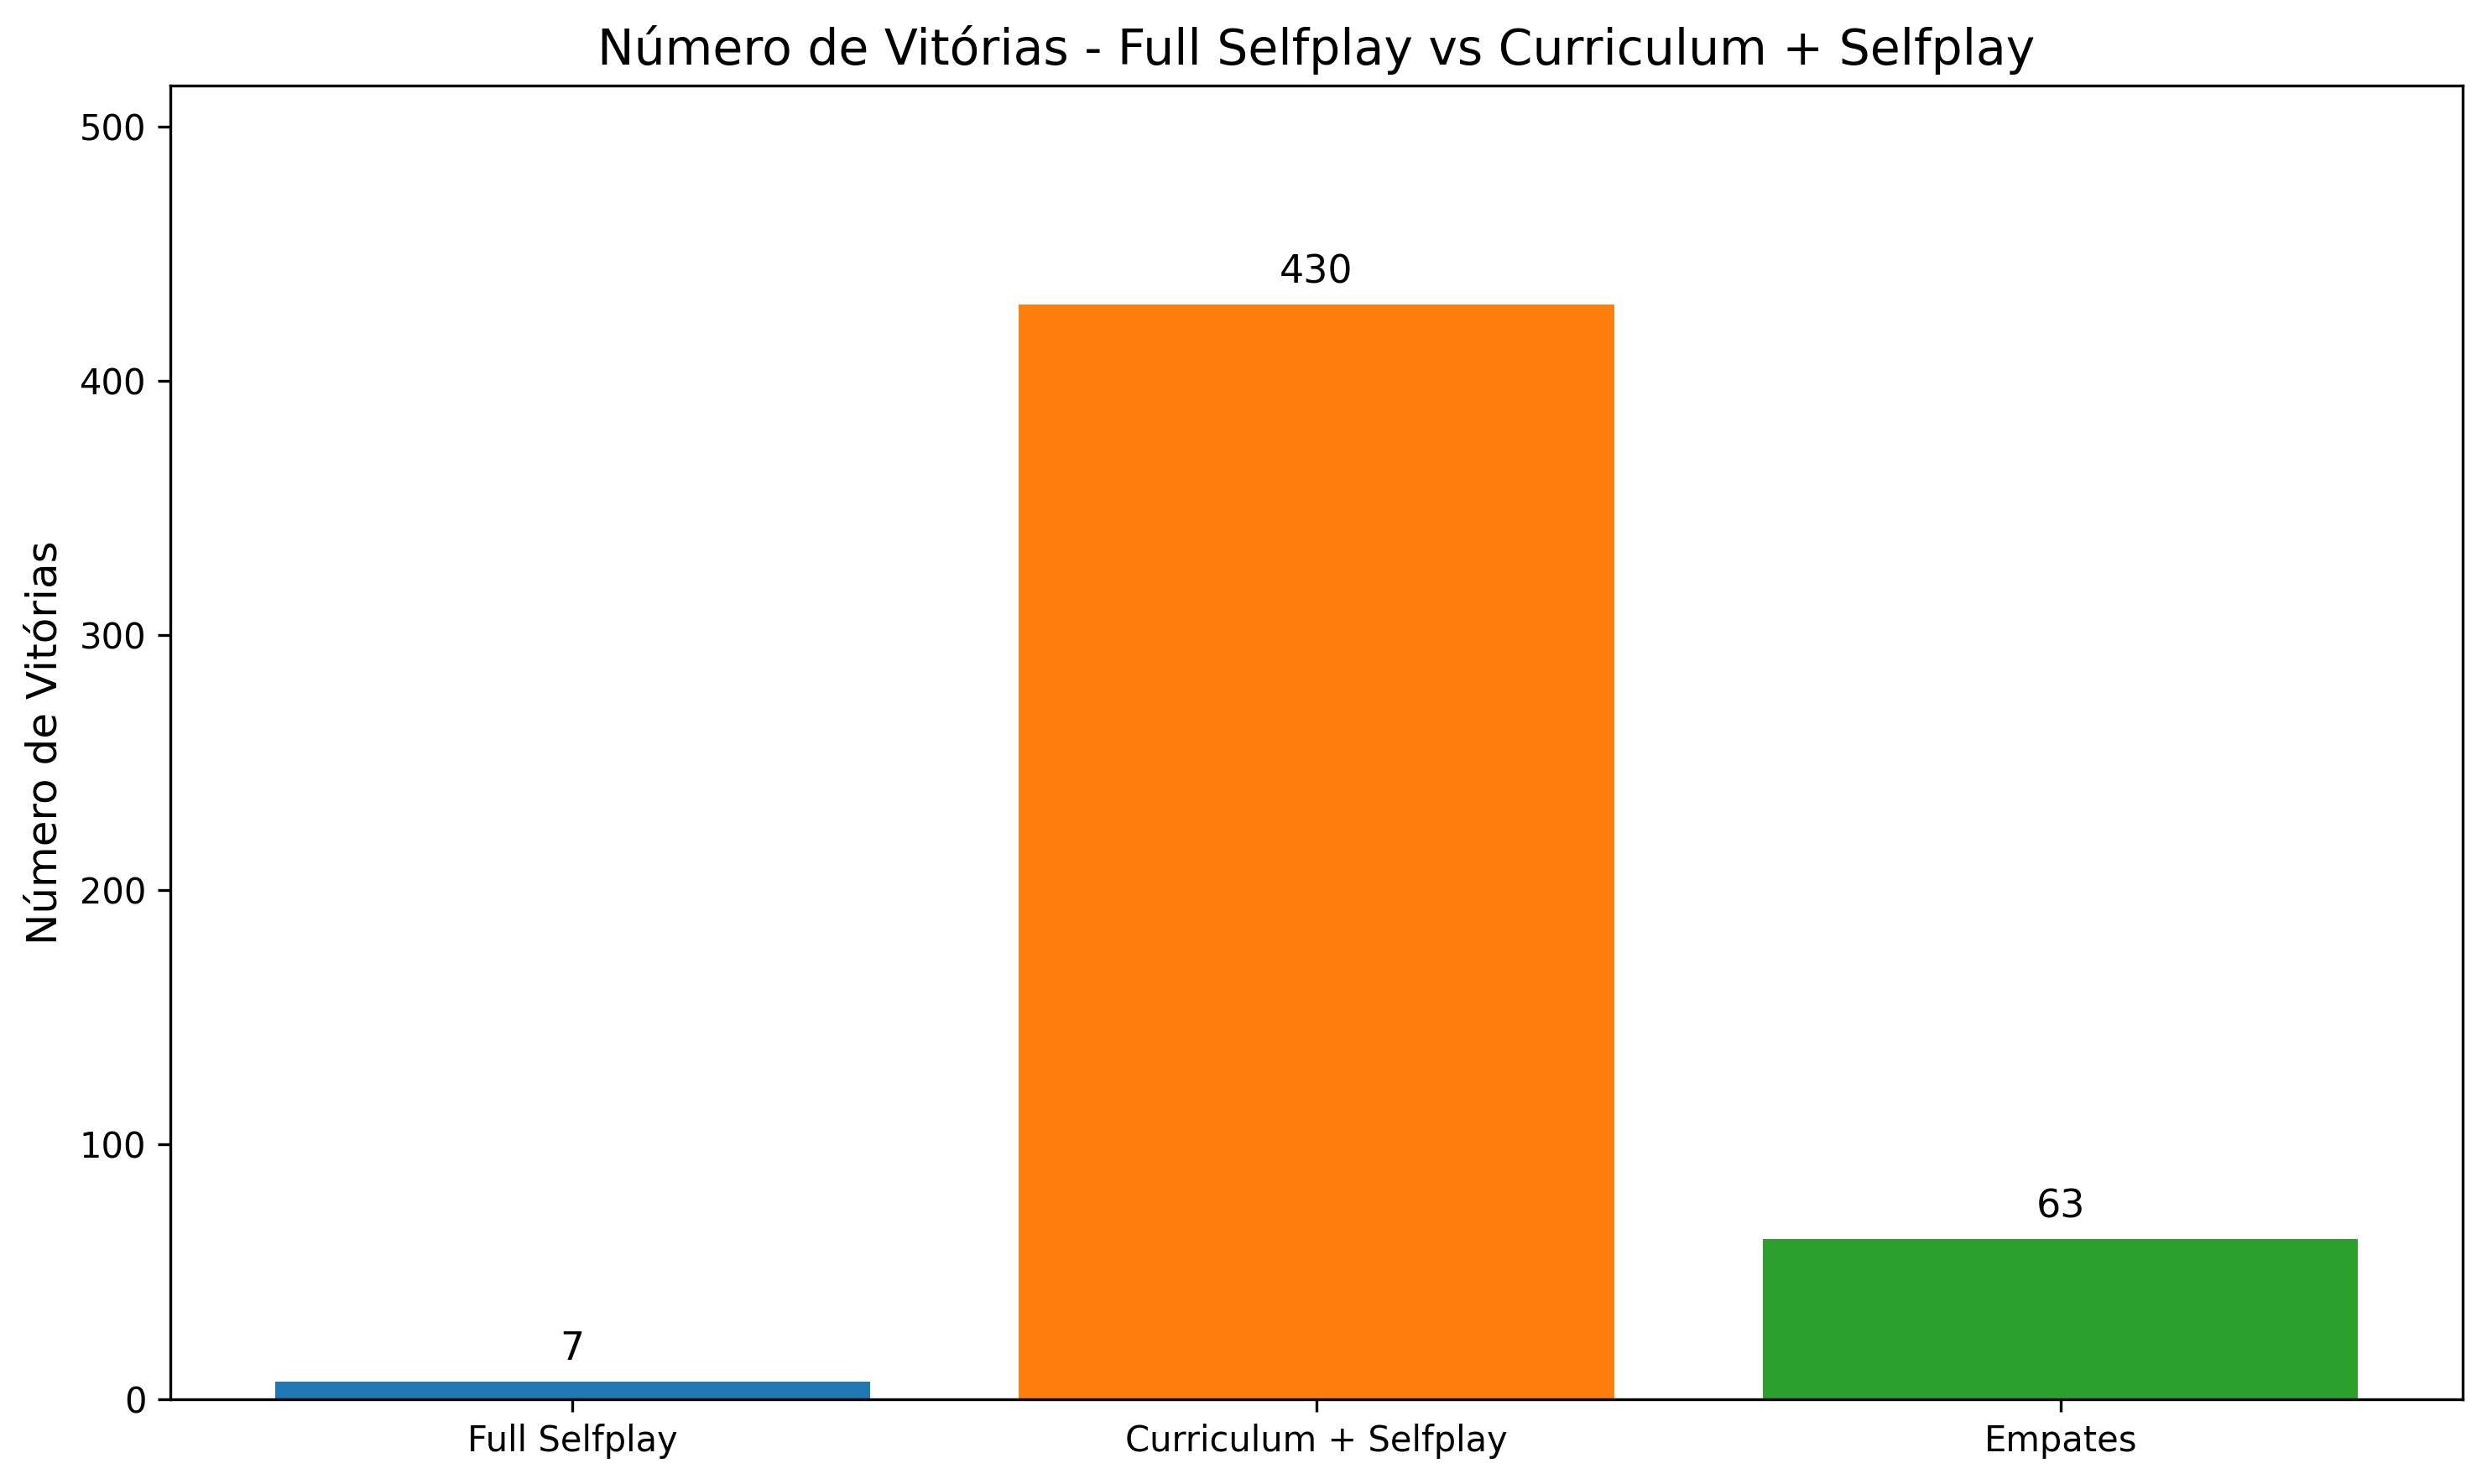
\includegraphics[width=0.8\textwidth]{fig/graficos_trabalho/graficos_torneios/torneios/vitorias_full_selfplay_vs_curriculum_+_selfplay.png}
    \caption{Distribuição de resultados no Torneio 2: \textit{Full Selfplay} vs \textit{Curriculum} + \textit{Selfplay}}
    \label{fig:vitorias_torneio2}
\end{figure}

A comparação visual das Figuras \ref{fig:vitorias_torneio1} e \ref{fig:vitorias_torneio2} evidencia claramente a inversão de desempenho entre os torneios e o impacto transformador da abordagem combinada.

\subsection{Análise de Gols nos Torneios}

Além da taxa de vitória, analisamos também o desempenho ofensivo dos modelos nos torneios realizados, com foco na capacidade de marcar gols, que representa um indicador fundamental de eficácia no futebol de robôs.

\begin{figure}[H]
    \centering
    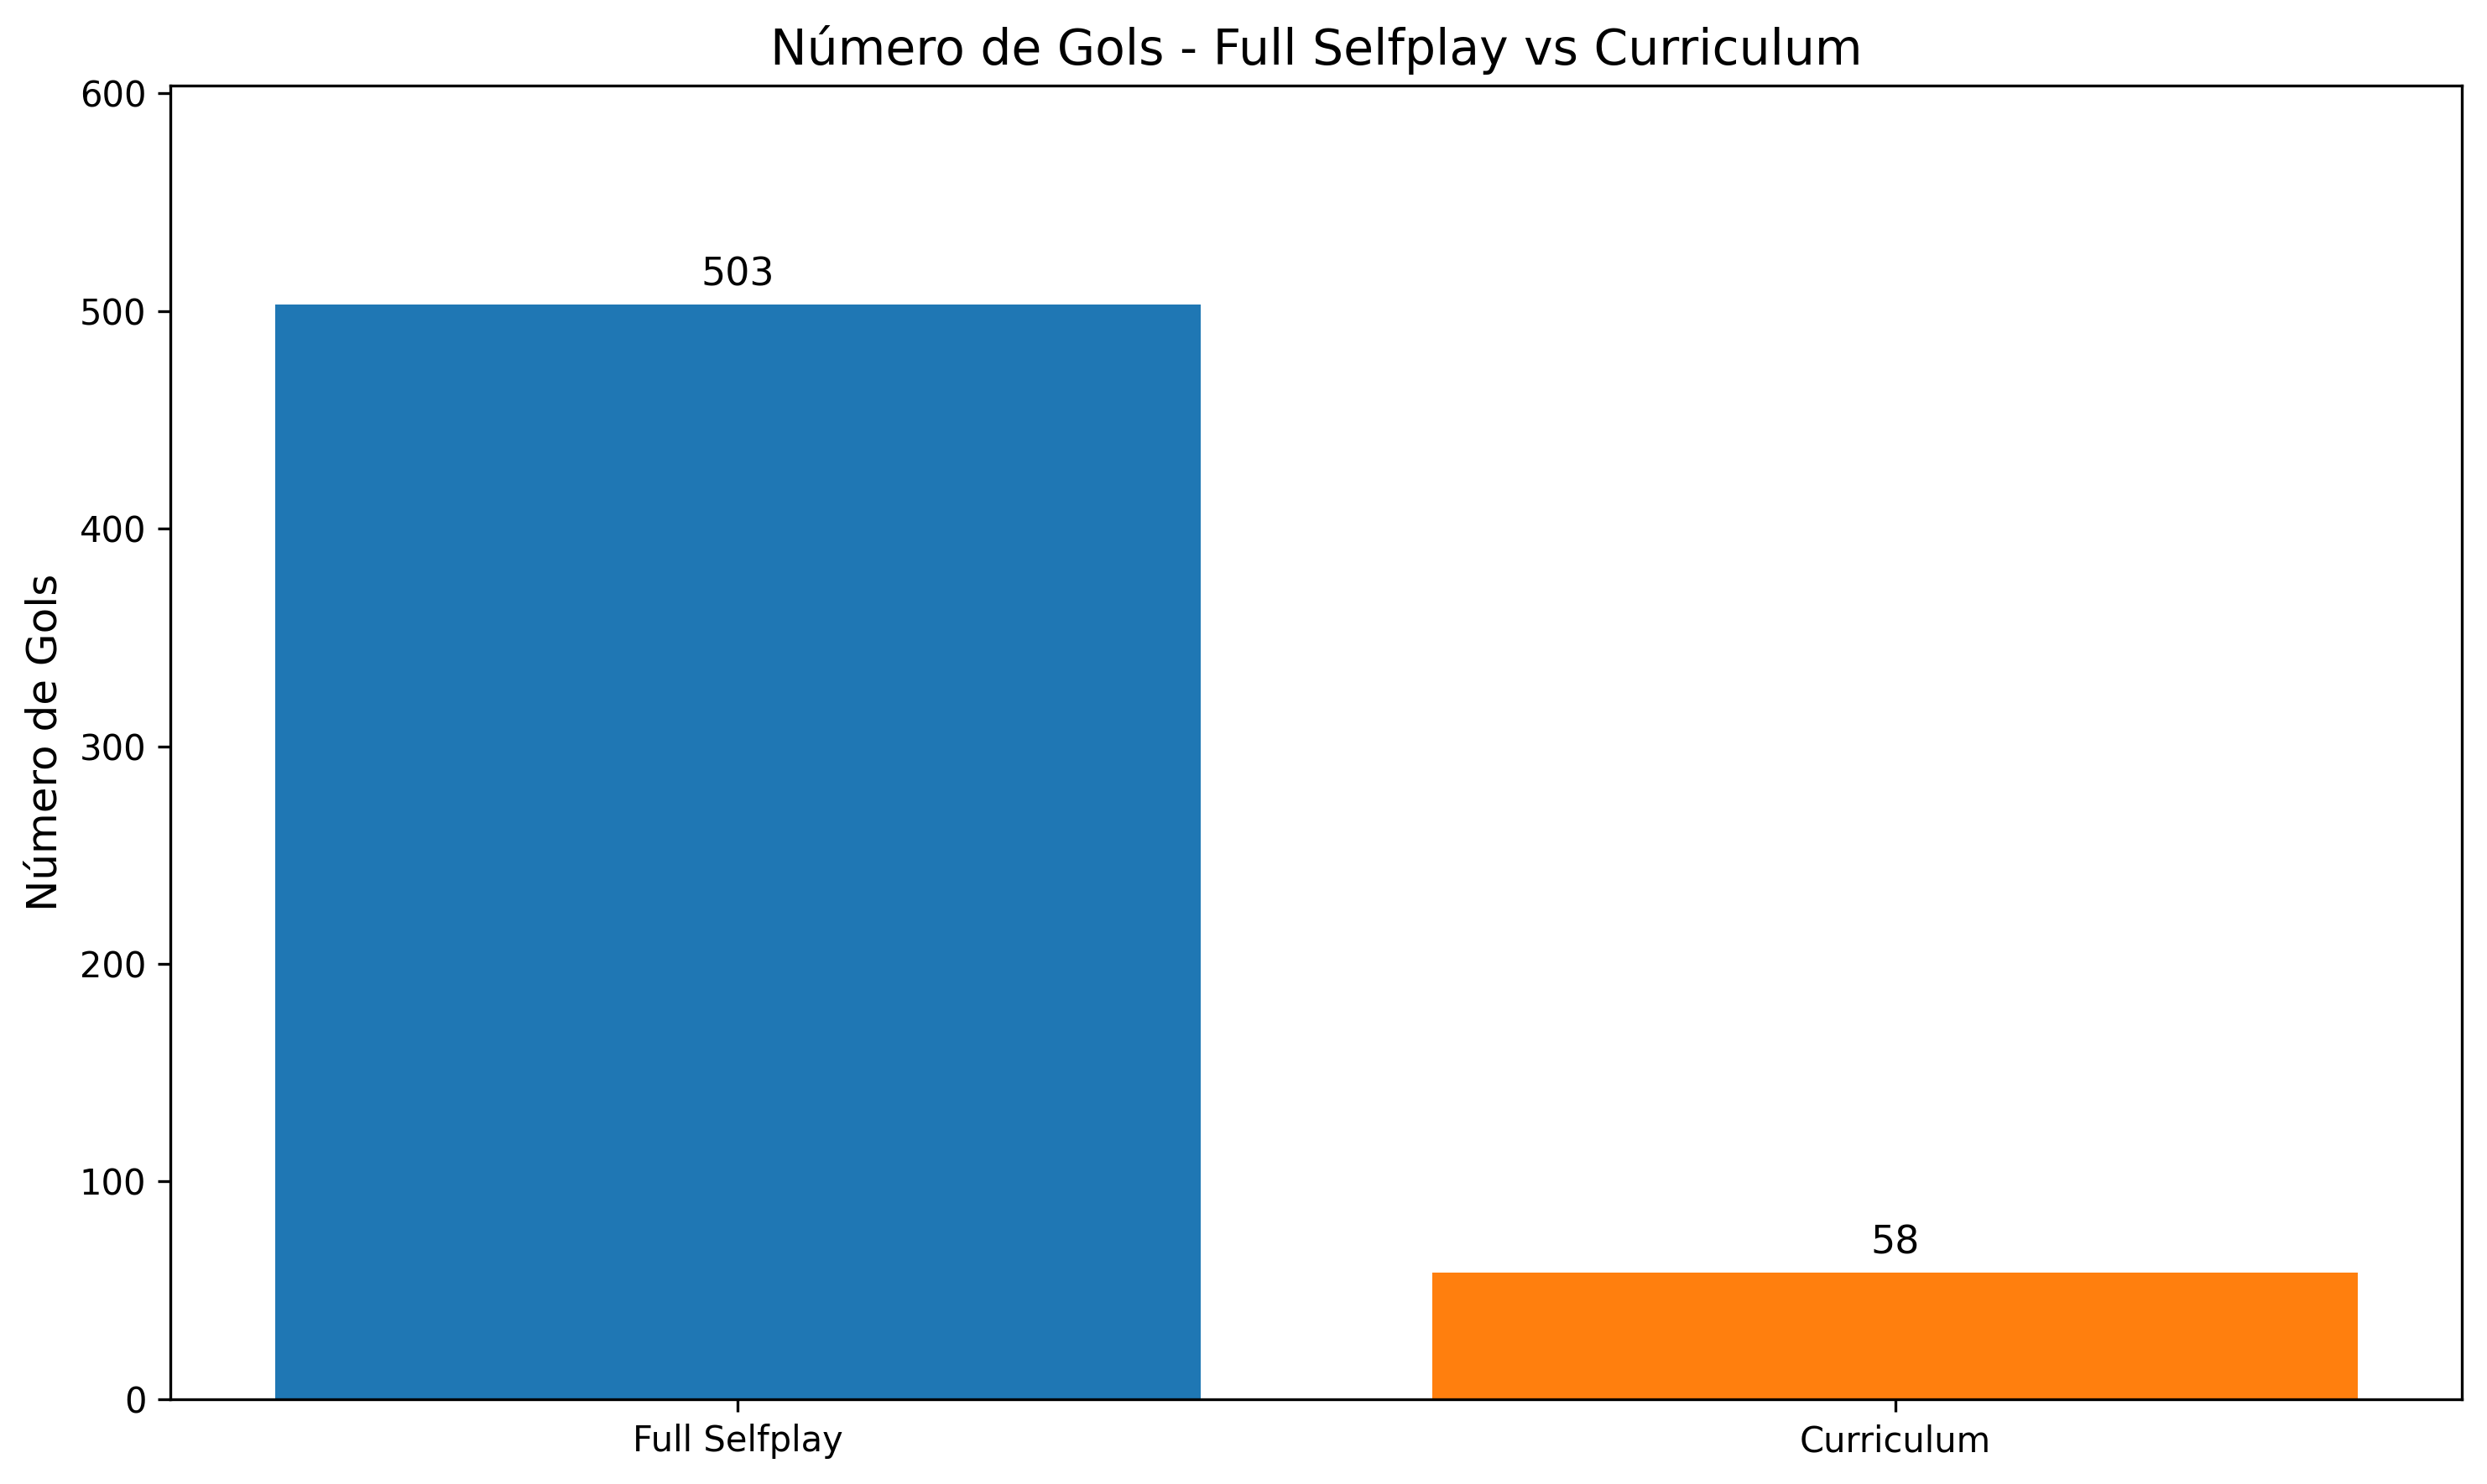
\includegraphics[width=0.8\textwidth]{fig/graficos_trabalho/graficos_torneios/torneios/gols_full_selfplay_vs_curriculum.png}
    \caption{Comparação de gols marcados no Torneio 1: \textit{Full Selfplay} vs \textit{Curriculum}}
    \label{fig:gols_torneio1}
\end{figure}

\begin{figure}[H]
    \centering
    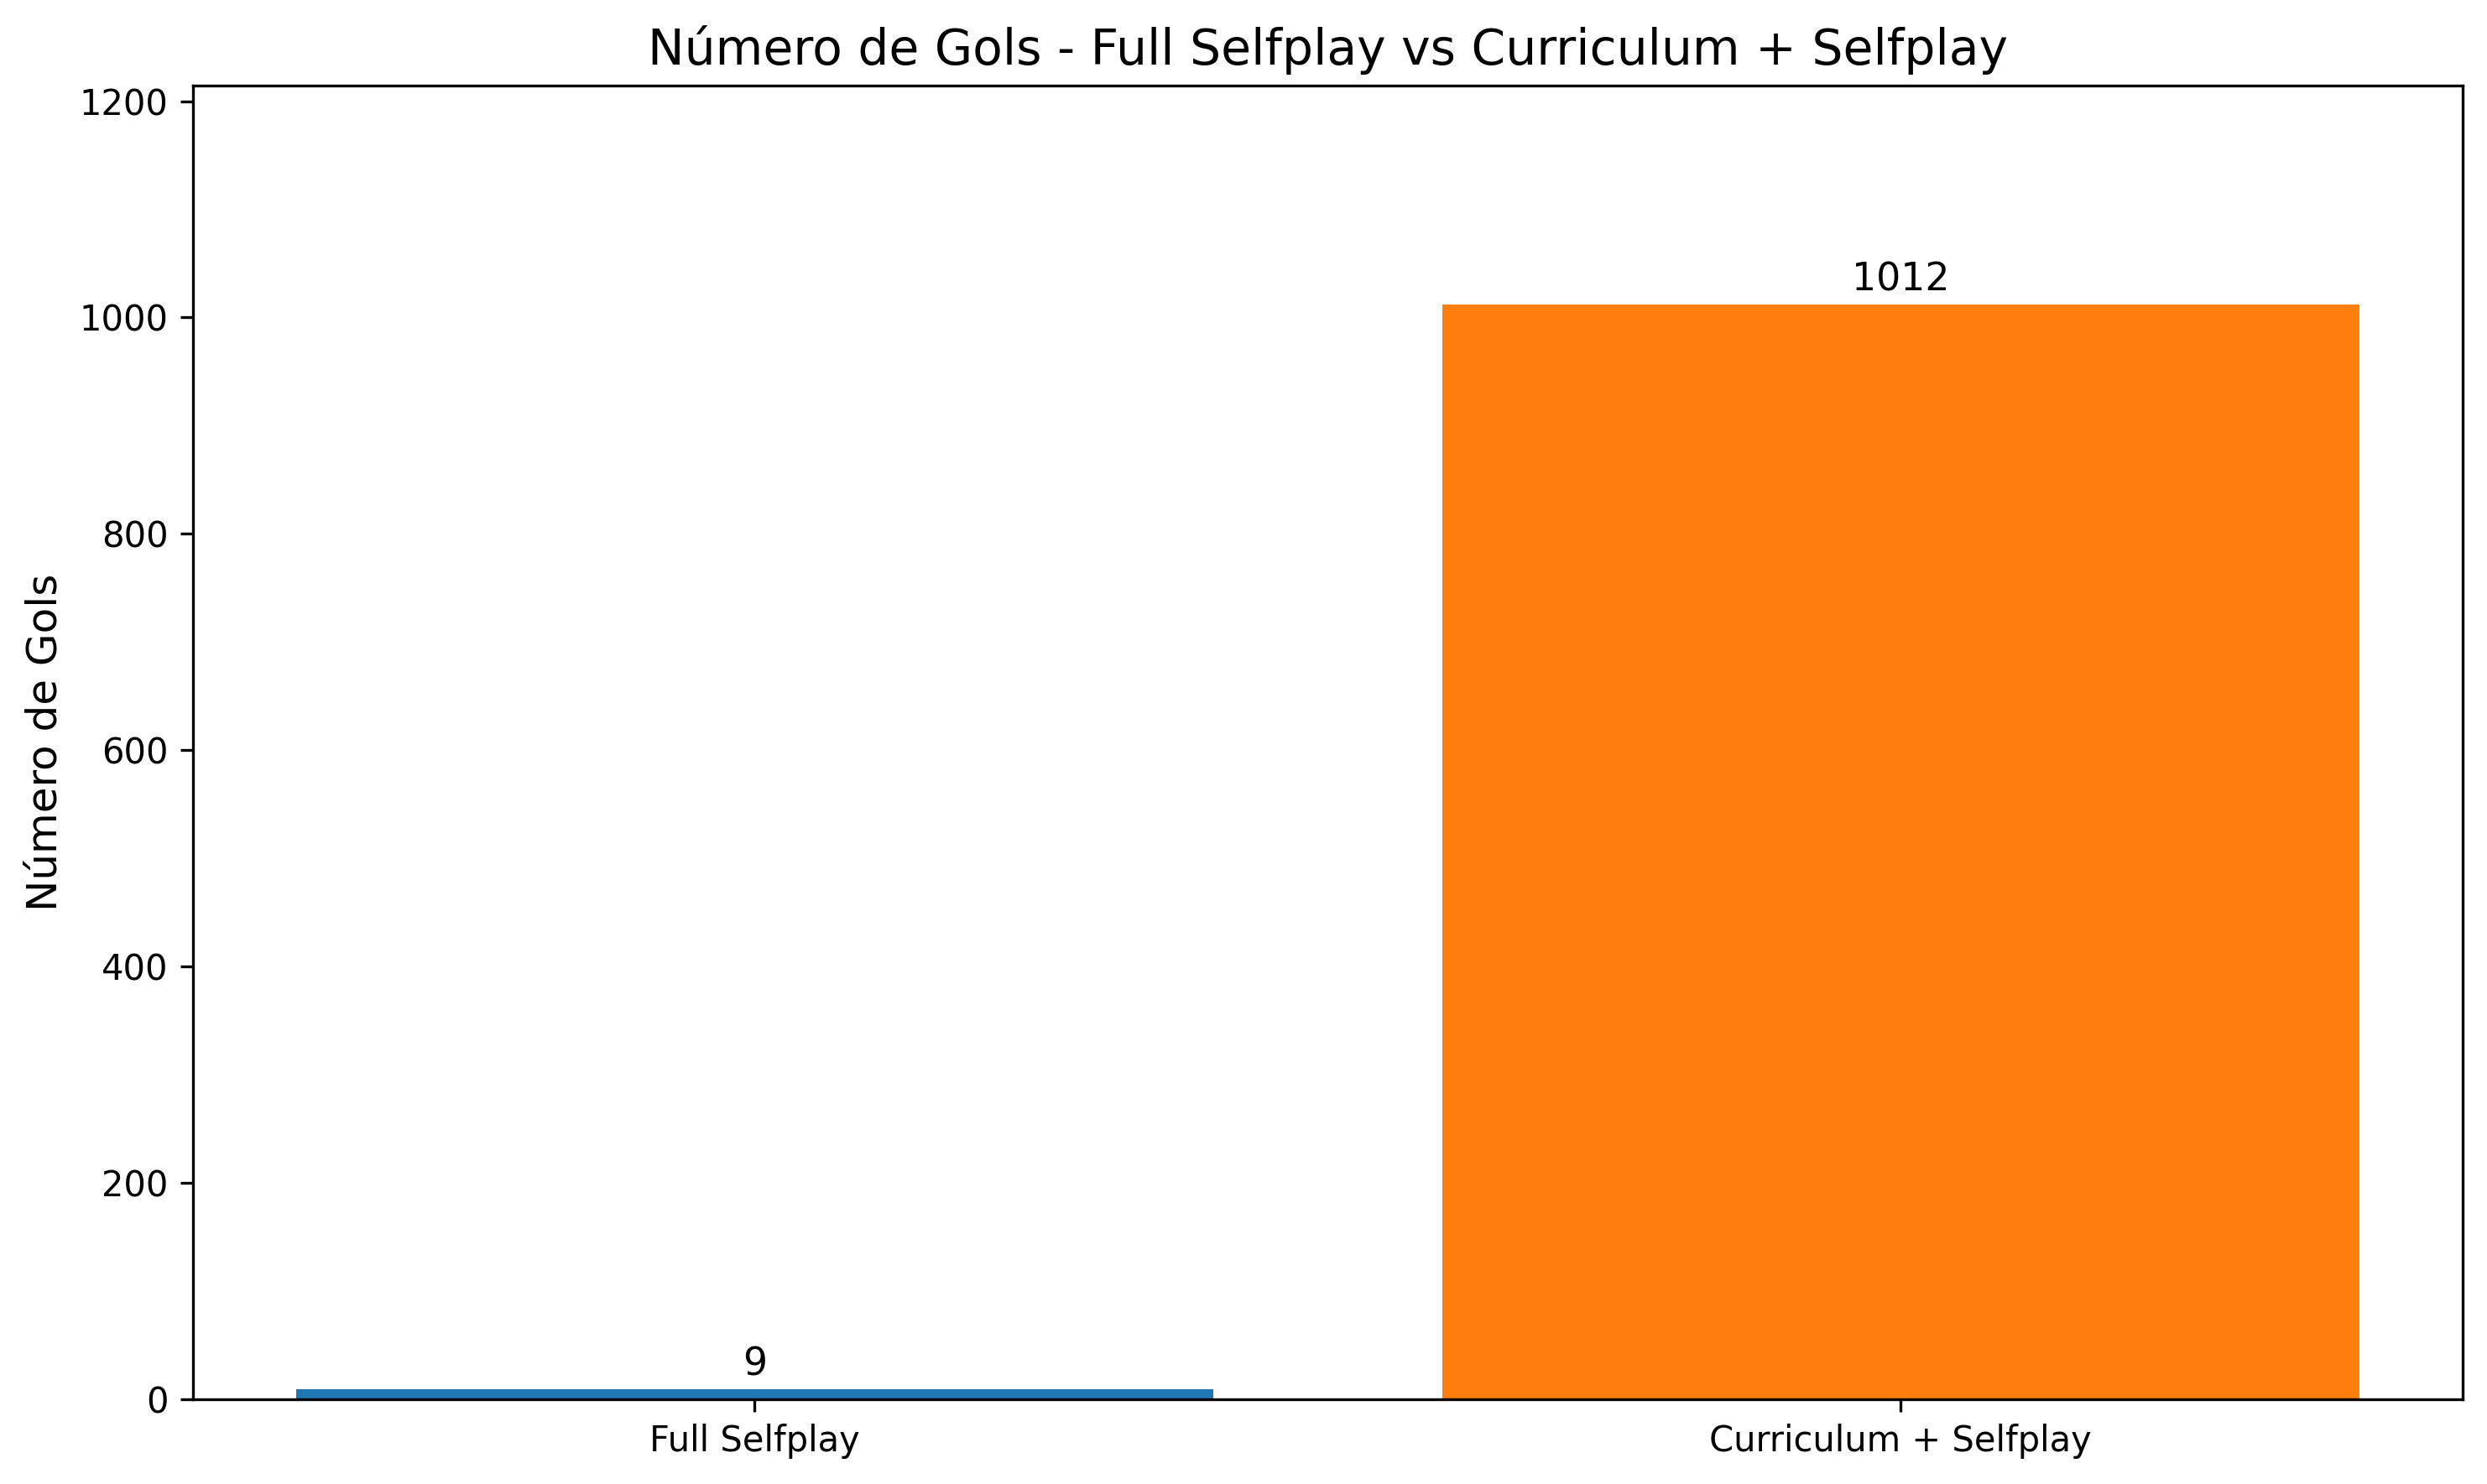
\includegraphics[width=0.8\textwidth]{fig/graficos_trabalho/graficos_torneios/torneios/gols_full_selfplay_vs_curriculum_+_selfplay.png}
    \caption{Comparação de gols marcados no Torneio 2: \textit{Full Selfplay} vs \textit{Curriculum} + \textit{Selfplay}}
    \label{fig:gols_torneio2}
\end{figure}

A análise dos gols marcados em cada torneio revela padrões consistentes com os resultados gerais das partidas, mas com diferenças de magnitude ainda mais pronunciadas.

No Torneio 1 (\textit{Full Selfplay} vs \textit{Curriculum}), o modelo treinado apenas com \textit{self-play} demonstrou capacidade ofensiva significativamente superior, marcando 503 gols durante as 500 partidas, o que corresponde a uma média de 1,006 gols por partida. Em contraste, o modelo treinado exclusivamente com \textit{curriculum learning} marcou apenas 58 gols (média de 0,116 por partida), aproximadamente 11,5\% do desempenho ofensivo do \textit{Full Selfplay}.

Esta disparidade sugere que, embora o \textit{curriculum learning} desenvolva habilidades fundamentais, ele não é suficiente para criar agentes com capacidade ofensiva efetiva em um cenário competitivo completo. A limitação ofensiva explica o alto número de empates e a baixa taxa de vitórias do modelo \textit{Curriculum}.

No Torneio 2 (\textit{Full Selfplay} vs \textit{Curriculum} + \textit{Selfplay}), observamos uma inversão dramática deste padrão. O modelo combinado (\textit{curriculum} + \textit{self-play}) apresentou uma capacidade ofensiva diferenciada, marcando 1.012 gols durante as 500 partidas, o que corresponde a uma impressionante média de 2,024 gols por partida. Em contraste, o modelo \textit{Full Selfplay} marcou apenas 9 gols (média de 0,018 por partida), menos de 1\% do desempenho ofensivo do modelo combinado (9 gols em 500 partidas).

Esta grande disparidade na capacidade ofensiva pode ser atribuída ao resultado sinérgico da abordagem combinada. O \textit{curriculum learning} proporciona uma base sólida de habilidades fundamentais que, quando refinadas através do \textit{self-play}, resultam em estratégias ofensivas excepcionalmente eficazes. O contraste entre o desempenho do \textit{Full Selfplay} nos dois torneios sugere que o modelo combinado não apenas desenvolve políticas superiores, mas também consegue neutralizar efetivamente as estratégias do \textit{Full Selfplay}, limitando drasticamente sua capacidade ofensiva.

\subsection{Análise de Trade-offs entre Abordagens}

Uma observação importante que surge da análise dos dados dos torneios é o claro \textit{trade-off} entre as diferentes abordagens de treinamento. A Tabela \ref{tab:comparacao_abordagens_detalhada} resume as principais métricas para cada abordagem nos confrontos diretos, facilitando a visualização destes \textit{trade-offs}.

\begin{table}[H]
    \centering
    \begin{tabular}{|c|c|c|}
        \hline
        \textbf{Métrica} & \textbf{Curriculum} & \textbf{Curriculum + Self-play} \\
        \hline
        Vitórias vs Full Self-play & 33 (6,6\%) & 430 (86\%) \\
        \hline
        Empates vs Full Self-play & 220 (44\%) & 63 (12,6\%) \\
        \hline
        Derrotas vs Full Self-play & 247 (49,4\%) & 7 (1,4\%) \\
        \hline
        Gols marcados vs Full Self-play & 58 & 1.012 \\
        \hline
        Gols sofridos vs Full Self-play & 503 & 9 \\
        \hline
        Média de gols/partida & 0,116 & 2,024 \\
        \hline
    \end{tabular}
    \caption{Comparação detalhada entre as abordagens de treinamento nos torneios}
    \label{tab:comparacao_abordagens_detalhada}
\end{table}

A análise desta tabela revela padrões claros que caracterizam cada abordagem:

\begin{enumerate}
    \item \textbf{Curriculum Learning puro}: Desenvolve agentes com capacidades defensivas significativas, evidenciadas pelo alto número de empates (44\%) mesmo contra o \textit{Full Self-play}. No entanto, apresenta limitações severas na capacidade ofensiva, com apenas 0,116 gols por partida e baixa taxa de vitórias (6,6\%). Sua estratégia parece focada na neutralização do adversário, mas com dificuldades para criar situações ofensivas efetivas.
    
    \item \textbf{Full Self-play}: Produz agentes com capacidades ofensivas e defensivas moderadamente equilibradas, conseguindo dominar o \textit{Curriculum} puro (49,4\% de vitórias), mas sendo completamente superado pela abordagem combinada (apenas 1,4\% de vitórias). Esta abordagem baseia-se na exploração auto-dirigida do espaço de estados, resultando em políticas funcionais, mas subótimas.
    
    \item \textbf{Curriculum + Self-play}: Representa uma síntese poderosa que maximiza os benefícios de ambas as abordagens anteriores. Demonstra capacidade ofensiva extraordinária (2,024 gols por partida) combinada com defesa quase impenetrável (apenas 9 gols sofridos em 500 partidas). O resultado é uma dominância esmagadora sobre o \textit{Full Self-play}, com 86\% de vitórias e mais de 100 vezes mais gols marcados.
\end{enumerate}

Estes resultados confirmam a hipótese central deste trabalho: o \textit{curriculum learning} proporciona fundamentos sólidos que, quando refinados através do \textit{self-play} competitivo, resultam em políticas significativamente superiores às desenvolvidas por qualquer uma das abordagens isoladamente.

A análise dos torneios revela aspectos particularmente interessantes sobre a transferência de conhecimento entre fases de treinamento. O modelo \textit{Curriculum} puro, embora limitado ofensivamente, demonstra capacidades defensivas substanciais, como evidenciado pelo alto número de empates contra o \textit{Full Self-play}. Quando estas capacidades defensivas são combinadas com o refinamento tático proporcionado pelo \textit{self-play}, o resultado é um agente com defesa sólida e ataque extremamente eficaz.

Um aspecto notável é a diferença no desempenho do \textit{Full Self-play} entre os dois torneios. Contra o \textit{Curriculum} puro, ele demonstra dominância clara, mas contra o \textit{Curriculum} + \textit{Self-play}, seu desempenho colapsa. Isto sugere que a abordagem combinada não apenas desenvolve políticas eficazes, mas também consegue neutralizar estrategicamente as políticas aprendidas pelo \textit{Full Self-play}, explorando suas vulnerabilidades de forma sistemática.

Em síntese, a abordagem combinada \textit{Curriculum} + \textit{Self-play} demonstra o melhor equilíbrio entre capacidades ofensivas e defensivas, com uma superioridade que transcende a simples soma das vantagens individuais de cada método. Este efeito sinérgico valida a importância do desenvolvimento estruturado de habilidades fundamentais antes da exposição a cenários competitivos complexos, estabelecendo um paradigma promissor para o treinamento de agentes em ambientes multiagente como o futebol de robôs.


Para complementar a análise quantitativa apresentada, foram registradas gravações ilustrativas de algumas partidas dos torneios realizados. Estas gravações servem como demonstração visual das diferentes estratégias e comportamentos emergentes discutidos anteriormente, e podem ser encontradas online\footnote{\url{https://drive.google.com/drive/folders/1dT-Bp7ocl20wf2JIIIZPvPQepCzyFvfx?usp=sharing}}.







\section{Análise das Métricas de Aprendizado por Reforço}
\label{sec:analise_metricas_aprendizado}

Além das métricas específicas do domínio do futebol de robôs, uma análise detalhada das métricas básicas de aprendizado por reforço fornece \textit{insights} valiosos sobre os processos internos dos algoritmos durante o treinamento. Esta seção explora três métricas fundamentais: entropia da política, perda da política e variância explicada da função valor, comparando o comportamento dessas métricas entre as abordagens \textit{Selfplay} após \textit{Curriculum} e \textit{Full Selfplay}.

\subsection{Entropia da Política}

A entropia da política é uma métrica que quantifica o grau de aleatoriedade ou exploração nas decisões do agente. Valores mais altos (menos negativos) indicam maior exploração, enquanto valores mais baixos (mais negativos) sugerem maior certeza nas ações escolhidas. A Figura \ref{fig:policy_entropy} apresenta a comparação da entropia da política entre as duas abordagens ao longo do treinamento.

\begin{figure}[H]
    \centering
    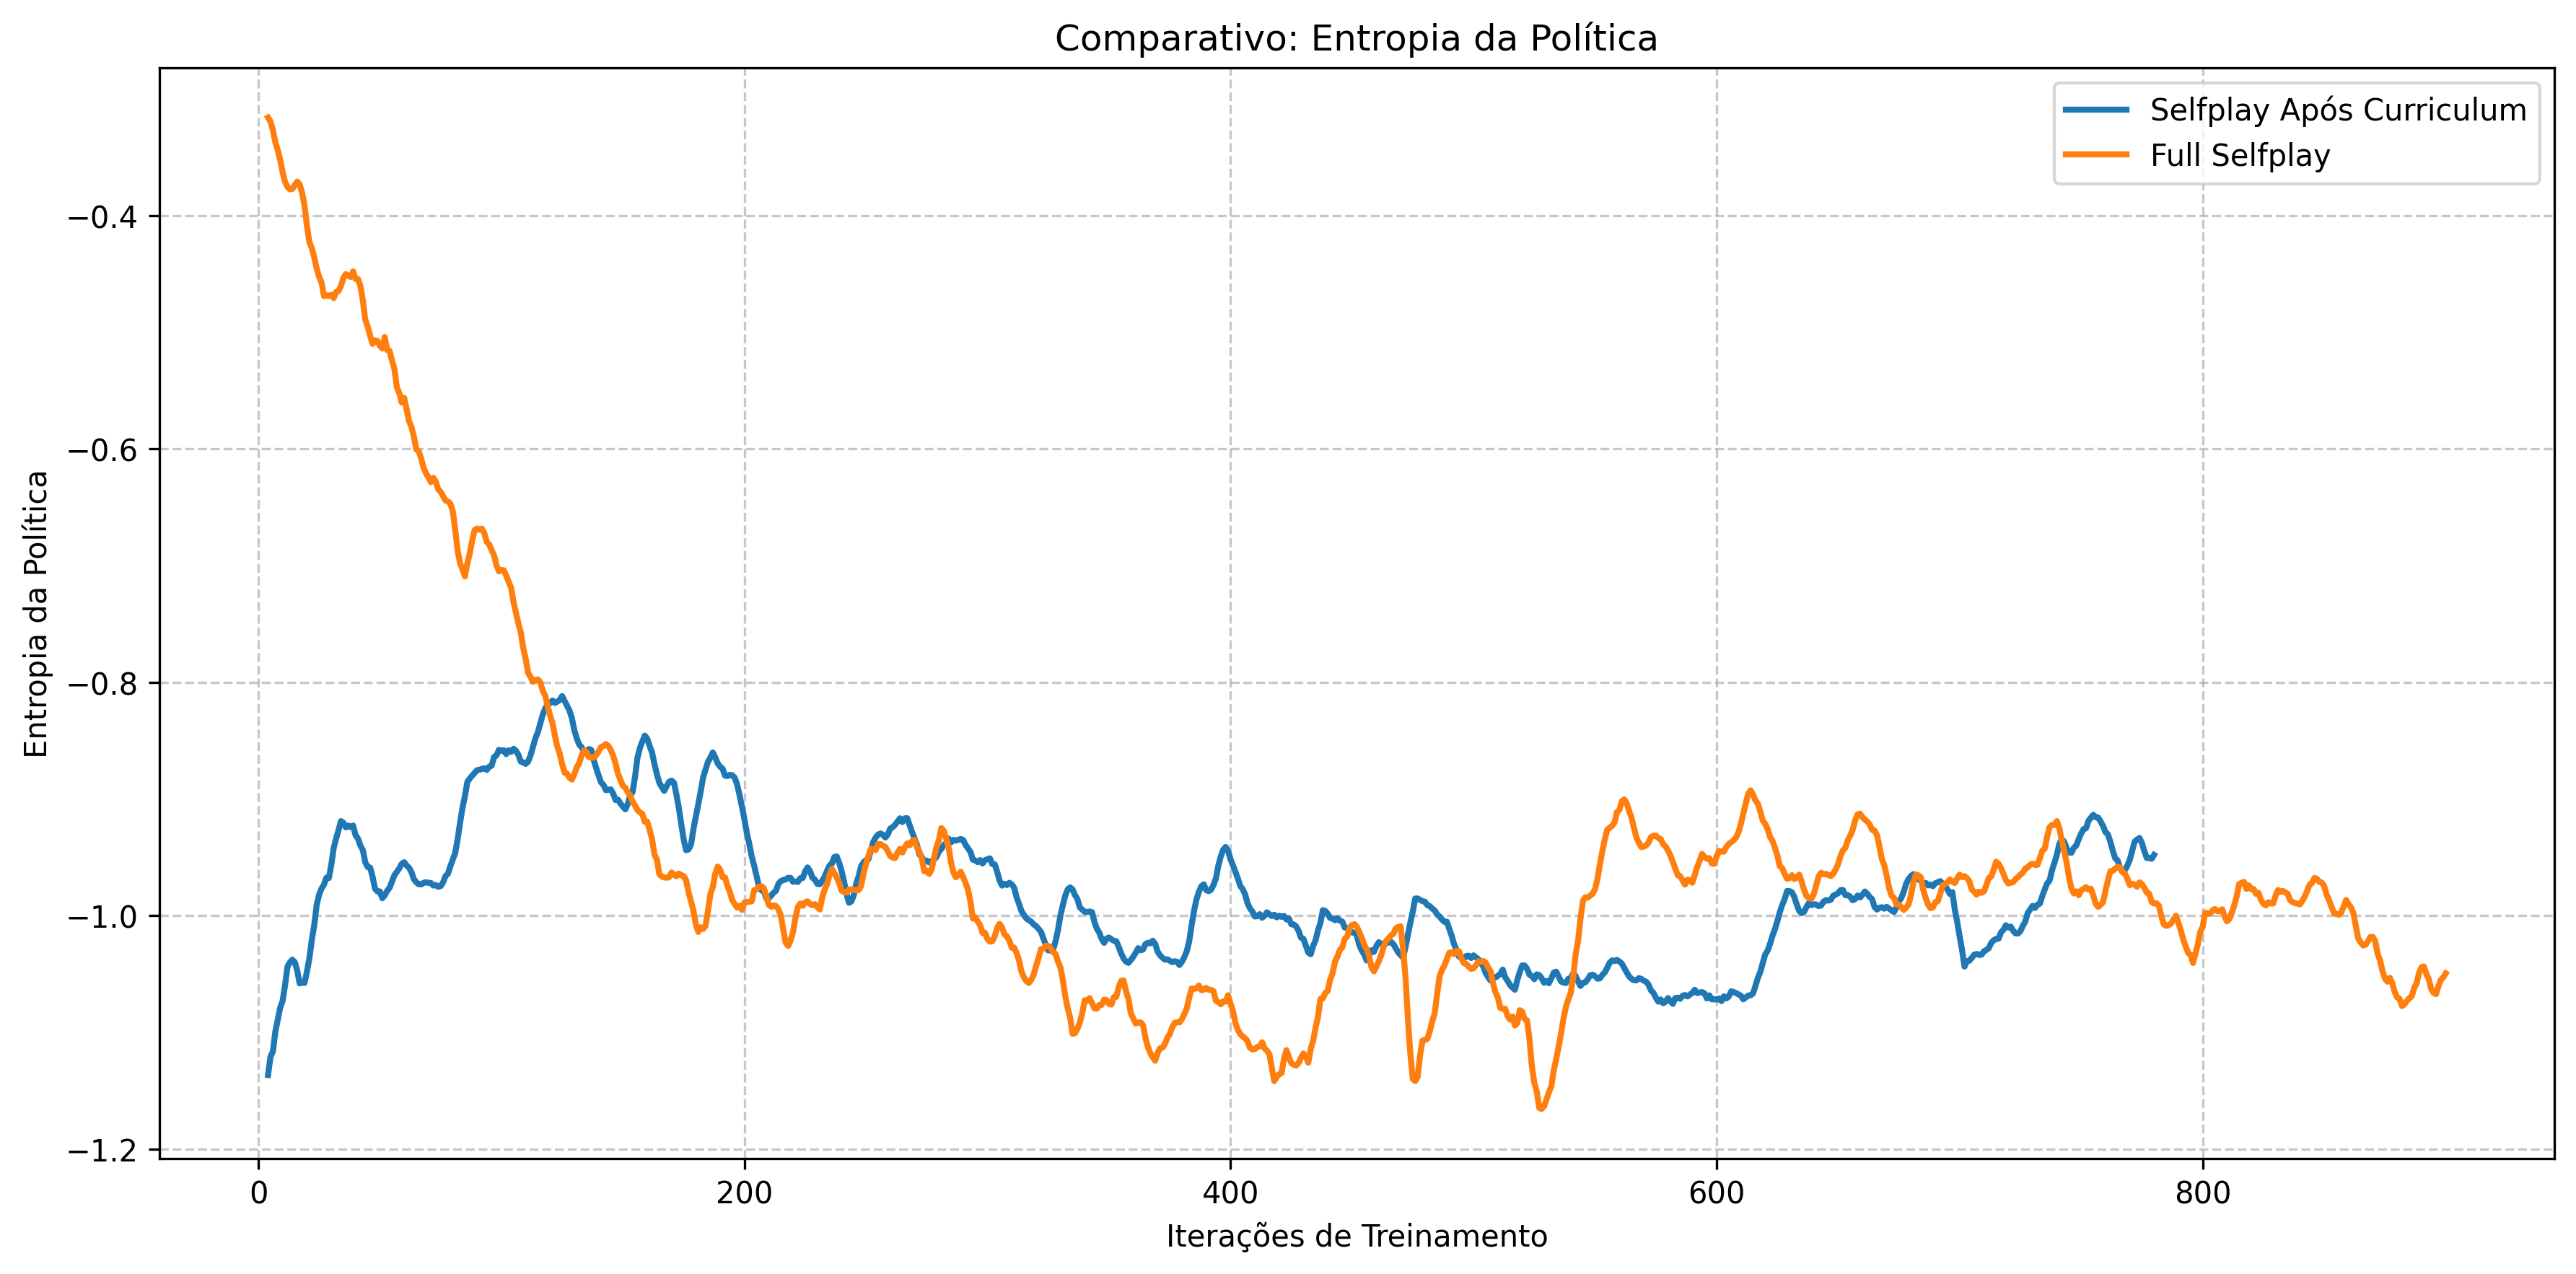
\includegraphics[width=0.95\textwidth]{fig/graficos_trabalho/graficos_experimentos/geral/comparativo_entropia_politica.png}
    \caption{Comparativo da entropia da política: \textit{Selfplay} após \textit{Curriculum} e \textit{Full Selfplay}}
    \label{fig:policy_entropy}
\end{figure}

A análise do gráfico revela diferenças significativas nos padrões de exploração-explotação entre as duas abordagens. O \textit{Full Selfplay} (linha laranja) inicia o treinamento com valores de entropia mais altos (próximos a -0,3), indicando uma política mais exploratória, o que é esperado para agentes que começam o aprendizado sem conhecimento prévio. Em contraste, o \textit{Selfplay} após \textit{Curriculum} (linha azul) começa com valores de entropia significativamente mais baixos (aproximadamente -1,1), sugerindo uma política já mais determinística.

Esta diferença inicial é particularmente reveladora: agentes treinados com \textit{curriculum learning} iniciam a fase de \textit{selfplay} com políticas mais refinadas e menos aleatórias, evidenciando que o conhecimento adquirido durante os estágios do \textit{curriculum} proporciona maior certeza nas ações a serem tomadas.

Após aproximadamente 150-200 iterações, observa-se uma convergência nas entropias, com ambas as abordagens chegando a valores similares. No entanto, é notável que o \textit{Full Selfplay} apresenta maior volatilidade ao longo de todo o treinamento, com oscilações mais pronunciadas, enquanto o \textit{Selfplay} após \textit{Curriculum} mantém níveis mais estáveis de entropia, sugerindo um processo de aprendizado mais consistente e menos errático.

\subsection{Perda da Política}

A perda da política é uma métrica que reflete a divergência entre a política atual e a política que seria ótima segundo as estimativas atuais da função de valor. Em algoritmos como \textit{PPO}, a minimização desta perda é um dos objetivos principais do processo de otimização. A Figura \ref{fig:policy_loss} apresenta a evolução desta métrica durante o treinamento.

\begin{figure}[H]
    \centering
    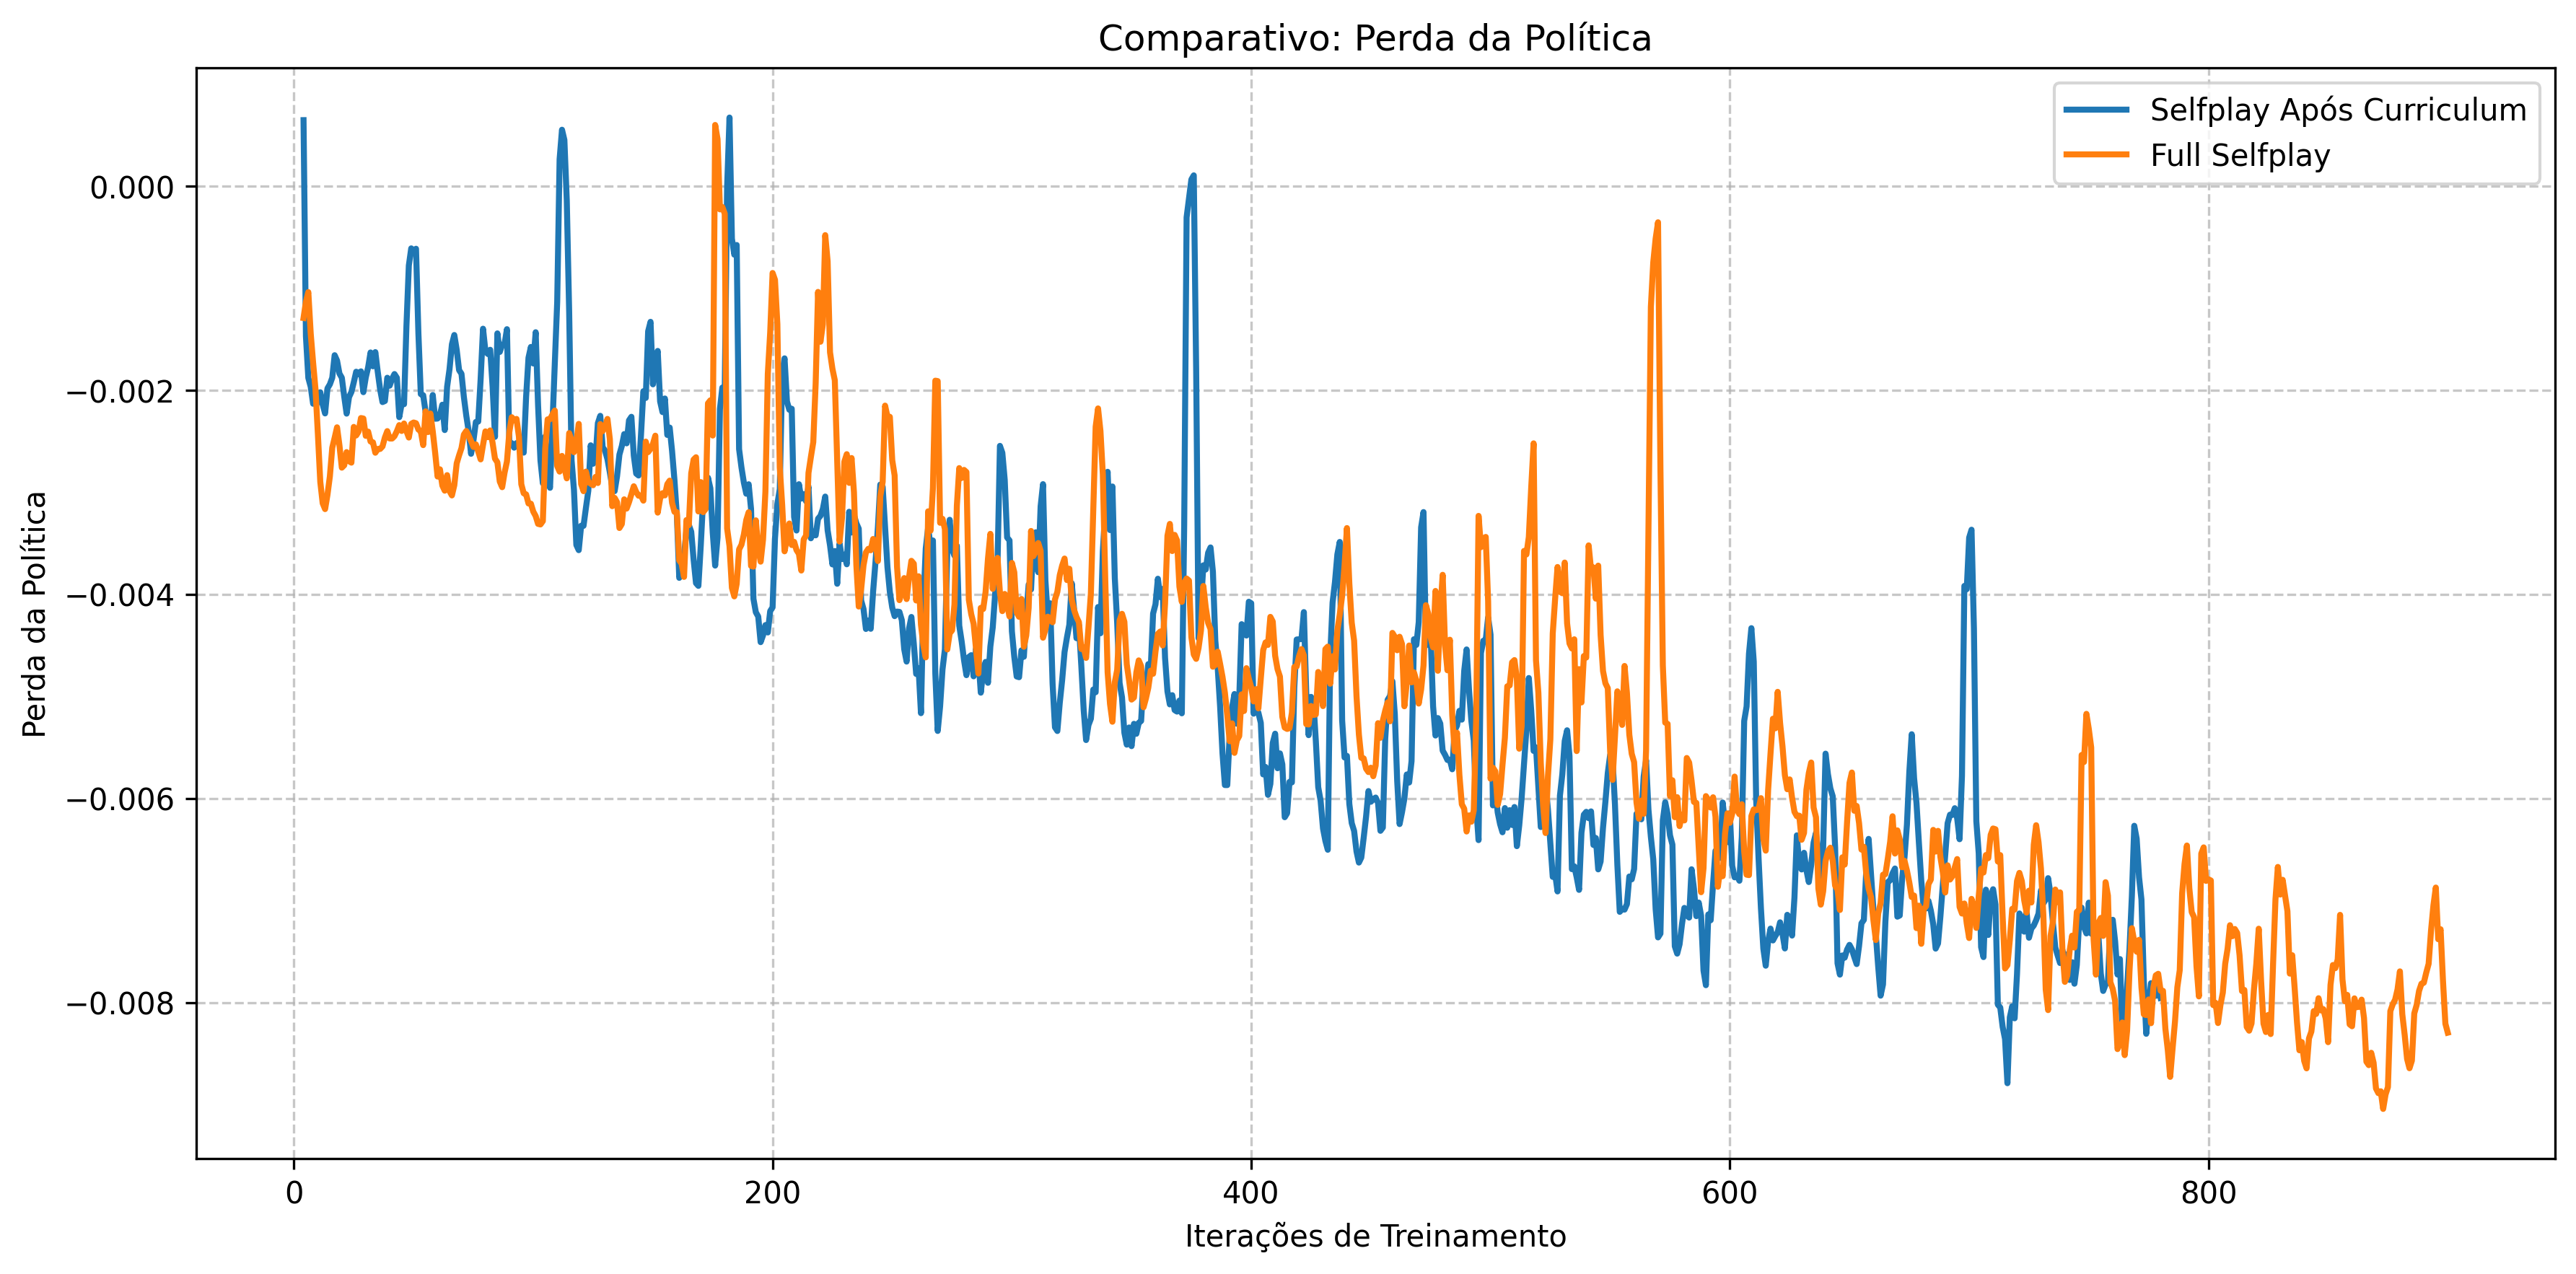
\includegraphics[width=0.95\textwidth]{fig/graficos_trabalho/graficos_experimentos/geral/comparativo_perda_politica.png}
    \caption{Comparativo da perda da política: \textit{Selfplay} após \textit{Curriculum} e \textit{Full Selfplay}}
    \label{fig:policy_loss}
\end{figure}

O gráfico de perda da política mostra um comportamento interessante: ambas as abordagens iniciam com valores similares e seguem uma tendência geral de redução da perda ao longo do treinamento, o que indica uma melhoria progressiva nas políticas. No entanto, há diferenças notáveis na trajetória dessa redução.

Observa-se que ambas as abordagens apresentam alta volatilidade, com várias oscilações ao longo do processo. Esta característica é típica de ambientes competitivos como o \textit{self-play}, onde as mudanças na política de um oponente podem temporariamente aumentar a perda até que o agente se adapte.

Um aspecto particularmente relevante é que o \textit{Full Selfplay} continua seu treinamento por mais iterações e alcança valores de perda mais negativos nas fases finais. Isto pode indicar que, sem o benefício do \textit{curriculum} inicial, esta abordagem requer um período mais longo de refinamento para atingir níveis comparáveis de otimização da política.

A análise conjunta com as outras métricas sugere que, embora o \textit{Full Selfplay} eventualmente alcance valores de perda similares ou até melhores, o caminho para chegar a este ponto é mais longo e menos eficiente comparado ao \textit{Selfplay} após \textit{Curriculum}.

\subsection{Variância Explicada da Função Valor}

A variância explicada é uma métrica que avalia a qualidade da função valor aprendida pelo agente, indicando quão bem o modelo consegue prever retornos futuros. Valores próximos a 1 indicam alta precisão nas previsões, enquanto valores mais baixos sugerem maior incerteza. A Figura \ref{fig:explained_variance} apresenta a comparação desta métrica entre as duas abordagens.

\begin{figure}[H]
    \centering
    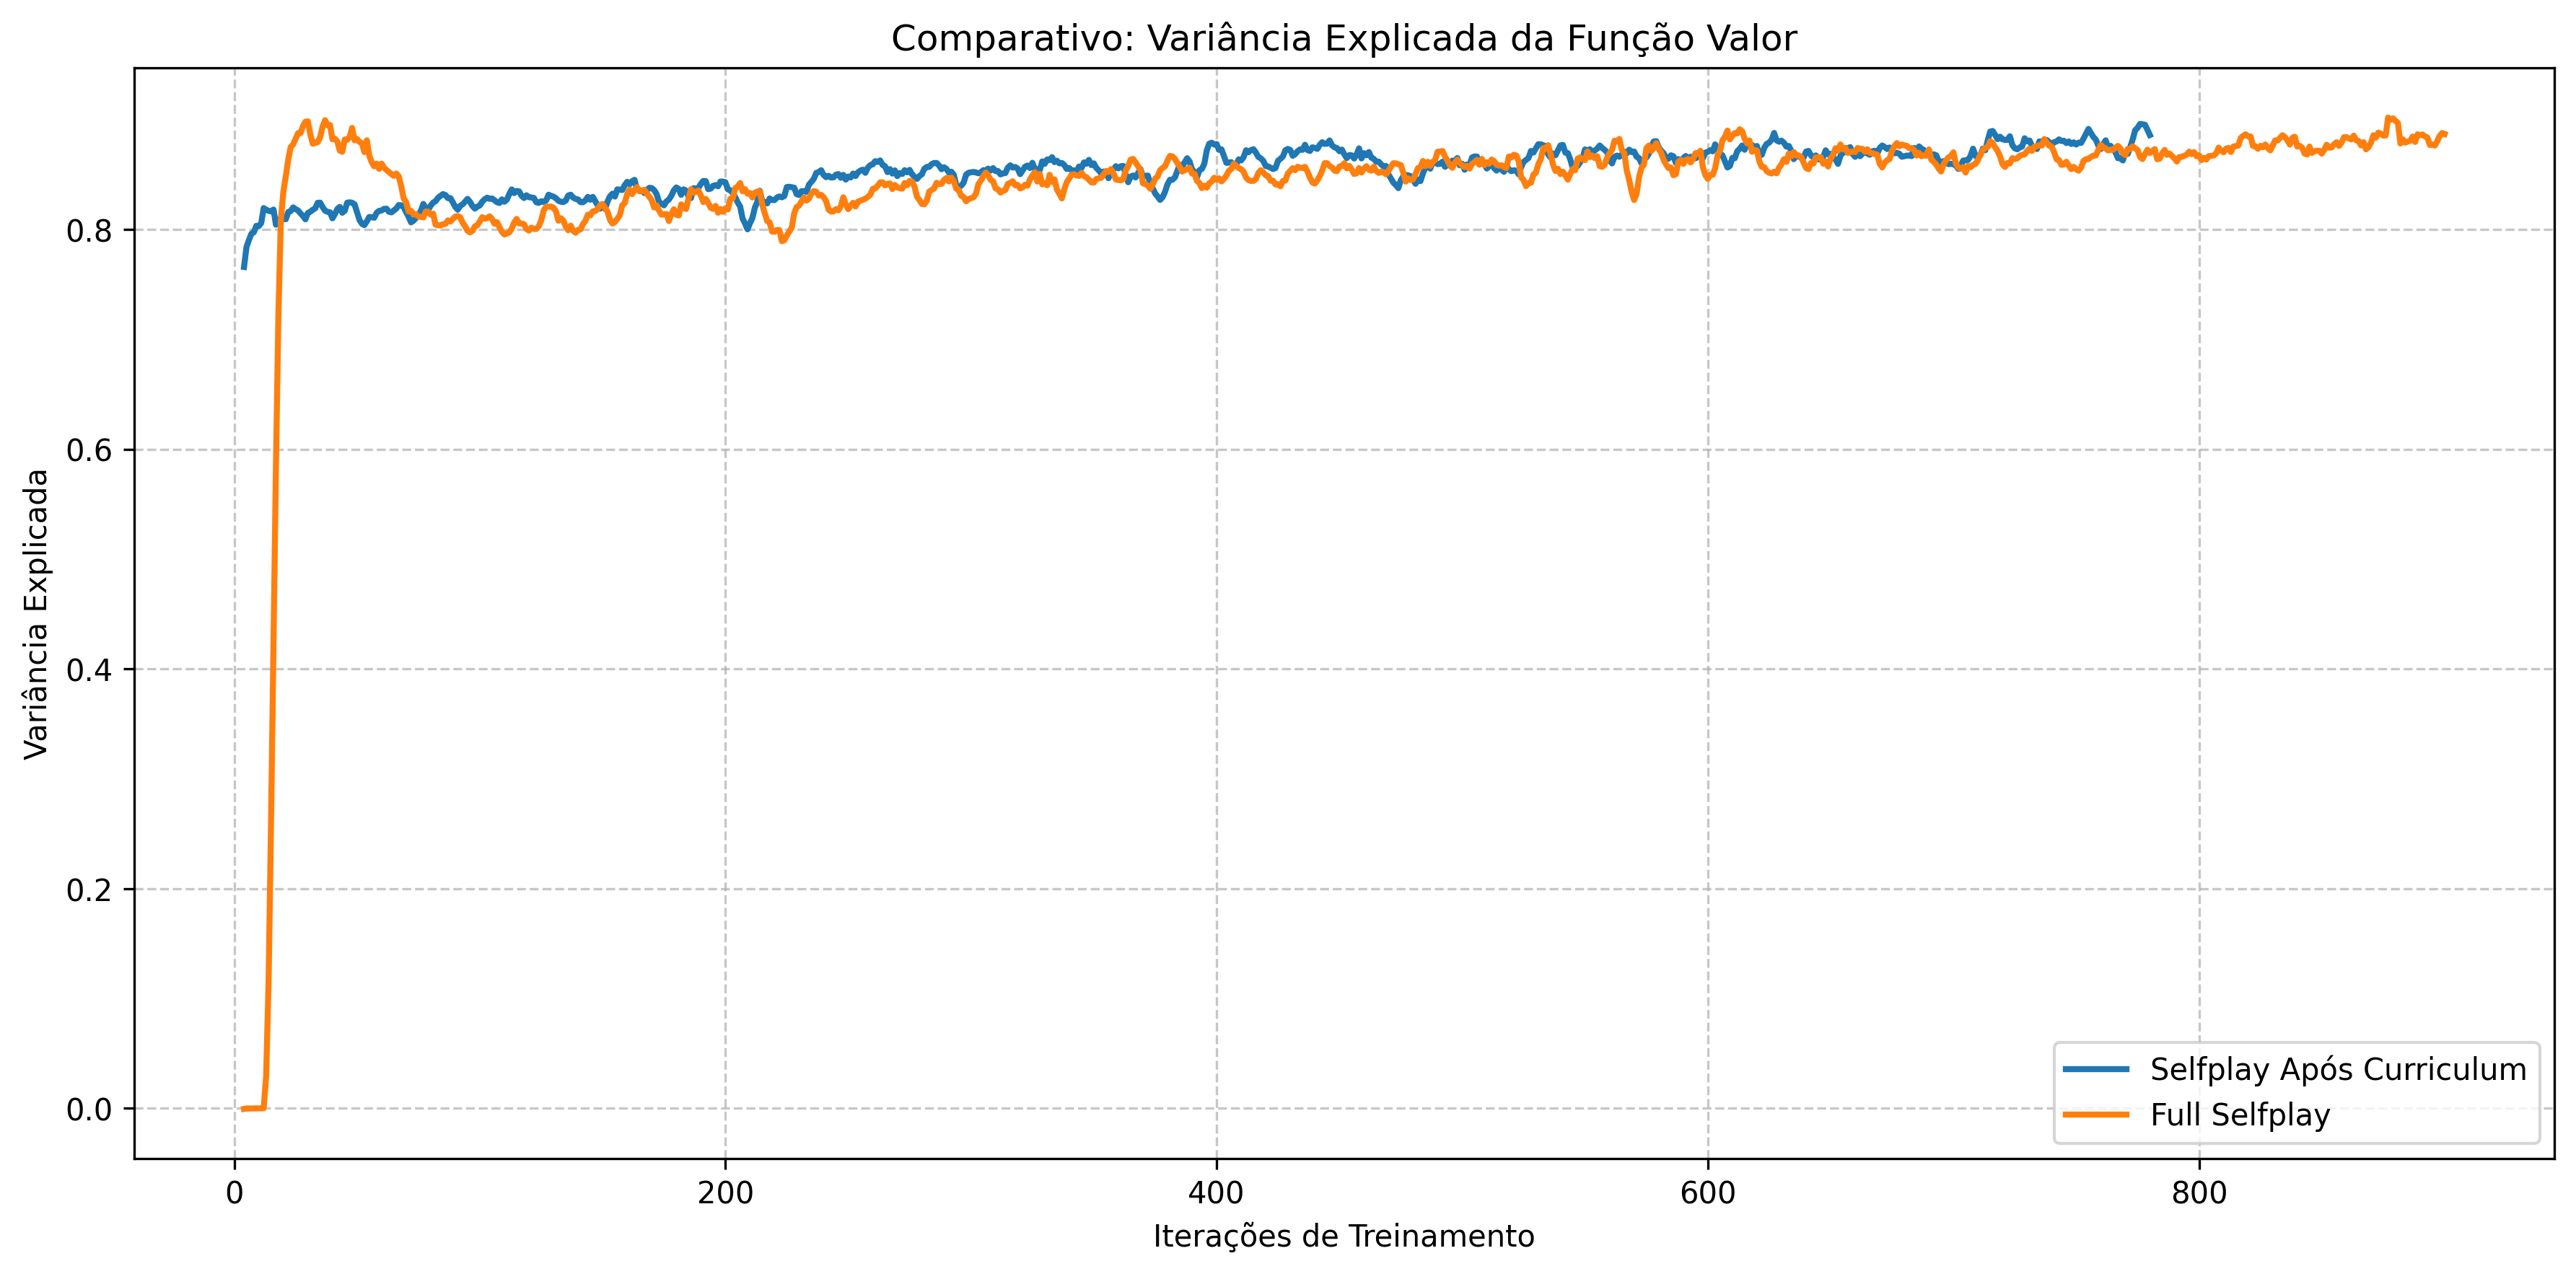
\includegraphics[width=0.95\textwidth]{fig/graficos_trabalho/graficos_experimentos/geral/comparativo_variancia_explicada.png}
    \caption{Comparativo da variância explicada da função valor: \textit{Selfplay} após \textit{Curriculum} e \textit{Full Selfplay}}
    \label{fig:explained_variance}
\end{figure}

A análise do gráfico de variância explicada revela padrões distintos no desenvolvimento da função valor. O \textit{Full Selfplay} (linha laranja) apresenta um comportamento curioso nas primeiras iterações, com um pico inicial seguido por uma queda abrupta. Este padrão pode ser atribuído a uma superestimação inicial da capacidade preditiva, seguida por um ajuste à medida que o agente enfrenta situações mais diversificadas.

Em contraste, o \textit{Selfplay} após \textit{Curriculum} (linha azul) inicia com valores mais estáveis, sem os extremos observados no \textit{Full Selfplay}. Esta estabilidade inicial é mais uma evidência dos benefícios do treinamento curricular prévio, que proporciona ao agente uma base mais sólida para estimar recompensas futuras.

Após aproximadamente 200 iterações, ambas as abordagens convergem para valores similares de variância explicada, em torno de 0,85, indicando que ambos os métodos eventualmente desenvolvem funções valor de qualidade comparável. No entanto, o caminho para atingir esta convergência é notavelmente diferente, com o \textit{Selfplay} após \textit{Curriculum} demonstrando maior consistência ao longo do processo.

Nas fases finais do treinamento, após a convergência, ambas as abordagens mantêm níveis similares e estáveis de variância explicada, sugerindo que, embora o processo de aprendizado seja diferente, o resultado final em termos de capacidade preditiva da função valor é comparável.

\subsection{Implicações para o Processo de Aprendizagem}

A análise integrada das três métricas básicas de aprendizado por reforço revela padrões consistentes que destacam as diferenças fundamentais entre as abordagens \textit{Selfplay} após \textit{Curriculum} e \textit{Full Selfplay}.

Em primeiro lugar, observa-se que o \textit{Selfplay} após \textit{Curriculum} consistentemente demonstra maior estabilidade nas fases iniciais e intermediárias do treinamento. Esta característica é particularmente valiosa em cenários complexos como o futebol de robôs, onde a volatilidade excessiva pode levar a políticas subótimas ou comportamentos indesejados.

Em segundo lugar, a transição mais suave nas métricas de aprendizado do \textit{Selfplay} após \textit{Curriculum} sugere que o conhecimento adquirido durante os estágios do \textit{curriculum} proporciona um ponto de partida mais avançado para o desenvolvimento de políticas competitivas. Esta vantagem inicial se traduz em um processo de aprendizado mais eficiente, requerendo menos iterações para atingir níveis comparáveis de desempenho.

Por fim, embora ambas as abordagens eventualmente convirjam para valores similares nas métricas analisadas, o caminho para esta convergência é significativamente diferente. O \textit{Selfplay} após \textit{Curriculum} oferece um processo de aprendizado mais direto e consistente, enquanto o \textit{Full Selfplay} requer um período mais longo de ajustes e adaptações antes de atingir estabilidade.

Estas observações corroboram a hipótese central deste trabalho: o \textit{curriculum learning} como fase preparatória proporciona um alicerce mais sólido para o desenvolvimento de políticas complexas, resultando em um processo de aprendizado mais eficiente e estável durante o subsequente treinamento competitivo via \textit{self-play}.

\section{Discussão dos Resultados}
\label{sec:discussao_resultados}

A análise dos resultados experimentais permite estabelecer conclusões substanciais sobre a eficácia da abordagem proposta. Esta seção sintetiza as principais descobertas e suas implicações.

\subsection{Síntese dos Resultados Experimentais}

Os experimentos realizados revelam superioridade consistente da abordagem combinada (\textit{Curriculum} + \textit{Self-play}) em relação às alternativas. Esta superioridade manifesta-se em três dimensões principais:

\begin{enumerate}
    \item \textbf{Desempenho competitivo}: A taxa de vitória de 86\% (430 vitórias em 500 partidas) contra o \textit{Full Self-play}, que obteve apenas 1,4\% (7 vitórias), representa evidência inequívoca da eficácia da abordagem proposta. A capacidade de marcar gols também se destaca, com média de 2,024 gols por partida (1012 gols em 500 partidas), muito superior aos 0,018 gols por partida do \textit{Full Self-play}.

    \item \textbf{Eficiência computacional}: A redução de aproximadamente 15\% no tempo total de treinamento (7,4 horas versus 8,7 horas) demonstra ganho significativo de eficiência, fator crítico para aplicações práticas.

    \item \textbf{Estabilidade do aprendizado}: As métricas básicas de aprendizado por reforço (entropia da política, perda da política e variância explicada) evidenciam um processo mais estável e consistente, com menor volatilidade durante as fases críticas do treinamento.
\end{enumerate}

Os dados apresentam ainda um padrão claro de complementaridade entre as abordagens. O \textit{Curriculum Learning} isolado produz agentes com desempenho limitado (apenas 33 vitórias contra 247 do \textit{Full Self-play} em 500 partidas), enquanto o \textit{Self-play} puro desenvolve agentes com capacidades mais equilibradas, porém inferiores à abordagem combinada. A estratégia de \textit{Curriculum} + \textit{Self-play} potencializa as vantagens de ambas as abordagens, resultando em agentes tecnicamente refinados e taticamente eficazes.

\subsection{Confirmação da Hipótese}

Os resultados obtidos confirmam consistentemente a hipótese central deste trabalho: o \textit{curriculum learning} como fase preparatória para o \textit{self-play} melhora significativamente as políticas aprendidas, resultando em agentes com desempenho superior.

Esta confirmação apoia-se em evidências estatísticas, obtidas no torneio proposto neste trabalho, onde foram realizadas 500 partidas entre os diferentes agentes. O \textit{curriculum learning} proporciona fundamentos técnicos que permitem ao agente aproveitar melhor a fase competitiva do \textit{self-play}, acelerando e otimizando o desenvolvimento de políticas eficazes, como demonstrado pela taxa de vitória de 86\% contra o \textit{Full Self-play}.

\subsection{Limitações do Estudo}

Apesar dos resultados promissores, algumas limitações devem ser consideradas:

\begin{itemize}
    \item \textbf{Generalização para ambientes físicos}: Os experimentos foram conduzidos exclusivamente em simulação, existindo o desafio conhecido do \textit{reality gap} na transferência para robôs reais.
    
    \item \textbf{Sensibilidade paramétrica}: A eficácia do \textit{curriculum learning} depende do design apropriado das tarefas e critérios de promoção, cuja otimização sistemática não foi completamente explorada.
    
    \item \textbf{Especificidade do domínio}: Embora os princípios sejam potencialmente generalizáveis, os resultados foram validados especificamente no contexto do futebol de robôs.
\end{itemize}

\subsection{Implicações para Aprendizado por Reforço}

As descobertas deste trabalho têm implicações que transcendem o domínio específico do futebol de robôs:

\begin{enumerate}
    \item \textbf{Valor do aprendizado estruturado}: Em domínios complexos com espaço de ações amplo e \textit{feedback} esparso, o treinamento progressivo demonstra benefícios significativos.
    
    \item \textbf{Importância de métricas diversificadas}: A análise exclusiva de métricas convencionais (como recompensa acumulada) pode obscurecer nuances importantes no processo de aprendizado e qualidade das políticas.
    
    \item \textbf{Complementaridade de abordagens}: Diferentes técnicas de treinamento podem desenvolver habilidades complementares, cuja combinação resulta em agentes com desempenho superior à soma das partes.
\end{enumerate}

A metodologia desenvolvida neste trabalho oferece um \textit{framework} transferível para o design de trajetórias de aprendizado em ambientes multiagentes complexos, especialmente aqueles que compartilham características como necessidade de coordenação, \textit{feedback} esparso e complexidade estratégica.
